\chapter{\texorpdfstring{Esercizi Guidati}{Esercizi Guidati}}
\label{ch:22}
\lecturemeta{Lezione 22 \quad\textbullet\quad 2026-07-04 \quad\textbullet\quad Roberto Bruni}{Rielaborazione degli esempi delle slide del corso}

Le lezioni teoriche di questo vault evitano deliberatamente gli esercizi, per restare concentrate su concetti e dimostrazioni. Ma questo esame — e soprattutto il \textbf{progetto} — richiede di \emph{saper fare}, non solo di sapere. Questo file è il complemento pratico: per ogni tecnica che richiede manualità (costruire, calcolare, verificare) trovi \textbf{un solo esempio}, risolto \textbf{passo dopo passo}, con la rappresentazione grafica a fianco di ogni passaggio.

\begin{boxtip}{Come usarlo}
Per ogni sezione: prova a fare il passo \textbf{prima} di leggere la soluzione, poi confronta. Ogni sezione rimanda alla lezione teorica corrispondente (link in testa) per i dettagli formali — qui c'è solo "come si fa".
\end{boxtip}

\section{\texorpdfstring{1. Il token game: simulare gli scatti di un Petri net}{1. Il token game: simulare gli scatti di un Petri net}}

\emph{Teoria: \hyperref[ch:04]{04 — Petri Nets}.}

Regola dello scatto: una transition $t$ è \textbf{enabled} se ogni suo input place ha almeno un token. Quando scatta:

\[
t \text{ consuma un token da ogni place in } \bullet t \qquad\qquad t \text{ produce un token in ogni place di } t\bullet
\]

Prendiamo una rete con 4 place e 4 transition, dove $t_1$ è un \textbf{AND-split} (un input, due output) e $t_3$ un \textbf{AND-join} (due input, un output):

\begin{boxnote}{La rete}
\[
\begin{aligned}
\bullet t_1 &= \{p_1\} & t_1\bullet &= \{p_2,p_3\} \\[4pt]
\bullet t_2 &= \{p_3\} & t_2\bullet &= \{p_1\} \\[4pt]
\bullet t_3 &= \{p_2,p_3\} & t_3\bullet &= \{p_4\} \\[4pt]
\bullet t_4 &= \{p_4\} & t_4\bullet &= \{p_3\}
\end{aligned}
\]

$p_3$ è conteso fra $t_2$ e $t_3$: appena $p_3$ ha un token, \textbf{entrambe} possono scattare — è un punto di scelta. Come vedremo nella sezione 4, qui la rete \textbf{non è free-choice}, perché

\[
\bullet t_2 = \{p_3\} \qquad\text{e}\qquad \bullet t_3 = \{p_2,p_3\}
\]

si intersecano ($\{p_3\}$) senza coincidere.
\end{boxnote}

\begin{figure}[!htb]
\centering
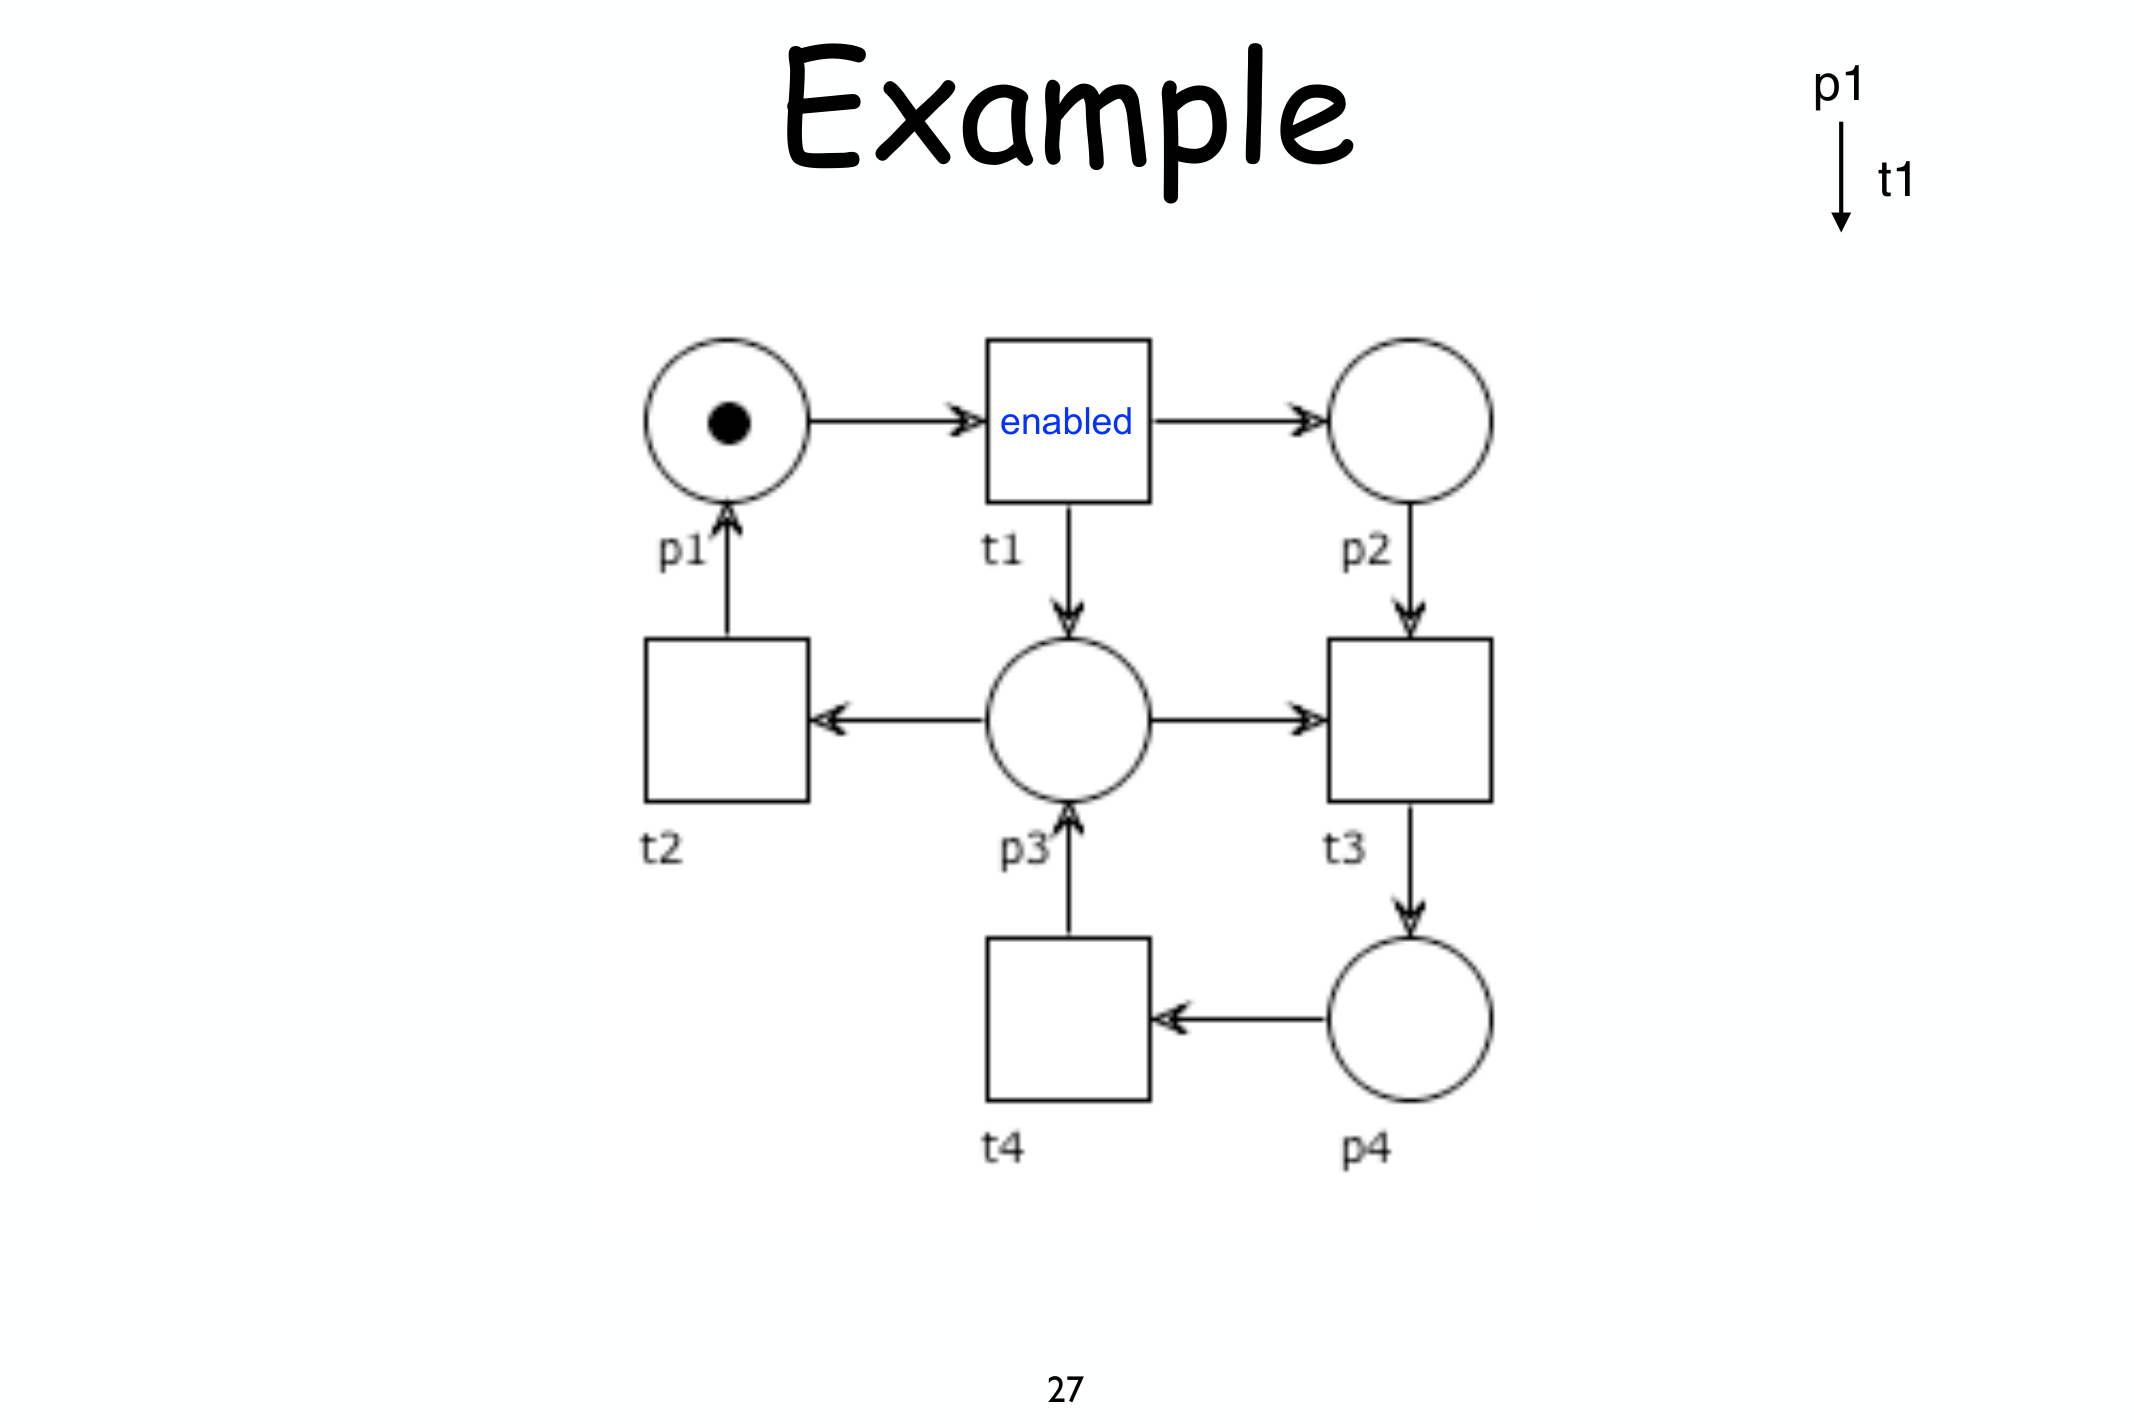
\includegraphics[width=0.74\linewidth,height=0.34\textheight,keepaspectratio]{images/22-esercizi_p27_token-game-net.png}
\caption{Stato iniziale $M_0 = p_1$: solo $t_1$ è enabled (il suo unico input $p_1$ ha il token).}
\end{figure}

Seguiamo lo scatto passo-passo:

\begin{boxexample}{La sequenza di scatti}
\textbf{Passo 1} — enabled: $t_1$ (unico input $p_1$ marcato).

\[
M_0 = p_1 \ \xrightarrow{\ t_1\ }\ M_1 = p_2+p_3
\]

\textbf{Passo 2} — enabled: $t_2$ (via $p_3$) e $t_3$ (via $p_2,p_3$). Scatta $t_2$.

\[
M_1 = p_2+p_3 \ \xrightarrow{\ t_2\ }\ M_2 = p_1+p_2
\]

\textbf{Passo 3} — enabled: $t_1$. $p_2$ aveva già un token, ora ne ha due.

\[
M_2 = p_1+p_2 \ \xrightarrow{\ t_1\ }\ M_3 = 2p_2+p_3
\]

\textbf{Passo 4} — enabled: $t_3$ (consuma un token da $p_2$ e uno da $p_3$).

\[
M_3 = 2p_2+p_3 \ \xrightarrow{\ t_3\ }\ M_4 = p_2+p_4
\]

\textbf{Passo 5} — enabled: $t_4$.

\[
M_4 = p_2+p_4 \ \xrightarrow{\ t_4\ }\ M_5 = p_2+p_3
\]

Da qui il gioco continua: $M_5$ è già lo stato visto al passo 2, il ciclo si ripete.
\end{boxexample}

\begin{figure}[!htb]
\centering
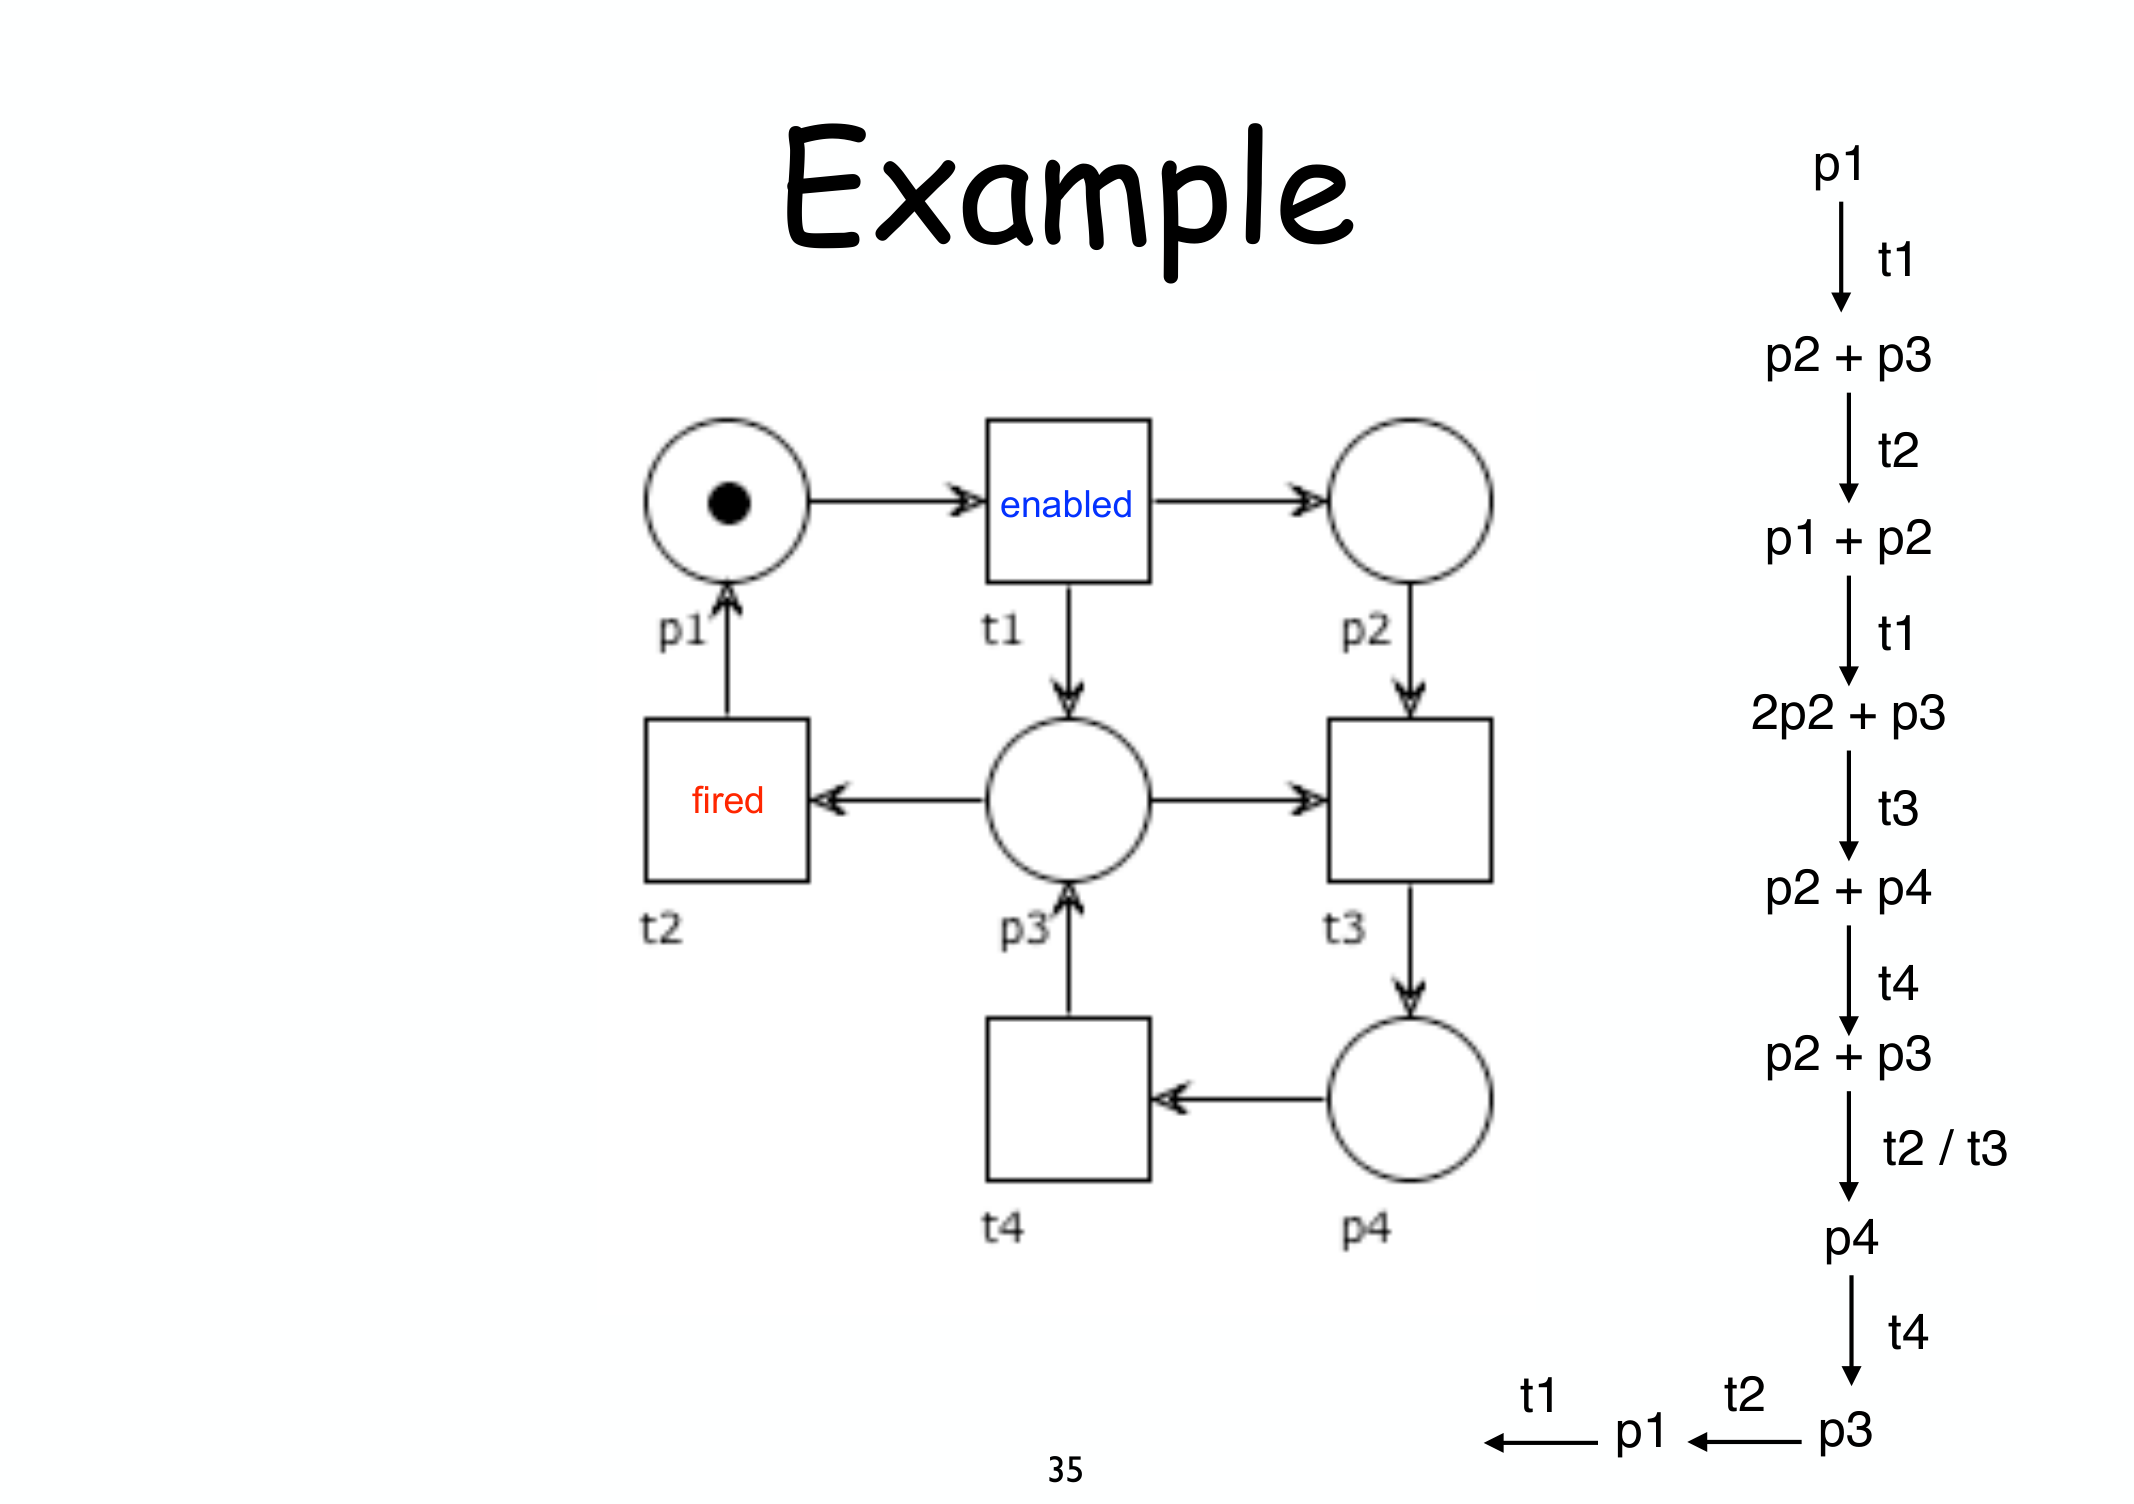
\includegraphics[width=0.74\linewidth,height=0.34\textheight,keepaspectratio]{images/22-esercizi_p35_token-game-trace.png}
\caption{L'intera traccia in un colpo d'occhio: ogni riga è "marcatura $\rightarrow$ scatto $\rightarrow$ marcatura successiva". Nota come al passo \texttt{t2/t3} la marcatura $p_2+p_3$ riabiliti \textbf{entrambe} le transizioni: nel disegno si segue il ramo di $t_3$, ma $t_2$ era ugualmente possibile.}
\end{figure}

\begin{boxwarning}{Occhio alla molteplicità}
Al passo 3:

\[
M_2 = p_1+p_2 \ \xrightarrow{\ t_1\ }\ M_3
\]

$t_1$ produce \textbf{un} token in $p_2$ e \textbf{uno} in $p_3$, che si sommano a quelli già presenti — $p_2$ passa da 1 a 2 token. Il token game \textbf{non sostituisce} i contenuti dei place, li \textbf{somma/sottrae}.
\end{boxwarning}

\section{\texorpdfstring{2. Costruire il reachability graph (algoritmo BFS)}{2. Costruire il reachability graph (algoritmo BFS)}}

\emph{Teoria: \hyperref[ch:09]{09 — Occurrence Graph}.}

L'algoritmo è una visita in ampiezza (BFS) sull'insieme delle marcature raggiungibili:

\begin{boxnote}{Algoritmo}
\begin{enumerate}
\item \texttt{Todo = \{M0\}}, \texttt{Nodes = \{\}}, \texttt{Arcs = \{\}}.
\item Estrai una marcatura $M$ da \texttt{Todo}, aggiungila a \texttt{Nodes}.
\item Per \textbf{ogni} transition enabled in $M$, calcola la marcatura successiva $M'$ e registra l'arco $(M,t,M')$.
\item Le $M'$ \textbf{mai viste prima} (né in \texttt{Nodes} né in \texttt{Todo}) vanno aggiunte a \texttt{Todo}.
\item Ripeti finché \texttt{Todo} non è vuoto.
\end{enumerate}
\end{boxnote}

Applichiamolo a un semaforo singolo: 3 place (\texttt{red}, \texttt{green}, \texttt{yellow}), 3 transition (\texttt{go-green}, \texttt{go-yellow}, \texttt{go-red}), $M_0=\text{red}$.

\begin{figure}[!htb]
\centering
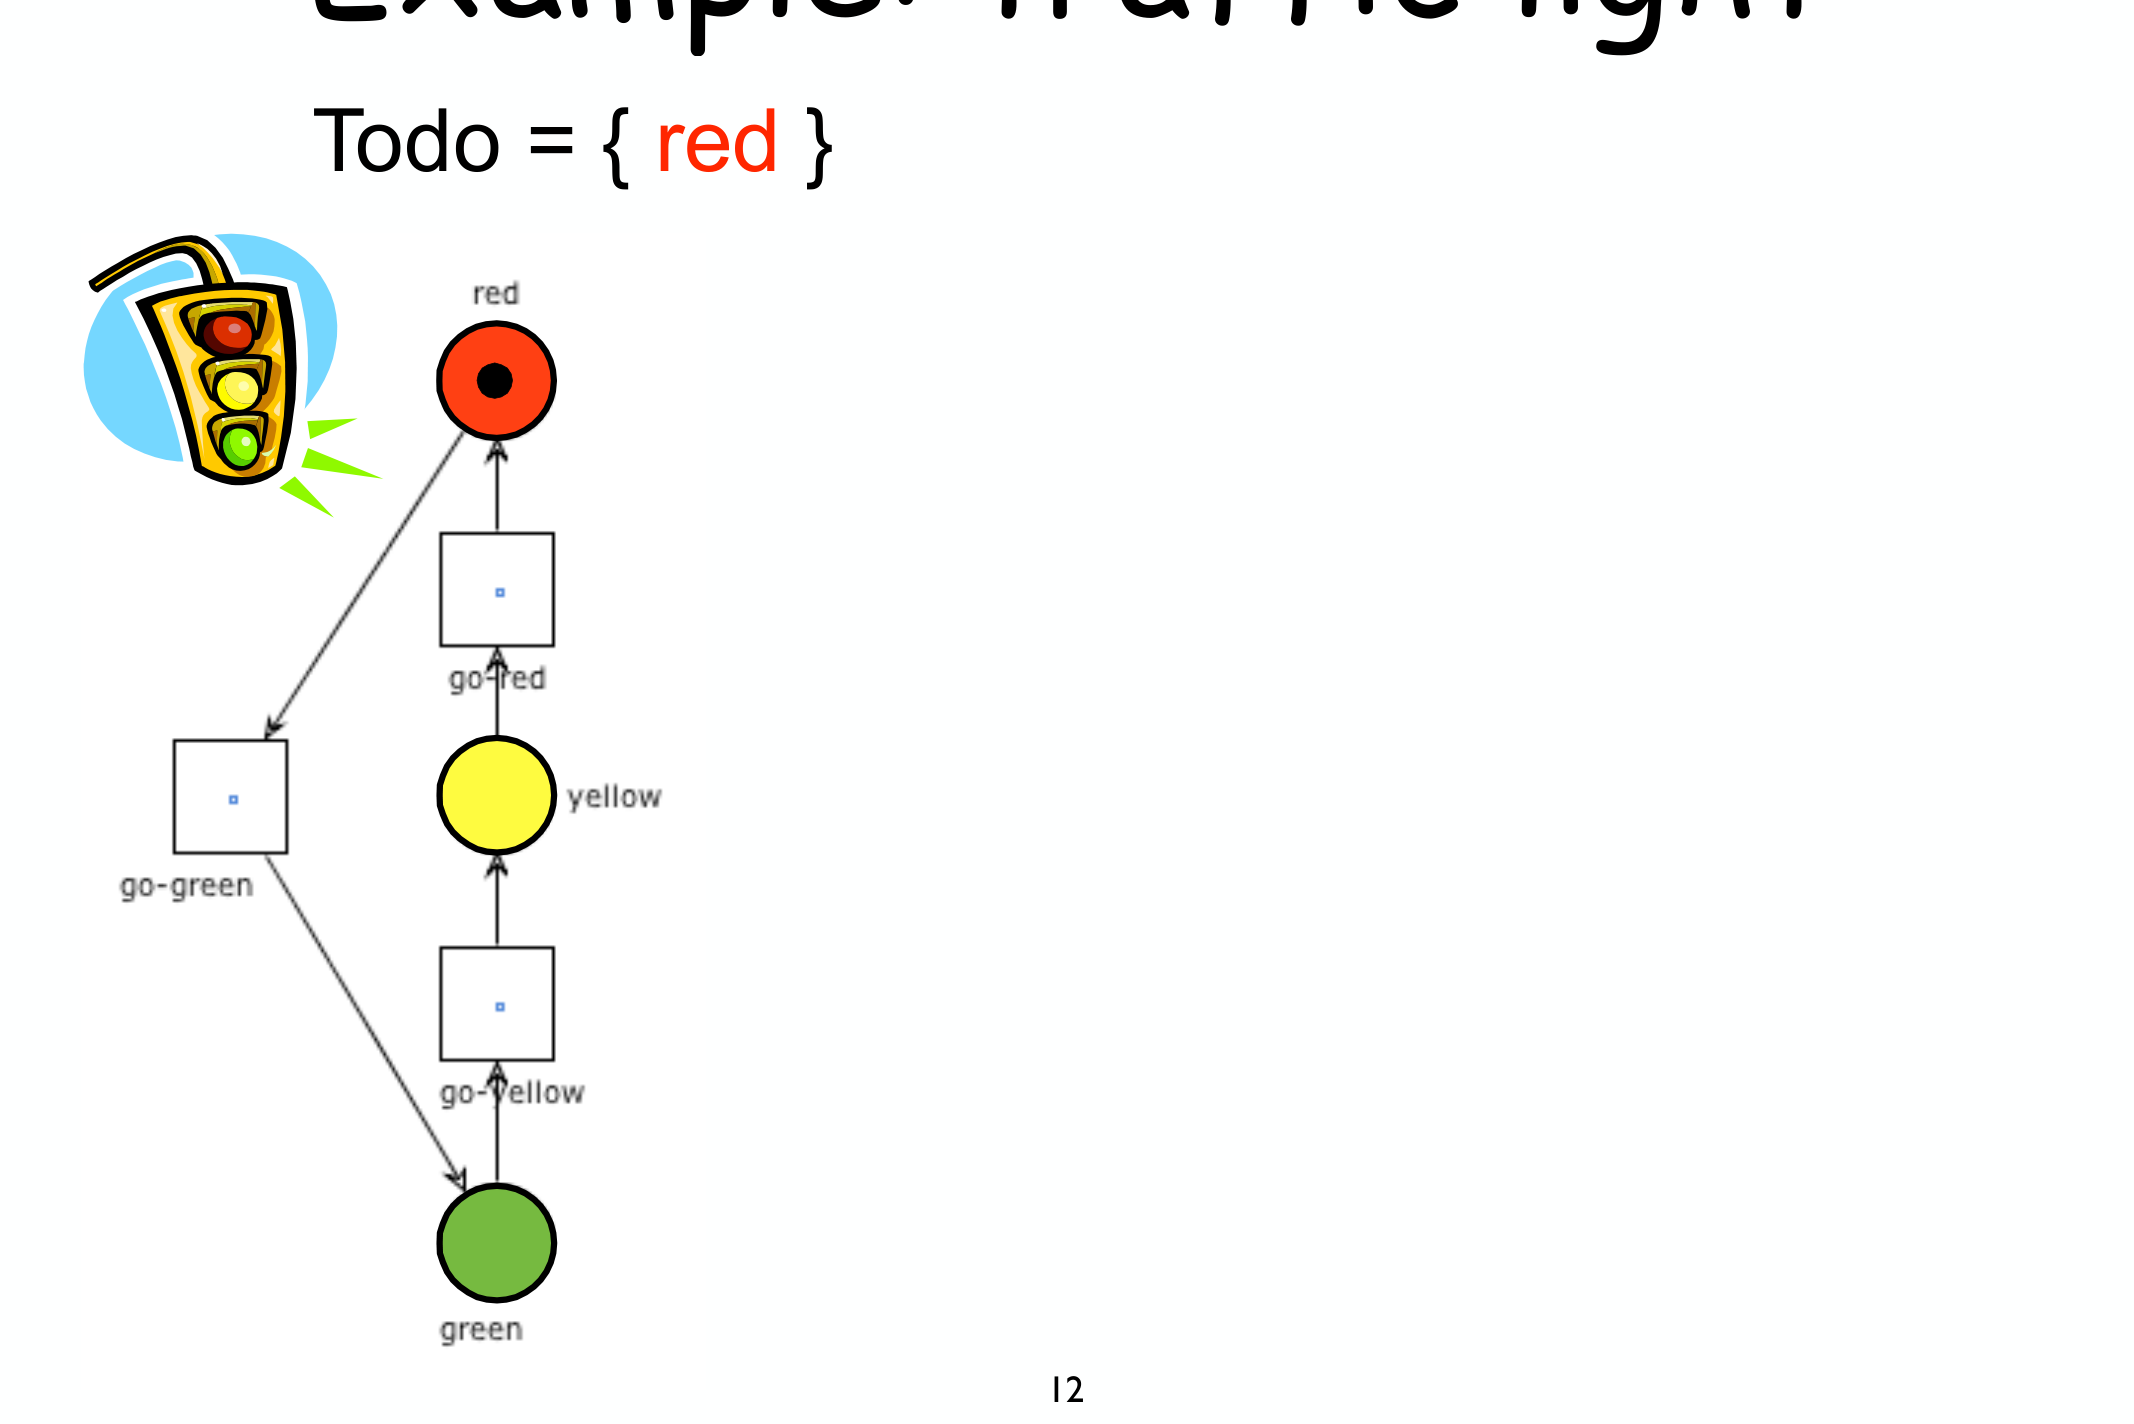
\includegraphics[width=0.74\linewidth,height=0.34\textheight,keepaspectratio]{images/22-esercizi_p12_rg-step1.png}
\caption{Passo 1: si esplora \texttt{red}, l'unica marcatura in \texttt{Todo}. È enabled solo \texttt{go-green} (il suo unico input è \texttt{red}), che porta a \texttt{green} — nuova, va aggiunta a \texttt{Todo}.}
\end{figure}

\begin{boxexample}{Il resto della BFS}
\begin{itemize}
\item \texttt{Todo=\{green\}}: esploro \texttt{green} $\rightarrow$ enabled \texttt{go-yellow} $\rightarrow$ produce \texttt{yellow} (nuova) $\rightarrow$ \texttt{Todo=\{yellow\}}.
\item \texttt{Todo=\{yellow\}}: esploro \texttt{yellow} $\rightarrow$ enabled \texttt{go-red} $\rightarrow$ produce \texttt{red} (\textbf{già in Nodes}, non si riaggiunge) $\rightarrow$ \texttt{Todo=\{\}}.
\item \texttt{Todo} vuoto: \textbf{fine}. Il reachability graph ha 3 nodi e 3 archi, ed è esso stesso un ciclo.
\end{itemize}
\end{boxexample}

\begin{figure}[!htb]
\centering
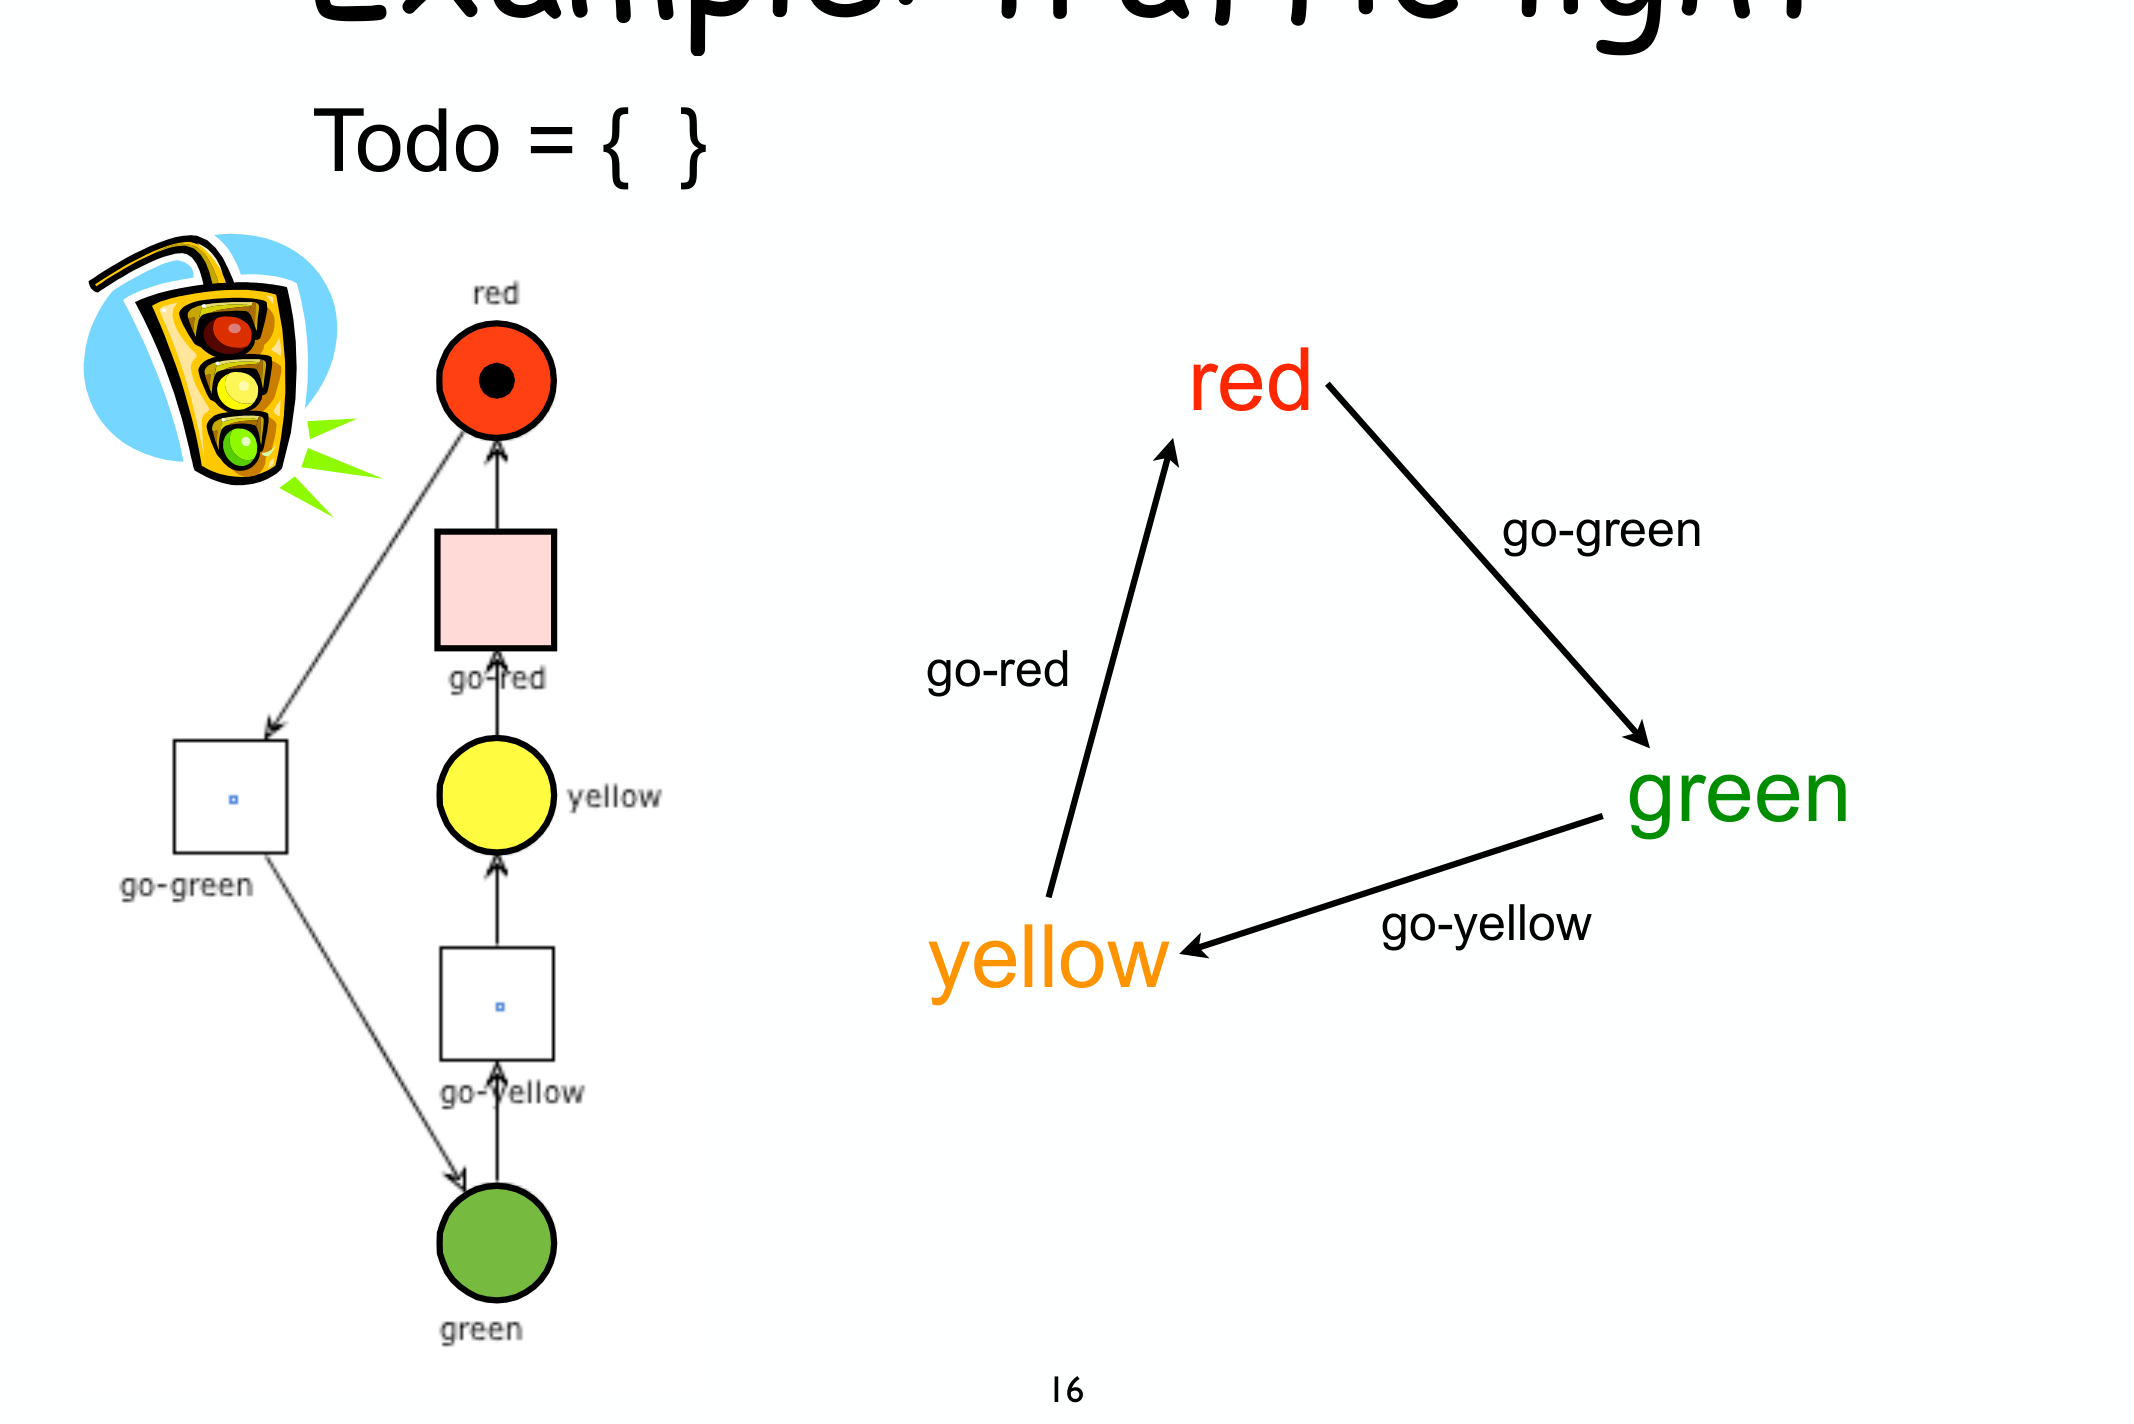
\includegraphics[width=0.74\linewidth,height=0.34\textheight,keepaspectratio]{images/22-esercizi_p16_rg-final.png}
\caption{Il reachability graph completo: un triangolo orientato. Da qualunque stato si può tornare a \texttt{red} — la rete è ciclica, e (essendo un solo token che gira) anche live e safe.}
\end{figure}

\begin{boxtip}{La regola pratica}
Ogni volta che generi una nuova marcatura, \textbf{controllala contro tutte quelle già viste} (in \texttt{Nodes} \emph{e} in \texttt{Todo}) prima di aggiungerla: è l'unico modo per evitare di esplorare la stessa marcatura due volte (e per accorgersi che il grafo è finito, se lo è).
\end{boxtip}

\section{\texorpdfstring{3. Matrice di incidenza e marking equation}{3. Matrice di incidenza e marking equation}}

\emph{Teoria: \hyperref[ch:11]{11 — Net Matrices}.}

Costruiamo la \textbf{incidence matrix} $\mathbf{N}$ di una rete (righe = place, colonne = transition):

\[
\mathbf{N}(p,t) =
\begin{cases}
-1 & \text{se } p\in\bullet t\setminus t\bullet \\[4pt]
+1 & \text{se } p\in t\bullet\setminus\bullet t \\[4pt]
\phantom{+}0 & \text{altrimenti}
\end{cases}
\]

sul distributore automatico con 5 place e 5 transition.

\begin{figure}[!htb]
\centering
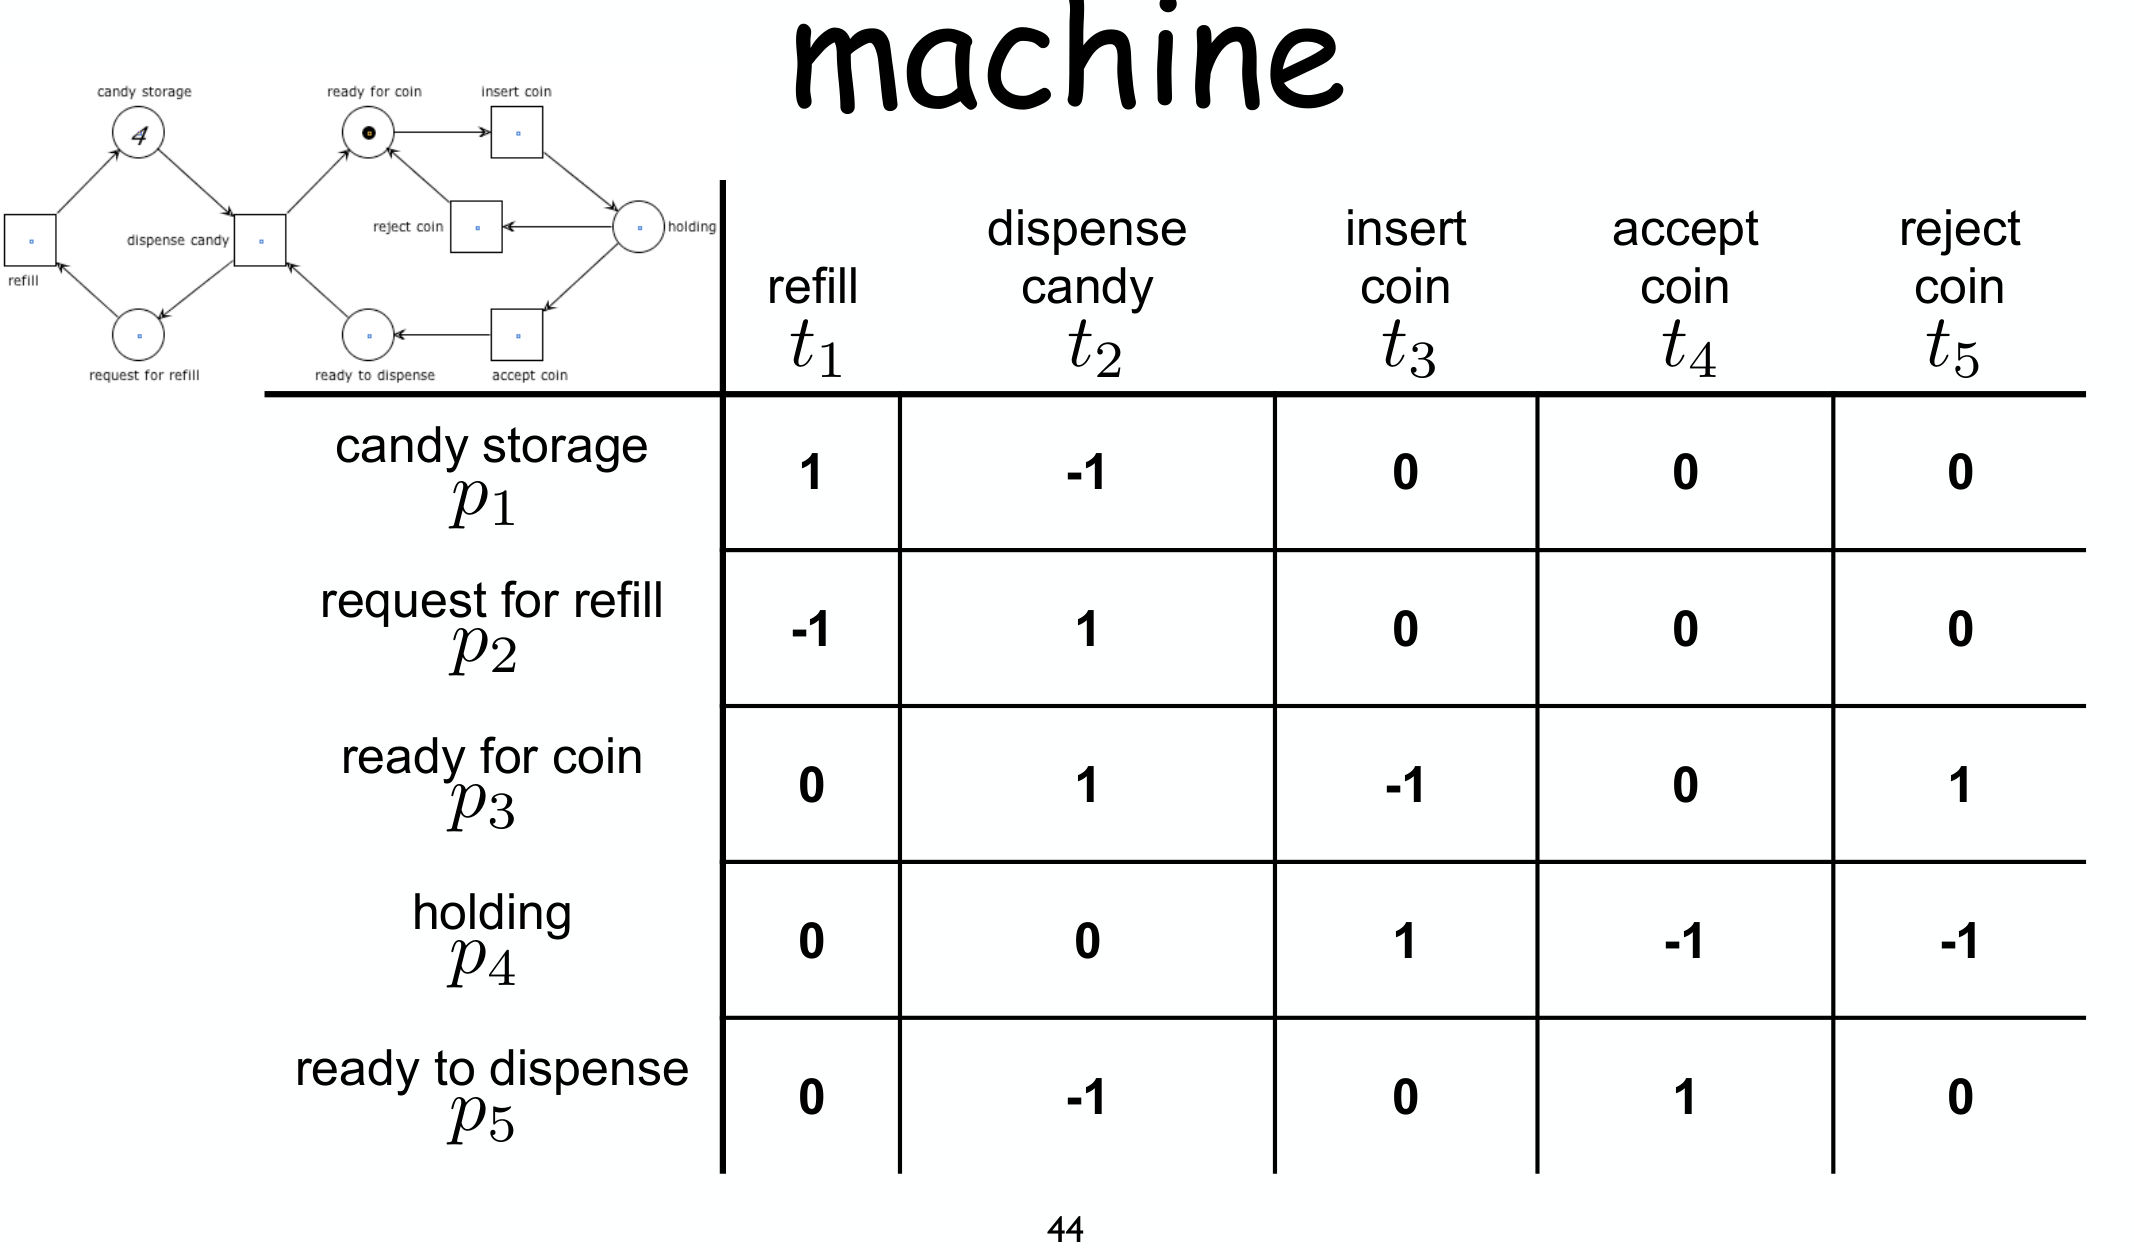
\includegraphics[width=0.74\linewidth,height=0.34\textheight,keepaspectratio]{images/11-net-matrices_p42_vending-incidence.png}
\caption{La matrice si legge colonna per colonna: la colonna di \texttt{dispense candy} ($t_2$) ha $-1$ su \texttt{candy storage} (consuma candy) e $+1$ su \texttt{request for refill} e $-1$ su \texttt{ready to dispense}... ogni colonna è il "bilancio" di quella transition su ogni place.}
\end{figure}

La \textbf{marking equation} dice che, dopo una firing sequence $\sigma$ con Parikh vector $\vec\sigma$ (quante volte compare ogni transition), la marcatura finale si calcola \textbf{senza simulare passo-passo}:

\[
M' = M_0 + \mathbf{N}\cdot\vec\sigma
\]

\begin{boxexample}{Applicarla}
Marcatura iniziale e sequenza da riprodurre:

\[
M_0 = [4,0,1,0,0] \qquad\qquad \sigma = t_3\,t_5\,t_3\,t_4\,t_2
\]

Il Parikh vector conta quante volte compare ciascuna transition ($t_1$ zero volte, $t_2$ una volta, $t_3$ due volte, $t_4$ una volta, $t_5$ una volta):

\[
\vec\sigma = [0,1,2,1,1]
\]

Si calcola $M_0 + \mathbf{N}\cdot\vec\sigma$ moltiplicando la matrice per il vettore colonna e sommando a $M_0$.
\end{boxexample}

\begin{figure}[!htb]
\centering
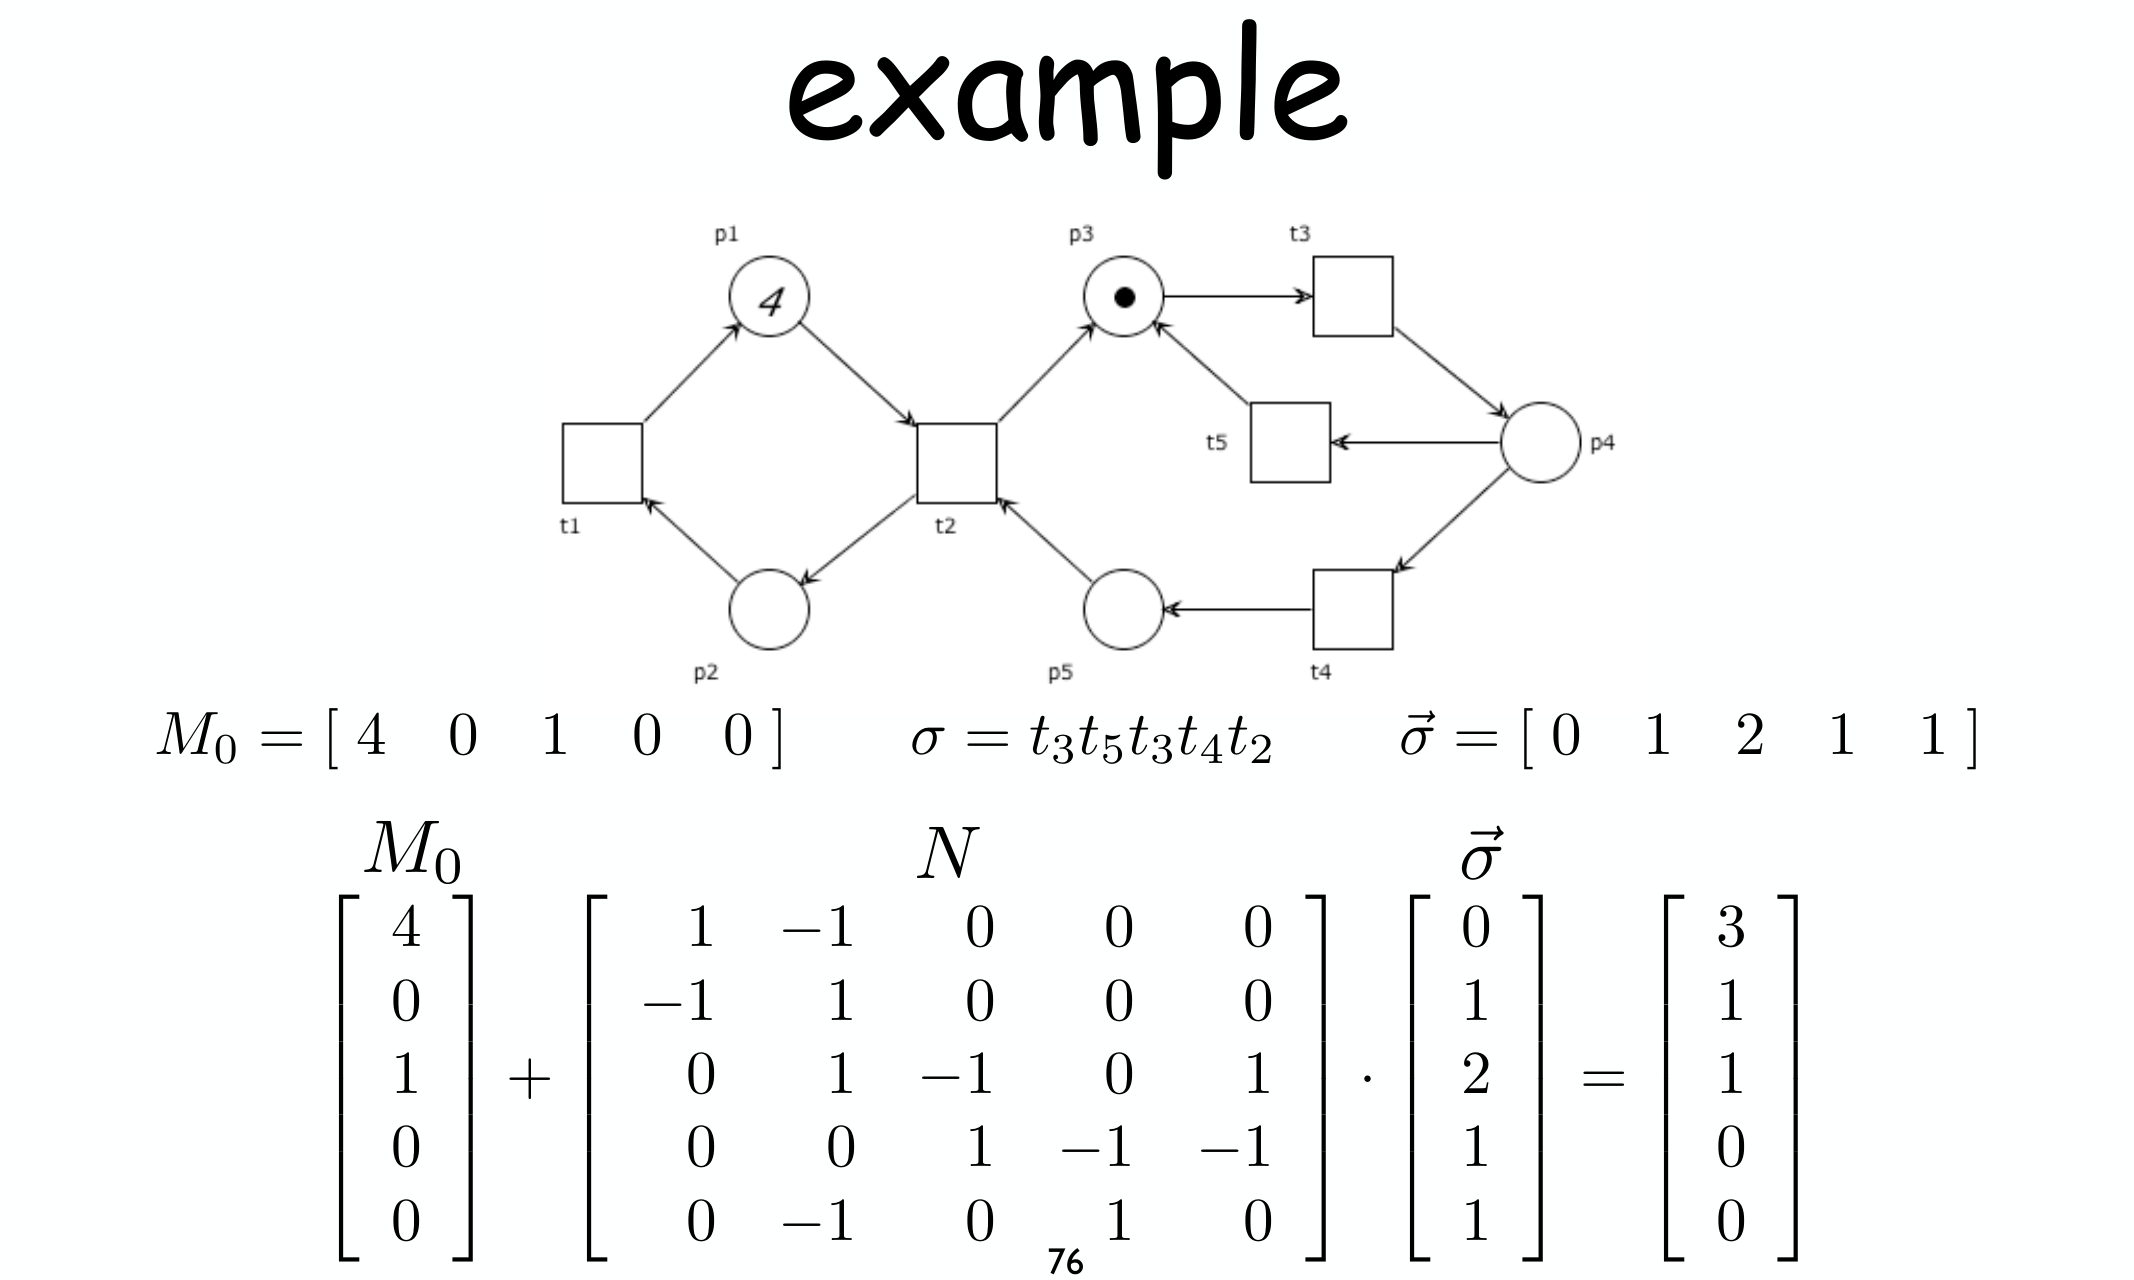
\includegraphics[width=0.74\linewidth,height=0.34\textheight,keepaspectratio]{images/11-net-matrices_p74_marking-equation.png}
\caption{Il conto fatto fino in fondo.}
\end{figure}

\[
M_0 + \mathbf{N}\vec\sigma = [3,1,1,0,0]
\]

\begin{boxwarning}{Nota bene}
Questo calcolo \textbf{non dice se $\sigma$ è davvero eseguibile} (per quello serve verificare passo passo che ogni transition trovi i token) — dice solo \emph{dove si arriverebbe se lo fosse}. È lo strumento perfetto per il \textbf{test negativo}: se il risultato non torna con una marcatura attesa, quella marcatura \textbf{di sicuro non è raggiungibile} con quel $\vec\sigma$.
\end{boxwarning}

\section{\texorpdfstring{4. Calcolare S-invariant e T-invariant risolvendo un sistema lineare}{4. Calcolare S-invariant e T-invariant risolvendo un sistema lineare}}

\emph{Teoria: \hyperref[ch:14]{14 — Invariants}.}

Riprendiamo la rete della sezione 1 e cerchiamone gli invarianti \textbf{a mano}:

\[
\begin{aligned}
t_1&: p_1\to p_2,p_3 \\[4pt]
t_2&: p_3\to p_1 \\[4pt]
t_3&: p_2,p_3\to p_4 \\[4pt]
t_4&: p_4\to p_3
\end{aligned}
\]

\begin{figure}[!htb]
\centering
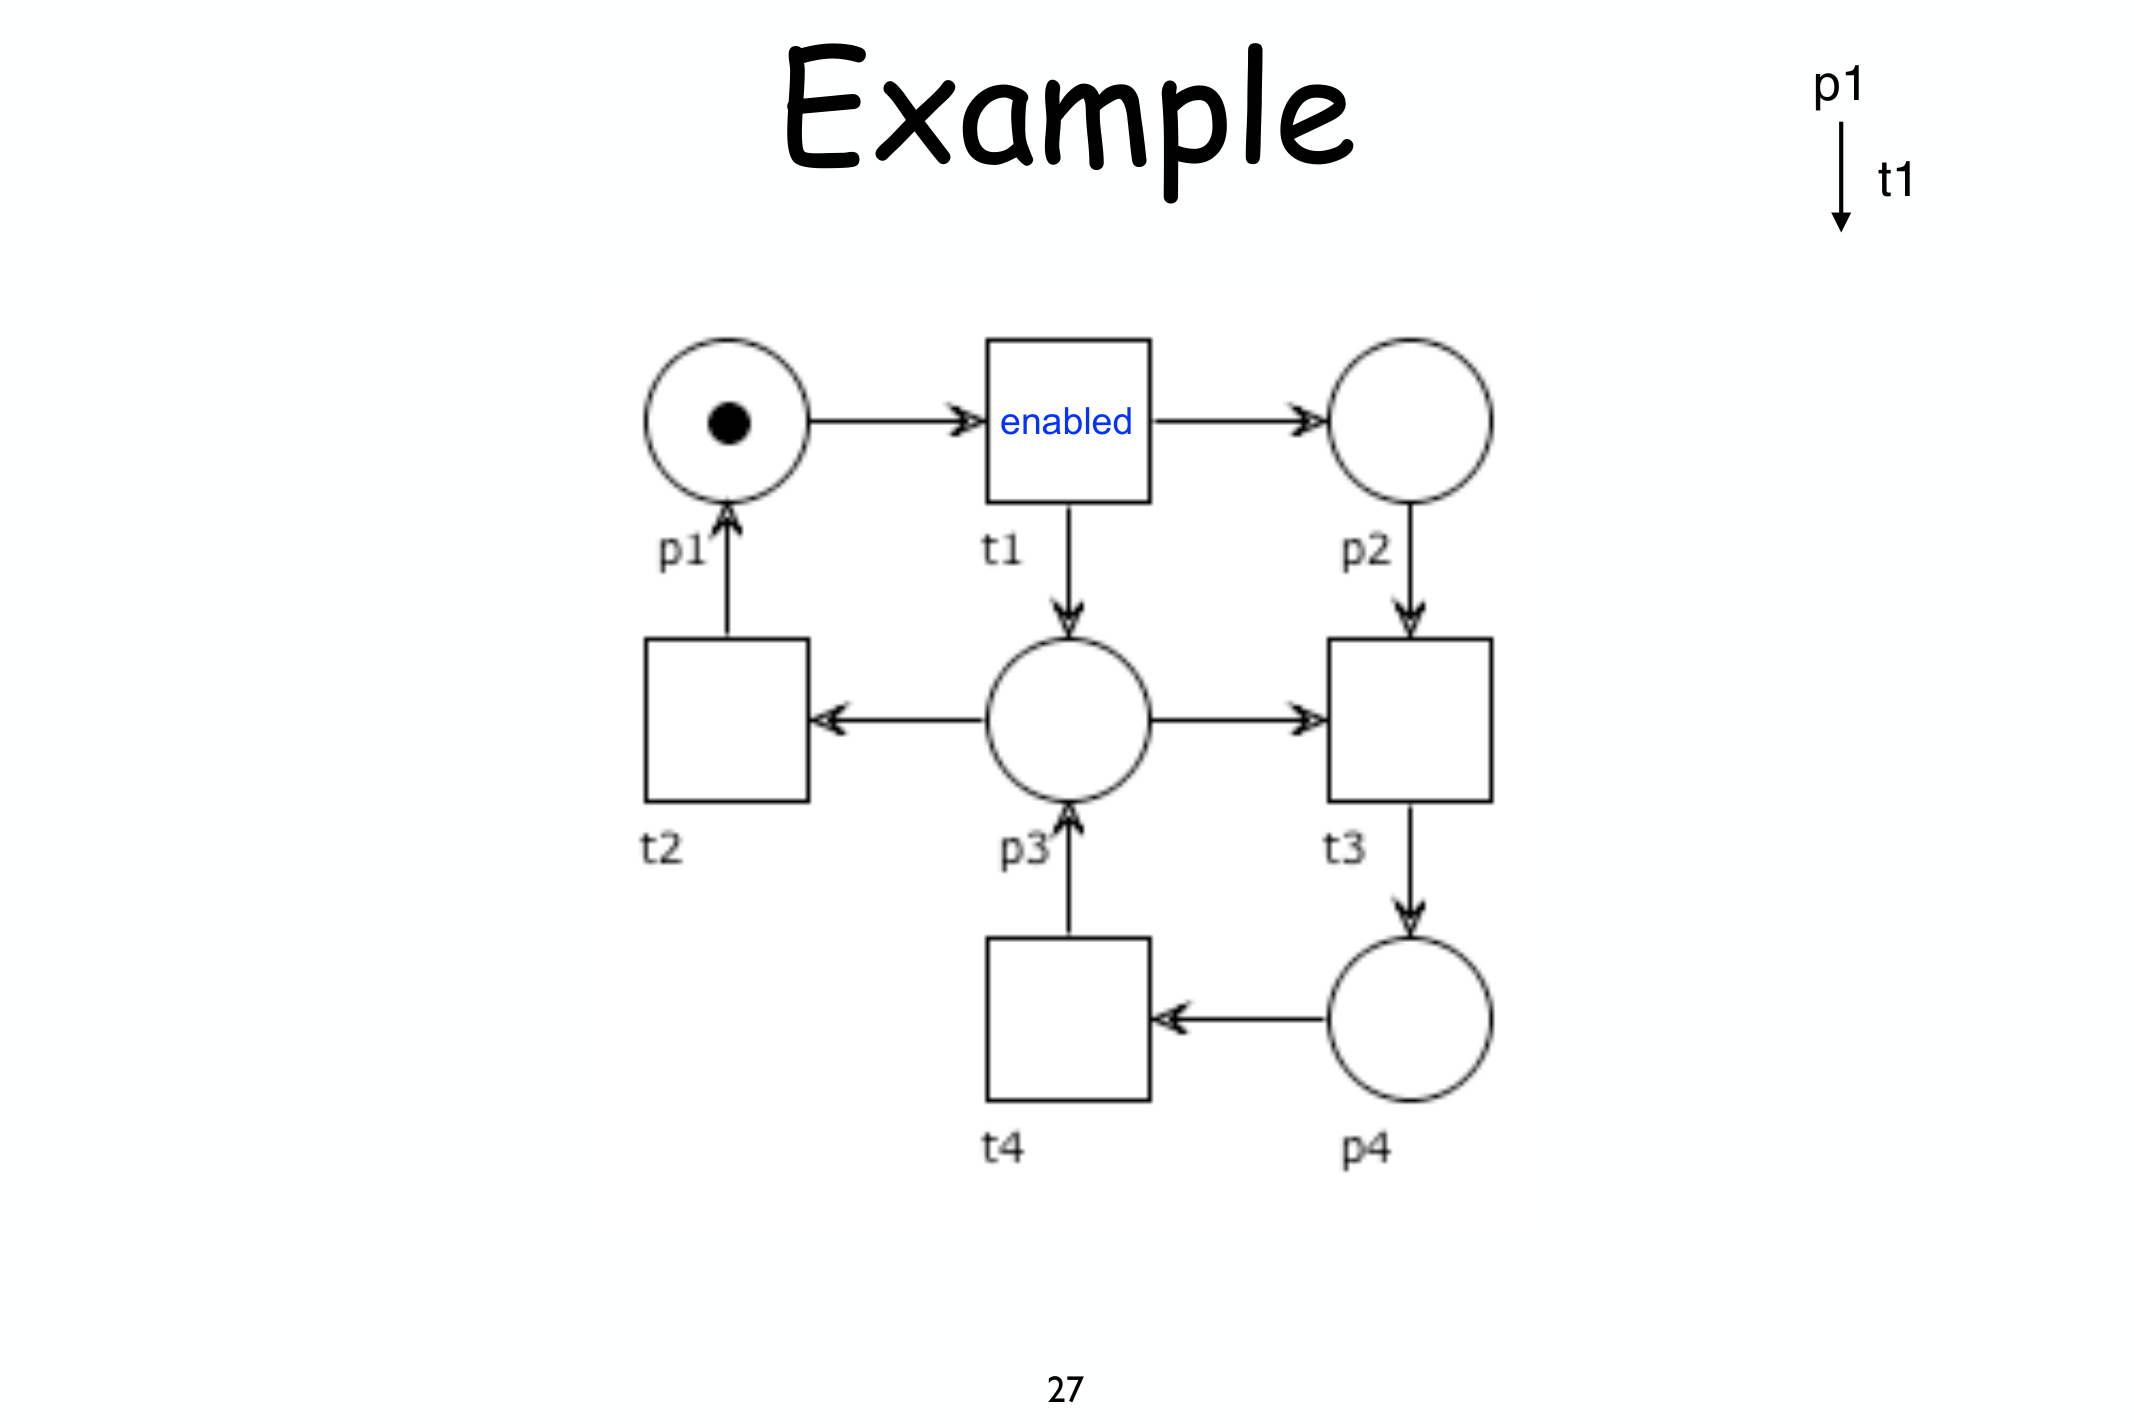
\includegraphics[width=0.74\linewidth,height=0.34\textheight,keepaspectratio]{images/22-esercizi_p27_token-game-net.png}
\caption{La rete da analizzare algebricamente.}
\end{figure}

\textbf{Passo 1 — matrice di incidenza} (righe $p_1..p_4$, colonne $t_1..t_4$):

\begingroup\small
\begin{tabularx}{\linewidth}{>{\raggedright\arraybackslash}X>{\raggedright\arraybackslash}X>{\raggedright\arraybackslash}X>{\raggedright\arraybackslash}X>{\raggedright\arraybackslash}X}
\toprule
\textbf{} & \textbf{$t_1$} & \textbf{$t_2$} & \textbf{$t_3$} & \textbf{$t_4$} \\
\midrule
$p_1$ & $-1$ & $+1$ & $0$ & $0$ \\
$p_2$ & $+1$ & $0$ & $-1$ & $0$ \\
$p_3$ & $+1$ & $-1$ & $-1$ & $+1$ \\
$p_4$ & $0$ & $0$ & $+1$ & $-1$ \\
\bottomrule
\end{tabularx}
\endgroup

\subsection{\texorpdfstring{S-invariant: risolvere $I\cdot\mathbf{N}=\mathbf{0}$}{S-invariant: risolvere IN=0}}

\textbf{Passo 2} — imponi, per ogni \textbf{colonna} (transition), "peso consumato = peso prodotto": con $I=[I_1,I_2,I_3,I_4]$,

\[
\begin{cases}
t_1:\ -I_1+I_2+I_3=0\\
t_2:\ I_1-I_3=0\\
t_3:\ -I_2-I_3+I_4=0\\
t_4:\ I_3-I_4=0
\end{cases}
\]

\textbf{Passo 3} — risolvi: da $t_2$, $I_1=I_3$; da $t_4$, $I_3=I_4$; sostituendo in $t_1$:

\[
-I_3+I_2+I_3=0 \ \Longrightarrow\ I_2=0
\]

(e $t_3$ è automaticamente soddisfatta). Soluzione generale:

\[
I = [k,\ 0,\ k,\ k]
\]

\begin{boxexample}{Risultato}
Prendendo $k=1$:

\[
I = [1,\ 0,\ 1,\ 1]
\]

è un S-invariant. È \textbf{semi-positive} ($I\ge 0$, non tutto zero) ma \textbf{non positive} (il peso su $p_2$ è $0$).
\end{boxexample}

\begin{boxwarning}{Il punto sottile: cosa NON certifica un invariante semi-positive}
Da \hyperref[ch:14]{14 — Invariants}: solo un S-invariant \textbf{positive} certifica la boundedness di \textbf{tutti} i place. Qui $p_2$ ha peso $0$, quindi $I$ \textbf{non dice nulla} su $p_2$. E infatti $p_2$ è \textbf{davvero unbounded}: basta scattare ripetutamente $t_1,t_2,t_1,t_2,\dots$ (mai $t_3$) per accumulare in $p_2$ un token in più a ogni giro, senza che nulla lo consumi. L'esempio mostra bene perché la teoria richiede \emph{positive} e non solo \emph{semi-positive}.
\end{boxwarning}

\subsection{\texorpdfstring{T-invariant: risolvere $\mathbf{N}\cdot J=\mathbf{0}$}{T-invariant: risolvere N J=0}}

\textbf{Passo 2} — imponi, per ogni \textbf{riga} (place), "prodotto = consumato": con $J=[J_1,J_2,J_3,J_4]$,

\[
\begin{cases}
p_1:\ -J_1+J_2=0\\
p_2:\ J_1-J_3=0\\
p_3:\ J_1-J_2-J_3+J_4=0\\
p_4:\ J_3-J_4=0
\end{cases}
\]

\textbf{Passo 3} — risolvi: $J_1=J_2$ (da $p_1$), $J_1=J_3$ (da $p_2$), $J_3=J_4$ (da $p_4$); sostituendo in $p_3$:

\[
J_1-J_1-J_1+J_1=0 \qquad\checkmark\ \text{sempre vera}
\]

Soluzione:

\[
J = [k,\ k,\ k,\ k]
\]

\begin{boxexample}{Risultato}
Con $k=1$:

\[
J = [1,\ 1,\ 1,\ 1] \qquad \textbf{positive}
\]

Significa: esiste una sequenza che usa \textbf{ogni transition esattamente una volta} e riporta la rete alla marcatura di partenza (nell'esempio: $t_1,t_3,t_4,t_2$ in un ordine compatibile fa proprio questo).
\end{boxexample}

\section{\texorpdfstring{5. Verificare la soundness: costruire $N^\star$ e leggere il reachability graph a tre colori}{5. Verificare la soundness: costruire N\textasciicircum{} e leggere il reachability graph a tre colori}}

\emph{Teoria: \hyperref[ch:12]{12 — Soundness}, \hyperref[ch:21]{21 — WFnets Diagnosis}.}

Prendiamo il workflow net "register $\rightarrow$ send/dont $\rightarrow$ rec/timeout $\rightarrow$ process/redo/done $\rightarrow$ archive" già visto in \hyperref[ch:21]{21 — WFnets Diagnosis} (place $i, c_1, c_2, c_3, c_4, c_5, c_6, c_7, c_8, o$).

\begin{boxnote}{Passo 1 — costruire $N^\star$}
Aggiungi la transition \textbf{reset}:

\[
\bullet\,\text{reset} = \{o\} \qquad\qquad \text{reset}\,\bullet = \{i\}
\]

Ora la rete è ciclica e puoi costruire il reachability graph \textbf{finito} (assumendo che sia bounded — altrimenti serve il coverability graph, vedi \hyperref[ch:21]{21 — WFnets Diagnosis}).
\end{boxnote}

\begin{boxnote}{Passo 2 — colorare gli stati del RG}
\begin{itemize}
\item \textbf{verde}: da qui \emph{ogni} cammino arriva a $o$;
\item \textbf{rosso}: da qui \emph{nessun} cammino arriva a $o$;
\item \textbf{giallo}: \emph{alcuni sì, altri no} — ancora recuperabile.
\end{itemize}
\end{boxnote}

\begin{figure}[!htb]
\centering
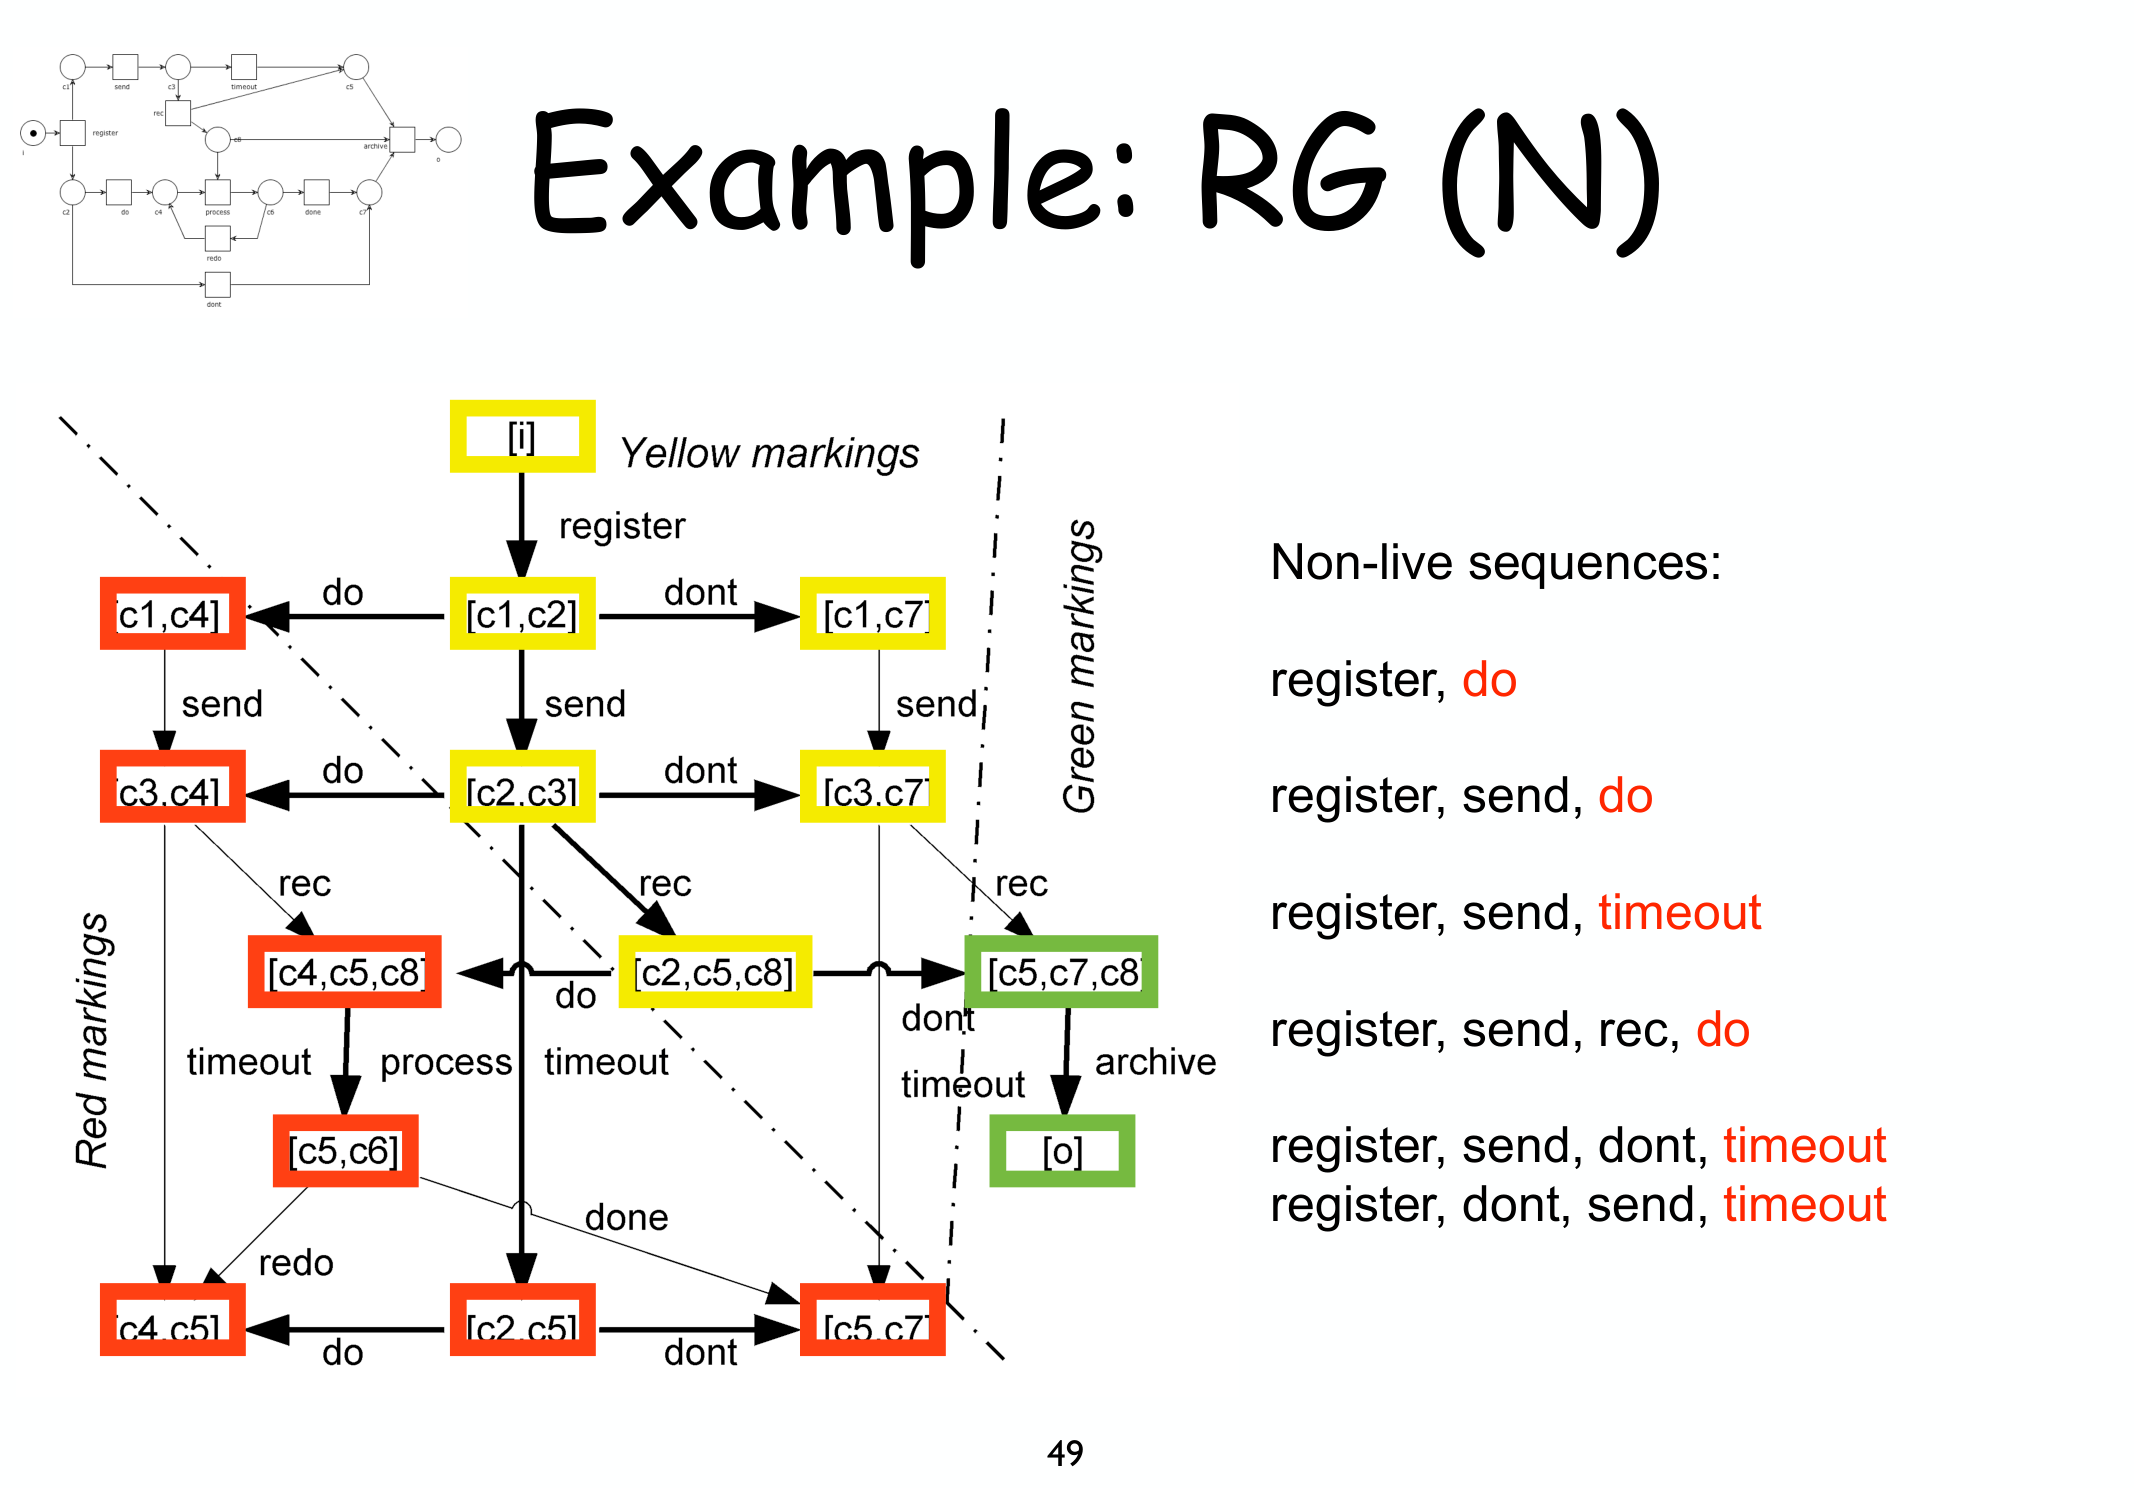
\includegraphics[width=0.74\linewidth,height=0.34\textheight,keepaspectratio]{images/21-wfnets-diagnosis_p49_rg-nonlive.png}
\caption{Applicato al nostro esempio: dallo stato iniziale (giallo) alcune scelte (es. \texttt{register} poi subito \texttt{do}) portano dritte al \textbf{rosso} — quella diramazione non potrà \textbf{mai più} completare il caso. Basta \textbf{una} non-live sequence per concludere che $N^\star$ \textbf{non è live}, quindi $N$ \textbf{non è sound}.}
\end{figure}

\begin{boxexample}{Come si legge in pratica}
\begin{enumerate}
\item Parti dallo stato iniziale $[i]$ (sempre giallo, a meno che la rete sia banale).
\item Segui gli scatti uno a uno; \textbf{appena} trovi uno stato da cui \emph{nessuno} dei successori porta al verde, coloralo \textbf{rosso}.
\item La sequenza di scatti che ti ha portato lì (es. \texttt{register, do}) è una \textbf{non-live sequence}: lo scenario più corto e concreto che mostra il difetto.
\item Se \textbf{non} trovi mai uno stato rosso (tutti gli stati sono verdi o gialli-che-diventano-verdi), allora $N^\star$ è live; controlla poi la boundedness per concludere sulla soundness.
\end{enumerate}
\end{boxexample}

\section{\texorpdfstring{6. Tradurre un EPC in Petri net, passo dopo passo}{6. Tradurre un EPC in Petri net, passo dopo passo}}

\emph{Teoria: \hyperref[ch:16a]{16a — EPC Analysis}.}

Prendiamo l'EPC "goods arrived $\rightarrow$ check goods $\rightarrow$ (ok / not ok $\rightarrow$ complaint $\rightarrow$ data revised) $\rightarrow$ store goods" con un ramo parallelo "record receipts of goods", e applichiamo i tre step.

\begin{figure}[!htb]
\centering
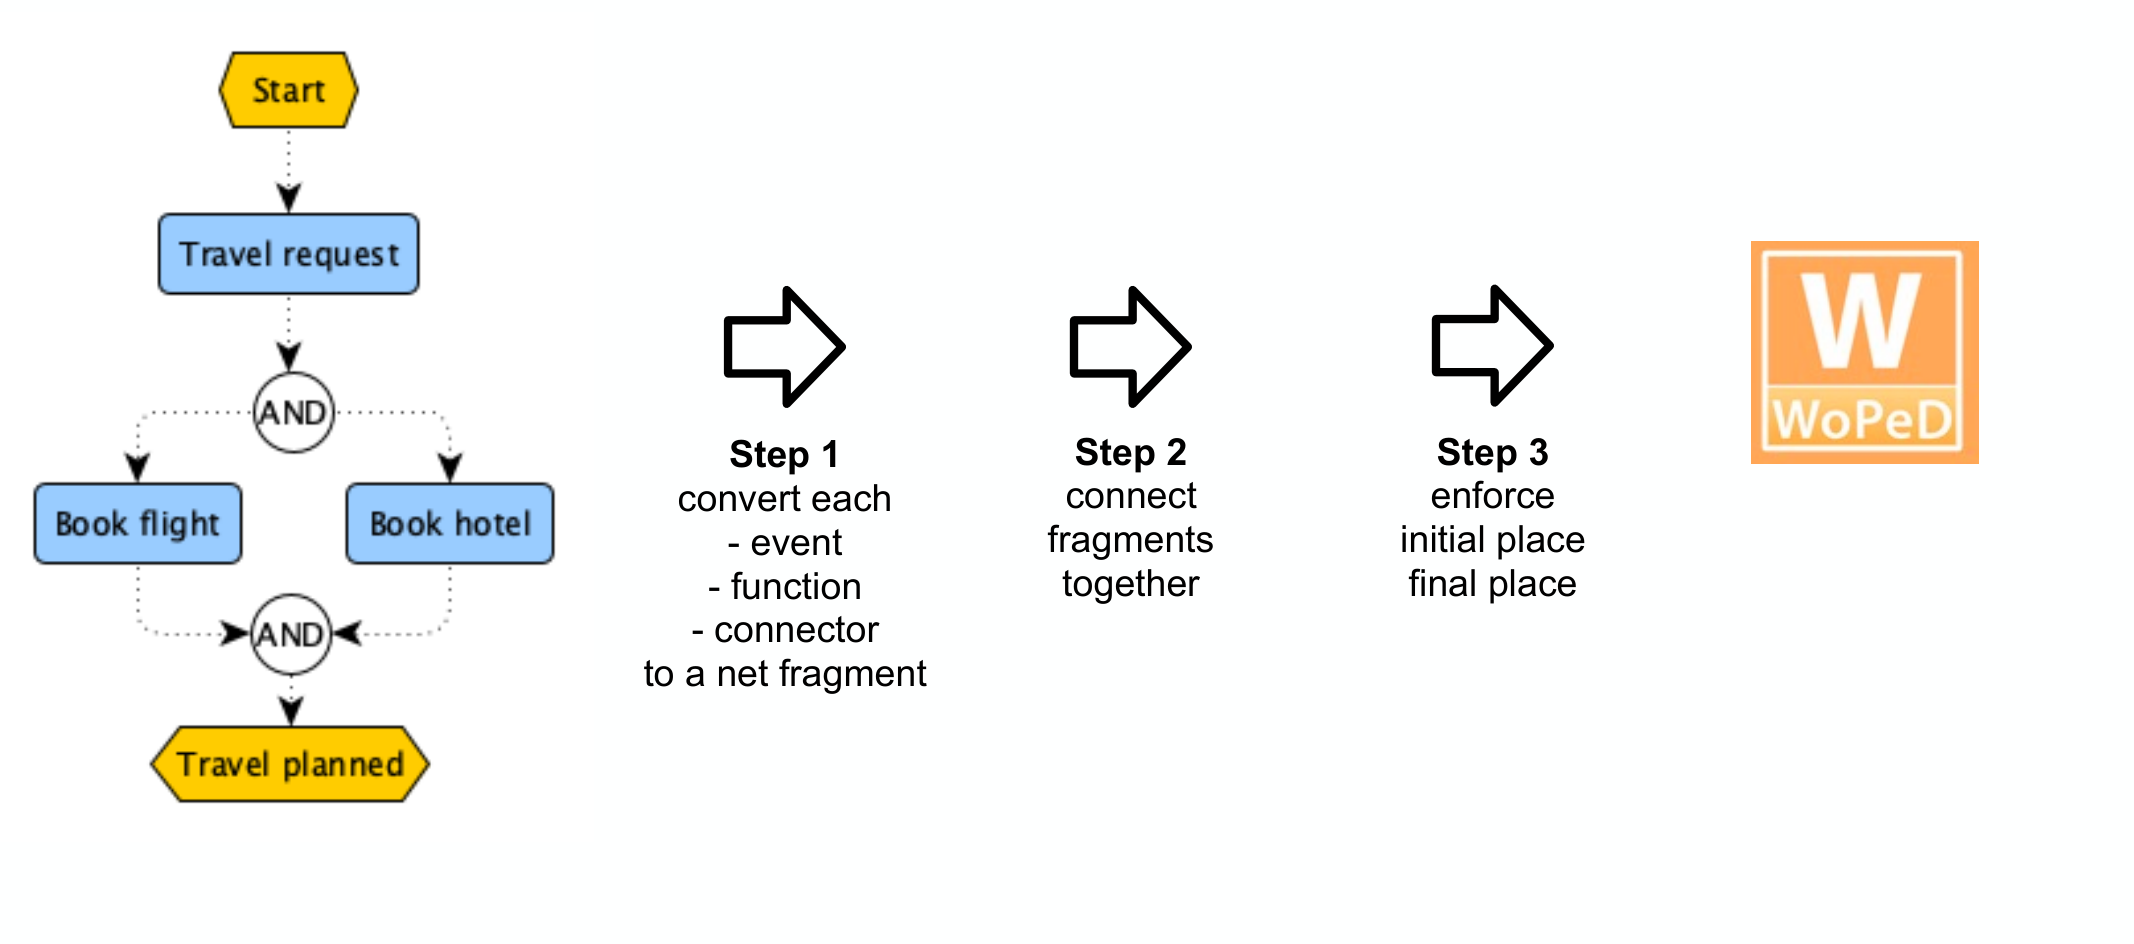
\includegraphics[width=0.74\linewidth,height=0.34\textheight,keepaspectratio]{images/16a-epc-analysis_p9_three-steps.png}
\caption{Il piano in tre mosse, da applicare in ordine.}
\end{figure}

\begin{boxexample}{Step 1 — frammenti locali}
\begin{itemize}
\item Ogni \textbf{event} $\rightarrow$ un place; ogni \textbf{function} $\rightarrow$ una transition (regola base, ricordando che per il \textbf{secondo/terzo approccio} la corrispondenza dipende dal contesto — vedi \hyperref[ch:16a]{16a — EPC Analysis}).
\item Il connettore \textbf{AND} dopo "check goods" (che porta sia a "ok/not ok" sia in parallelo a "record receipts") diventa una transition che produce \textbf{due} token, uno per ramo.
\item Il connettore \textbf{OR} finale (che riceve da "store goods" oppure da "record receipts", o da entrambi) si traduce come \textbf{xor + and} — la combinazione vista in dettaglio più sotto.
\end{itemize}
\end{boxexample}

\begin{figure}[!htb]
\centering
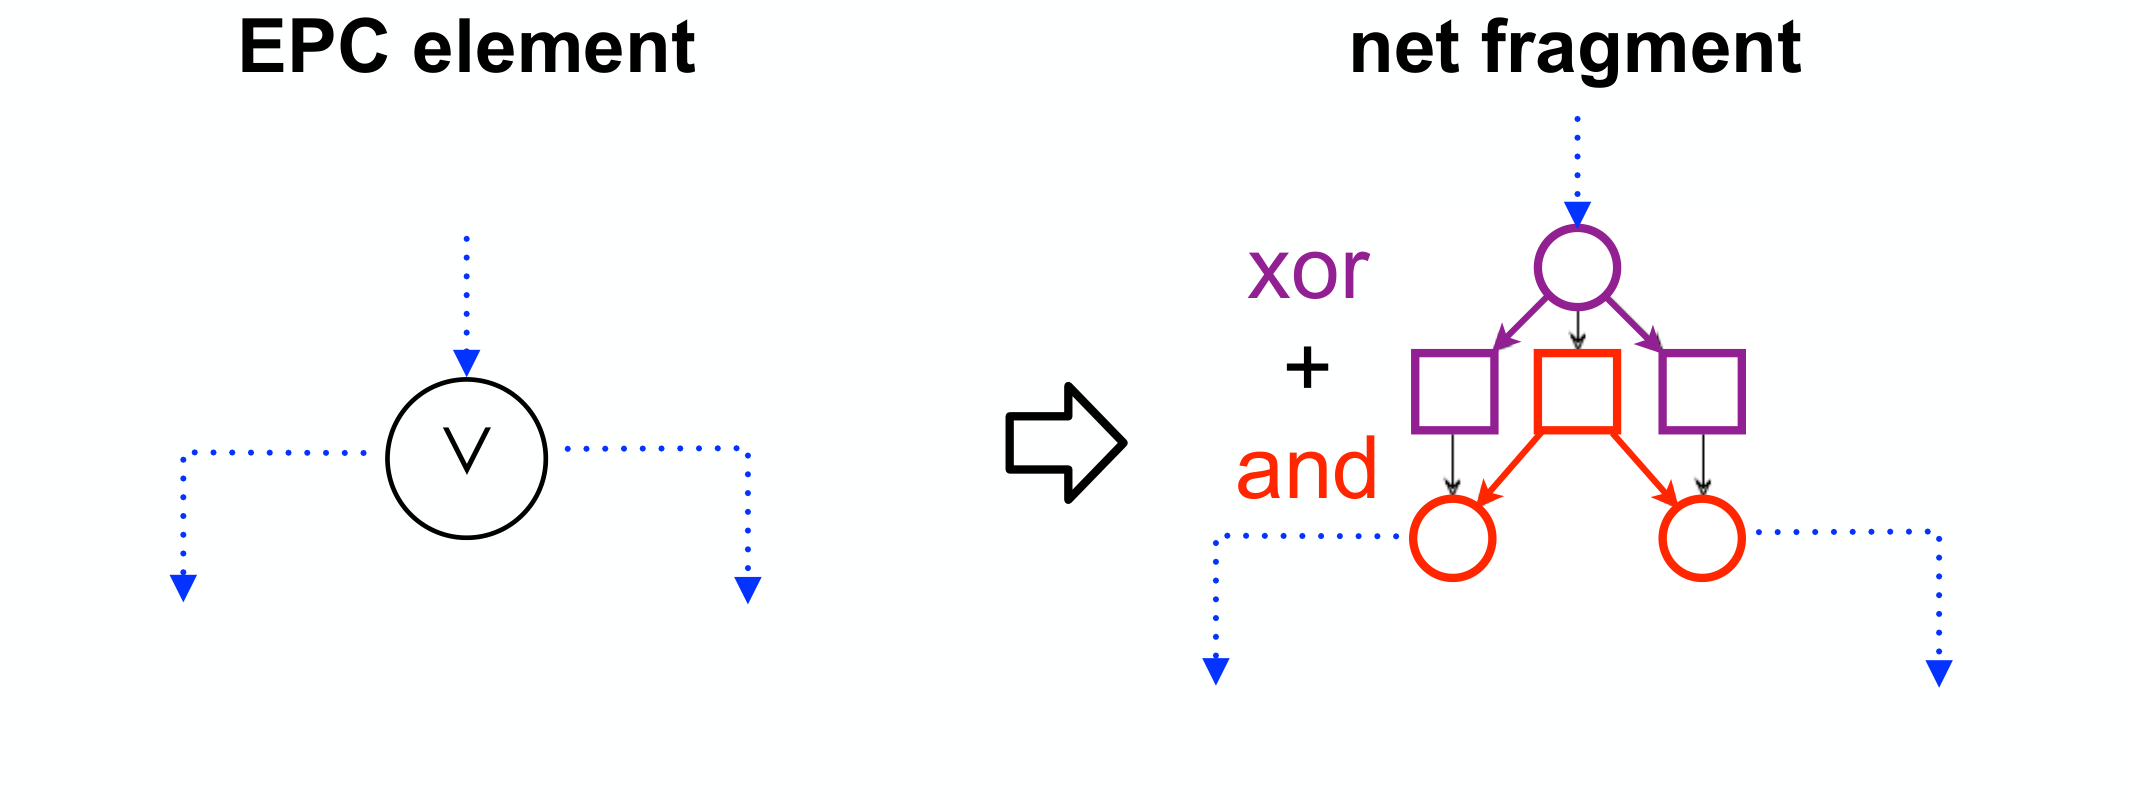
\includegraphics[width=0.74\linewidth,height=0.34\textheight,keepaspectratio]{images/16a-epc-analysis_p23_or-split.png}
\caption{Se il tuo EPC ha un OR-\textbf{split}, il frammento è: uno strato XOR che sceglie \textbf{quale sottoinsieme} di rami attivare, poi uno strato AND che li lancia tutti insieme.}
\end{figure}

\begin{figure}[!htb]
\centering
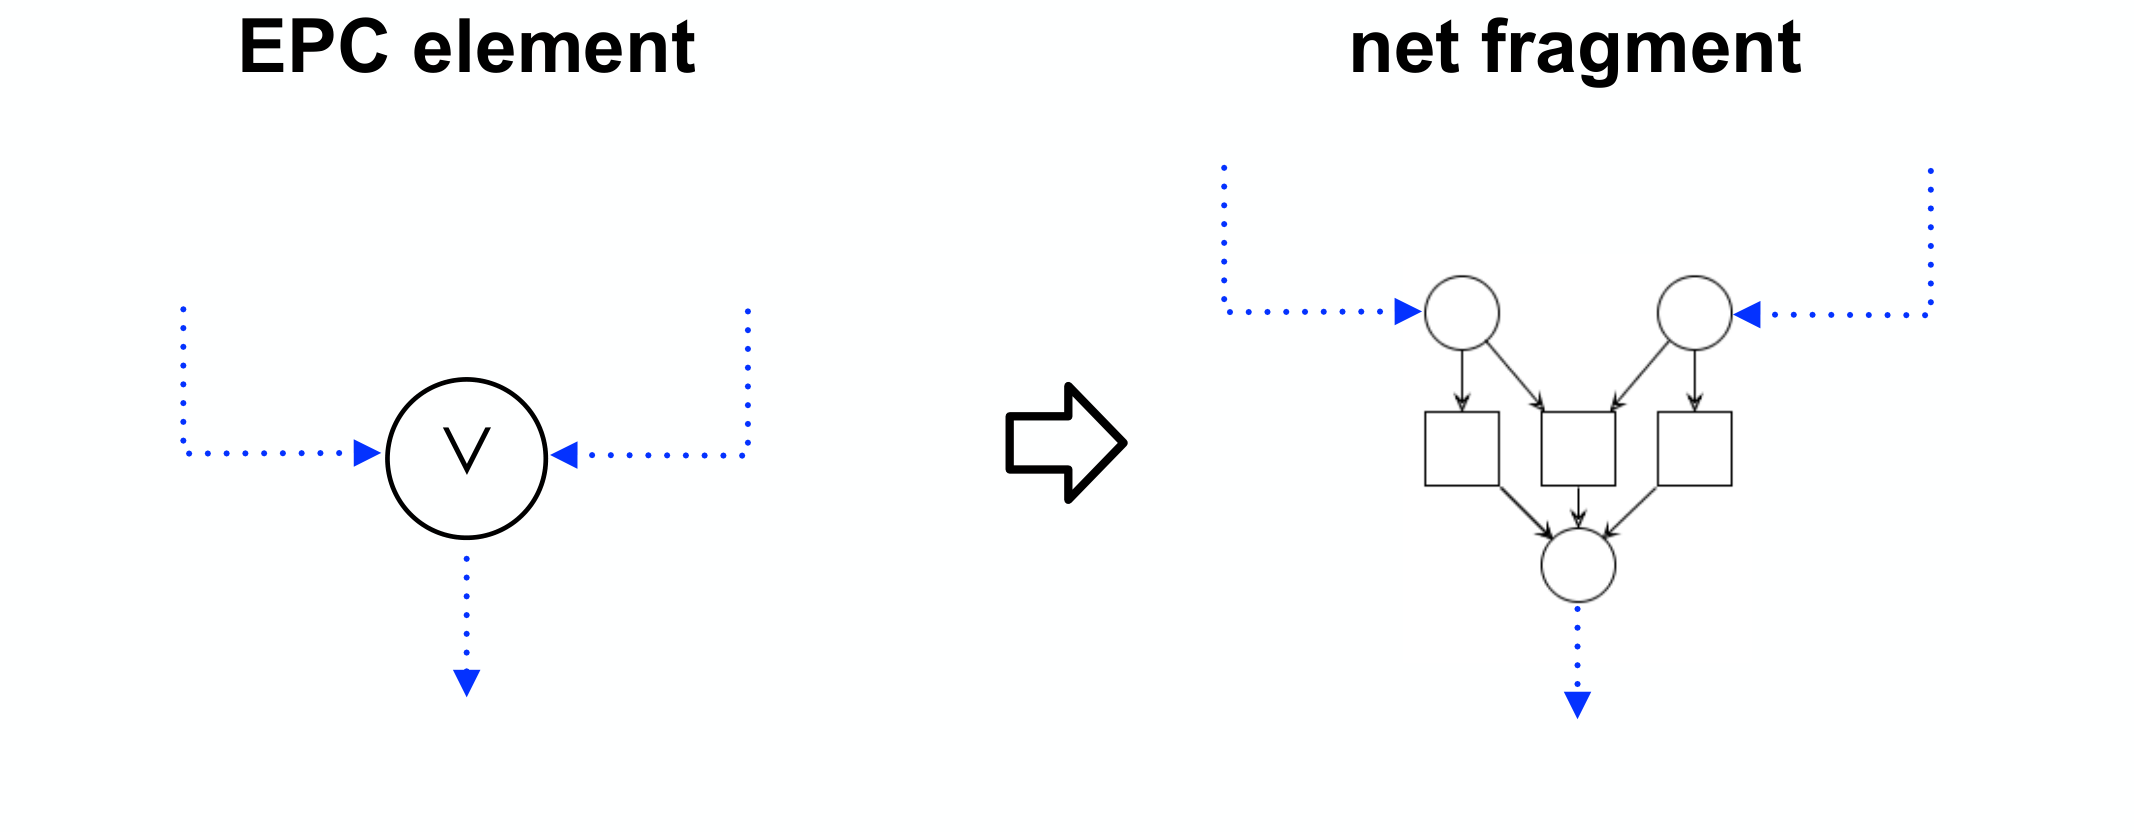
\includegraphics[width=0.74\linewidth,height=0.34\textheight,keepaspectratio]{images/16a-epc-analysis_p24_or-join.png}
\caption{L'OR-\textbf{join} duale: il frammento dovrebbe sincronizzare \emph{solo} i rami attivati — è il punto dove nascono le ambiguità (vedi la sezione "OR join" in \hyperref[ch:16a]{16a — EPC Analysis}).}
\end{figure}

\begin{boxexample}{Step 2 e 3 — connettere e chiudere}
\begin{itemize}
\item \textbf{Step 2}: dove due frammenti si toccano lasciando due place (o due transition) consecutivi, inserisci un \textbf{dummy} di raccordo (o \textbf{fondi} i due nodi, a seconda dello stile scelto).
\item \textbf{Step 3}: se ci sono più eventi di start (qui solo uno, "goods arrived") o più eventi finali, aggiungi un connettore XOR/AND/OR che li unifica in un solo place iniziale $i$ e uno finale $o$.
\end{itemize}
\end{boxexample}

\begin{figure}[!htb]
\centering
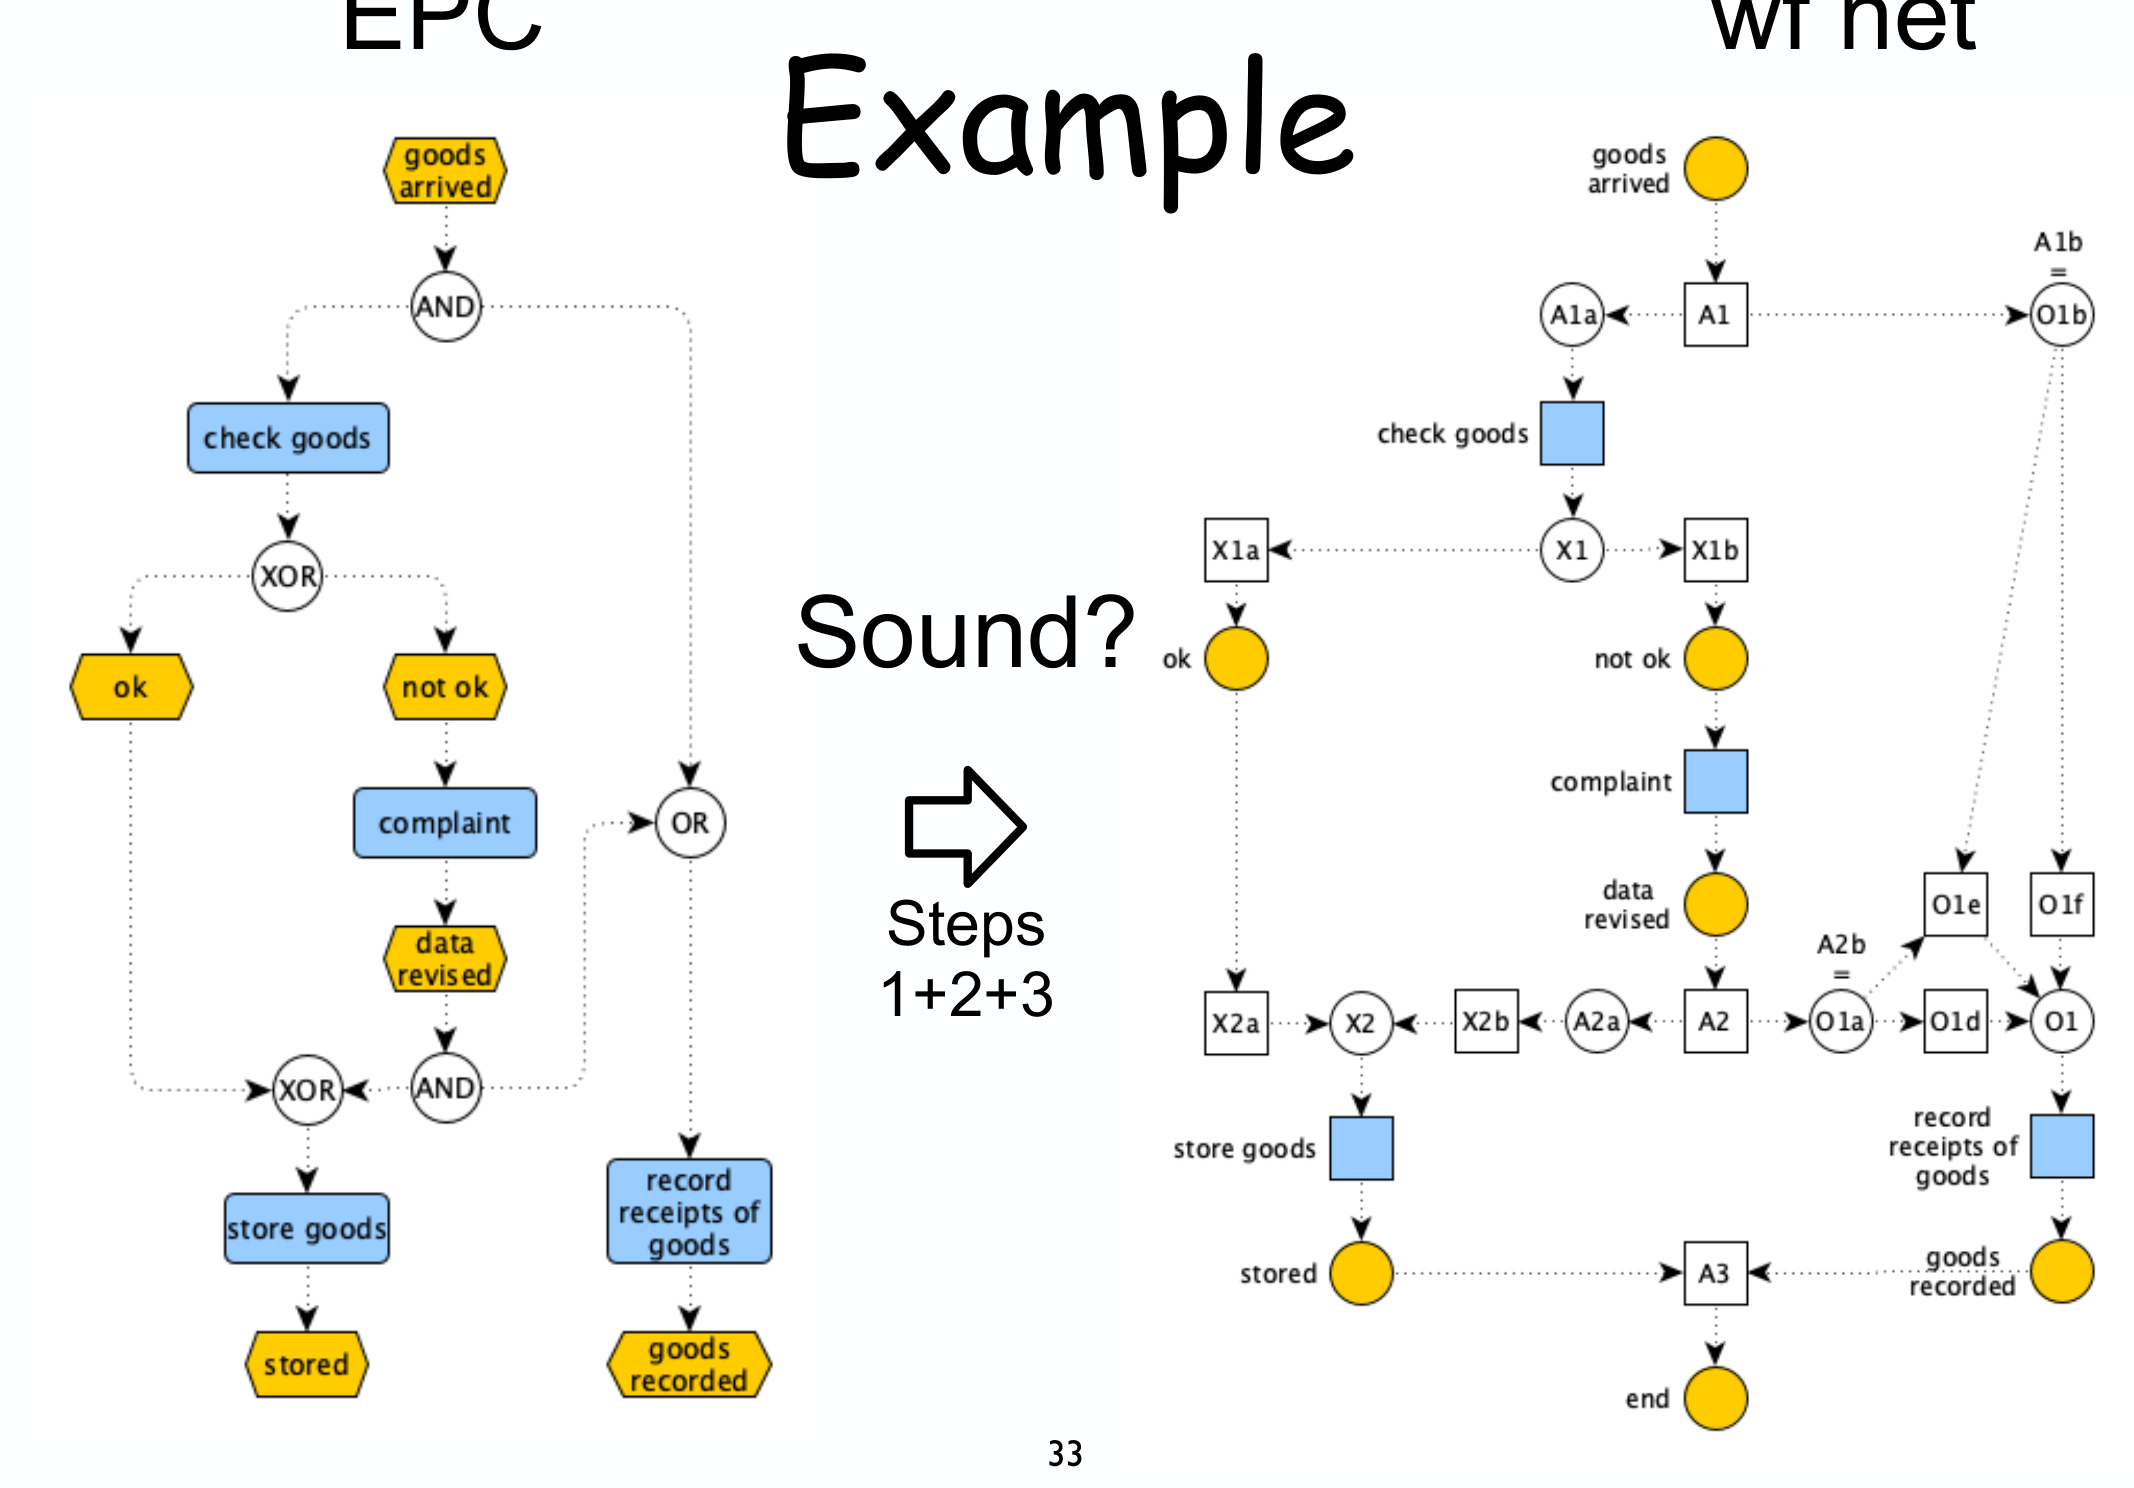
\includegraphics[width=0.74\linewidth,height=0.34\textheight,keepaspectratio]{images/16a-epc-analysis_p33_example-epc-wfnet.png}
\caption{Il prodotto finito dei tre step. Ora puoi applicare direttamente la sezione 5 (costruire $N^\star$ e leggerne il RG a colori) per rispondere a "è sound?". In questo caso specifico la risposta è \textbf{no}, proprio per colpa dell'OR-join (vedi \hyperref[ch:16a]{16a — EPC Analysis} per il perché).}
\end{figure}

\section{\texorpdfstring{7. Tradurre un BPMN in Petri net (il "twist")}{7. Tradurre un BPMN in Petri net (il "twist")}}

\emph{Teoria: \hyperref[ch:16b]{16b — BPMN Analysis}.}

Attenzione: nel BPMN la corrispondenza è \textbf{diversa} da quella EPC.

\begin{figure}[!htb]
\centering
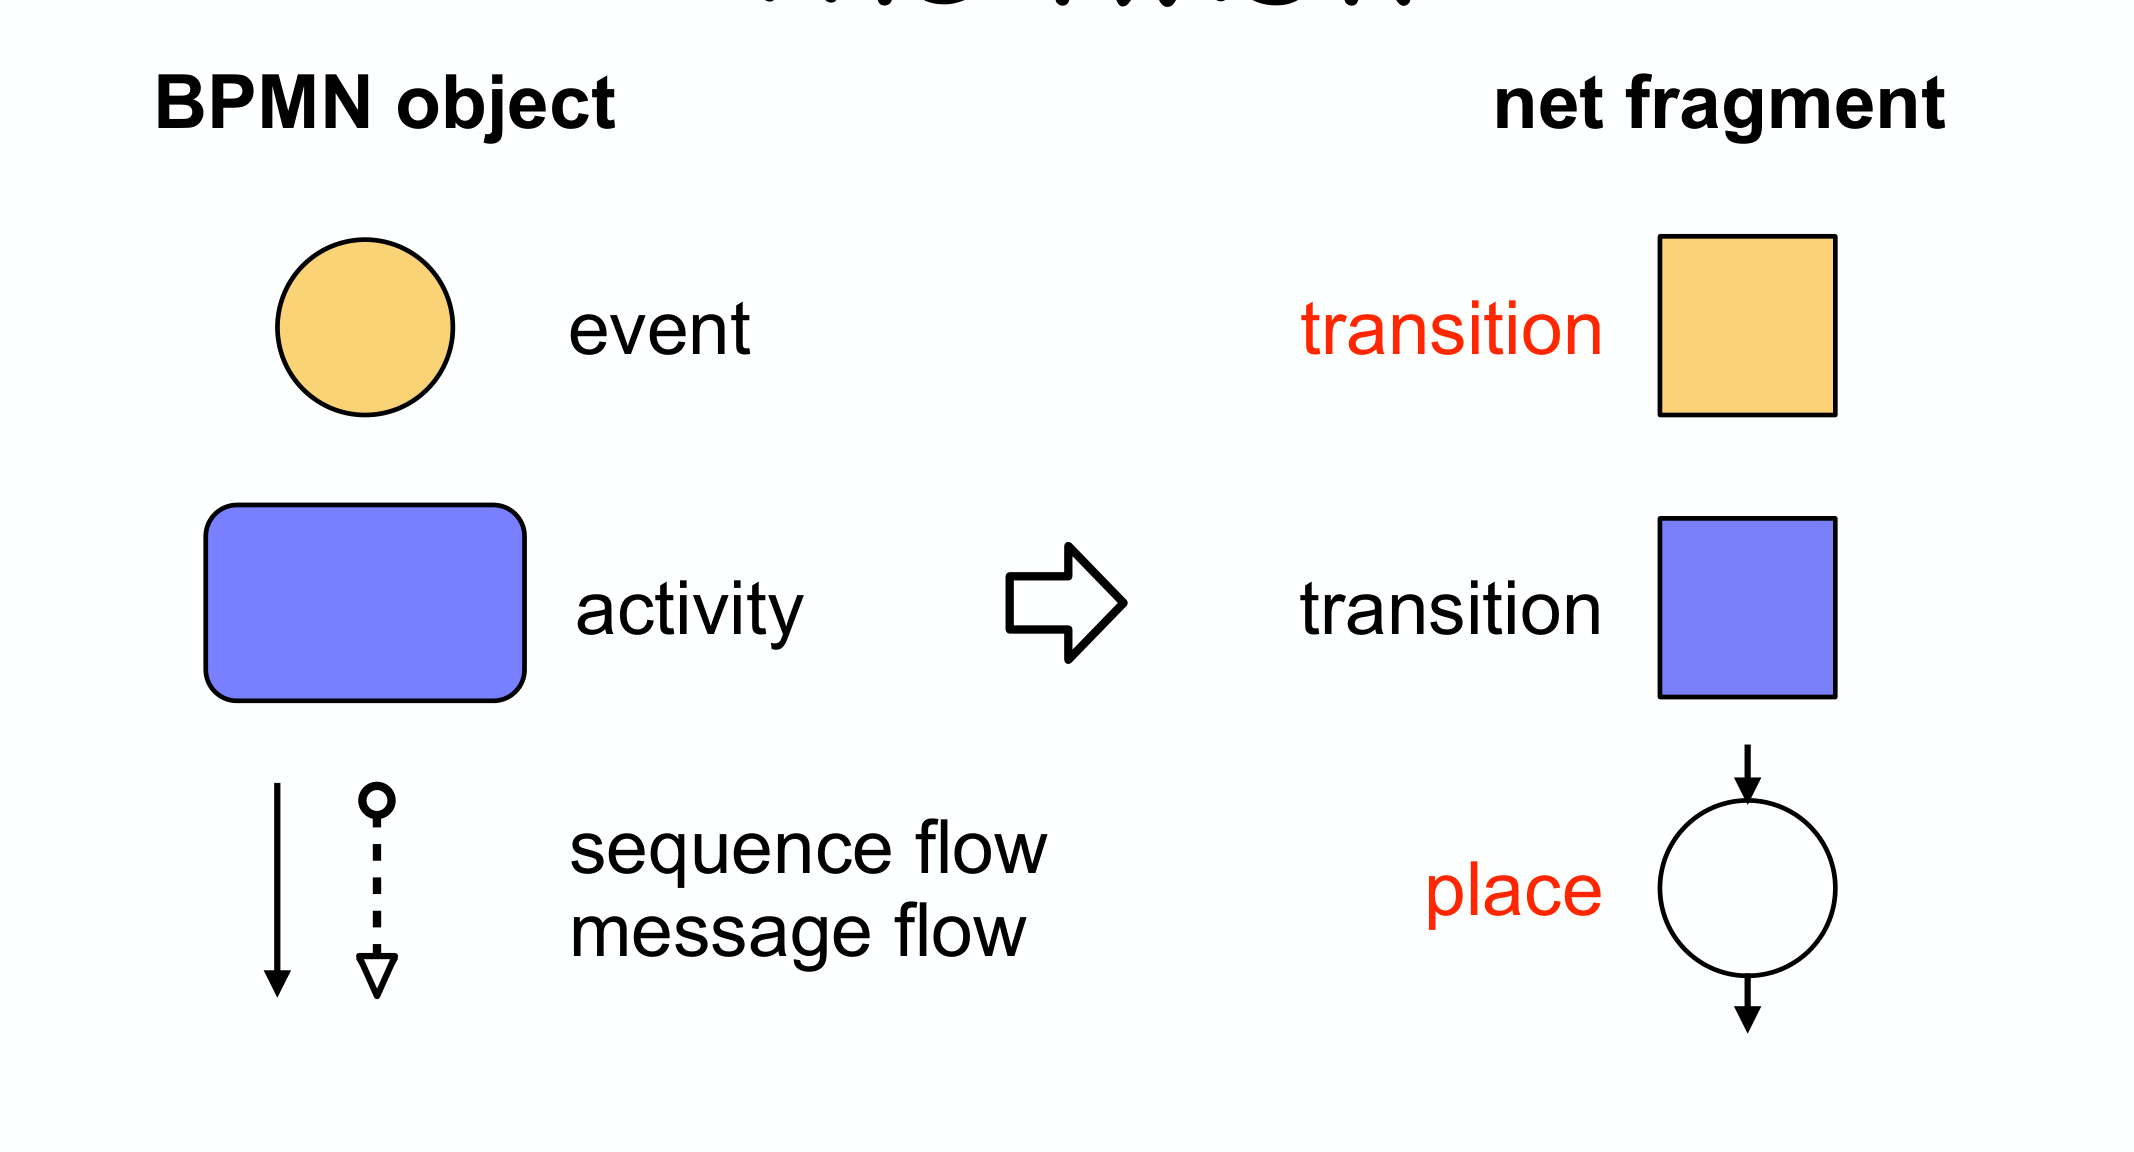
\includegraphics[width=0.74\linewidth,height=0.34\textheight,keepaspectratio]{images/16b-bpmn-analysis_p17_the-twist.png}
\caption{Da tenere sempre a mente prima di tradurre: \textbf{event} e \textbf{activity} $\rightarrow$ \textbf{transition}; gli \textbf{archi} (flow) $\rightarrow$ \textbf{place}. Il contrario dell'EPC.}
\end{figure}

Traduciamo l'\textbf{Order process}: un evento iniziale, un AND-split che avvia "check credit card" e "prepare products" in parallelo, poi uno XOR ok?/no che nel ramo "yes" passa per un AND-join con "ship products", mentre il ramo "no" salta direttamente alla fine.

\begin{figure}[!htb]
\centering
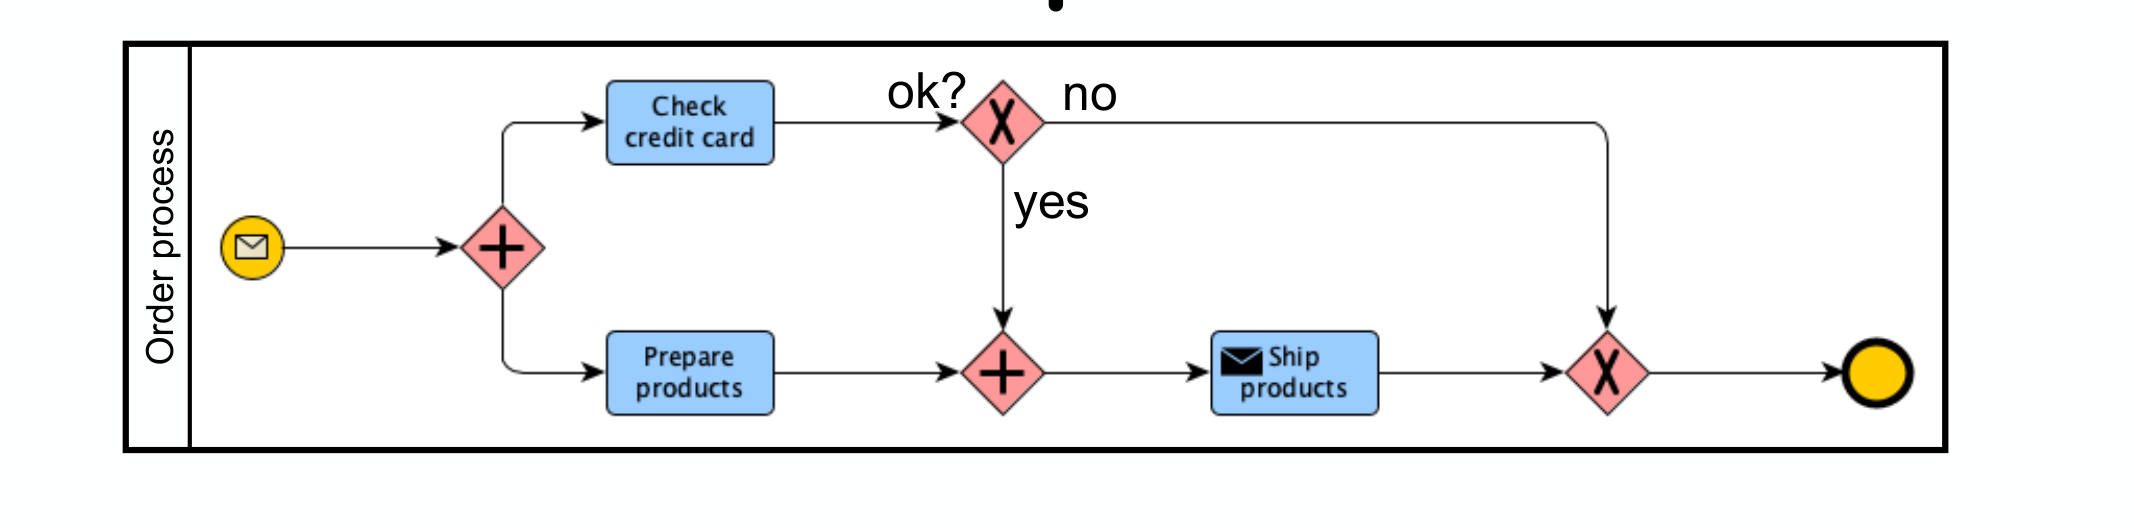
\includegraphics[width=0.74\linewidth,height=0.34\textheight,keepaspectratio]{images/16b-bpmn-analysis_p27_order-process.png}
\caption{Il diagramma da tradurre.}
\end{figure}

\begin{boxexample}{Applicare il twist passo-passo}
\begin{enumerate}
\item \textbf{Step 1 (flussi $\rightarrow$ place)}: metti un place su \textbf{ogni freccia} del diagramma (fra l'evento iniziale e l'AND-split, fra l'AND-split e ciascuna attività, ecc.).
\item \textbf{Step 2 (flow object $\rightarrow$ transition)}: metti una transition per l'evento iniziale, una per ciascuna attività, una per l'AND-split (con \textbf{due} output place, uno per ramo), una per l'AND-join (con \textbf{due} input place), due per lo XOR-split (una per il ramo "yes", una per il "no"), una per lo XOR-join.
\item \textbf{Step 3 (unico inizio/fine)}: qui c'è già un solo evento iniziale e uno finale, quindi non serve altro.
\end{enumerate}
\end{boxexample}

\begin{figure}[!htb]
\centering
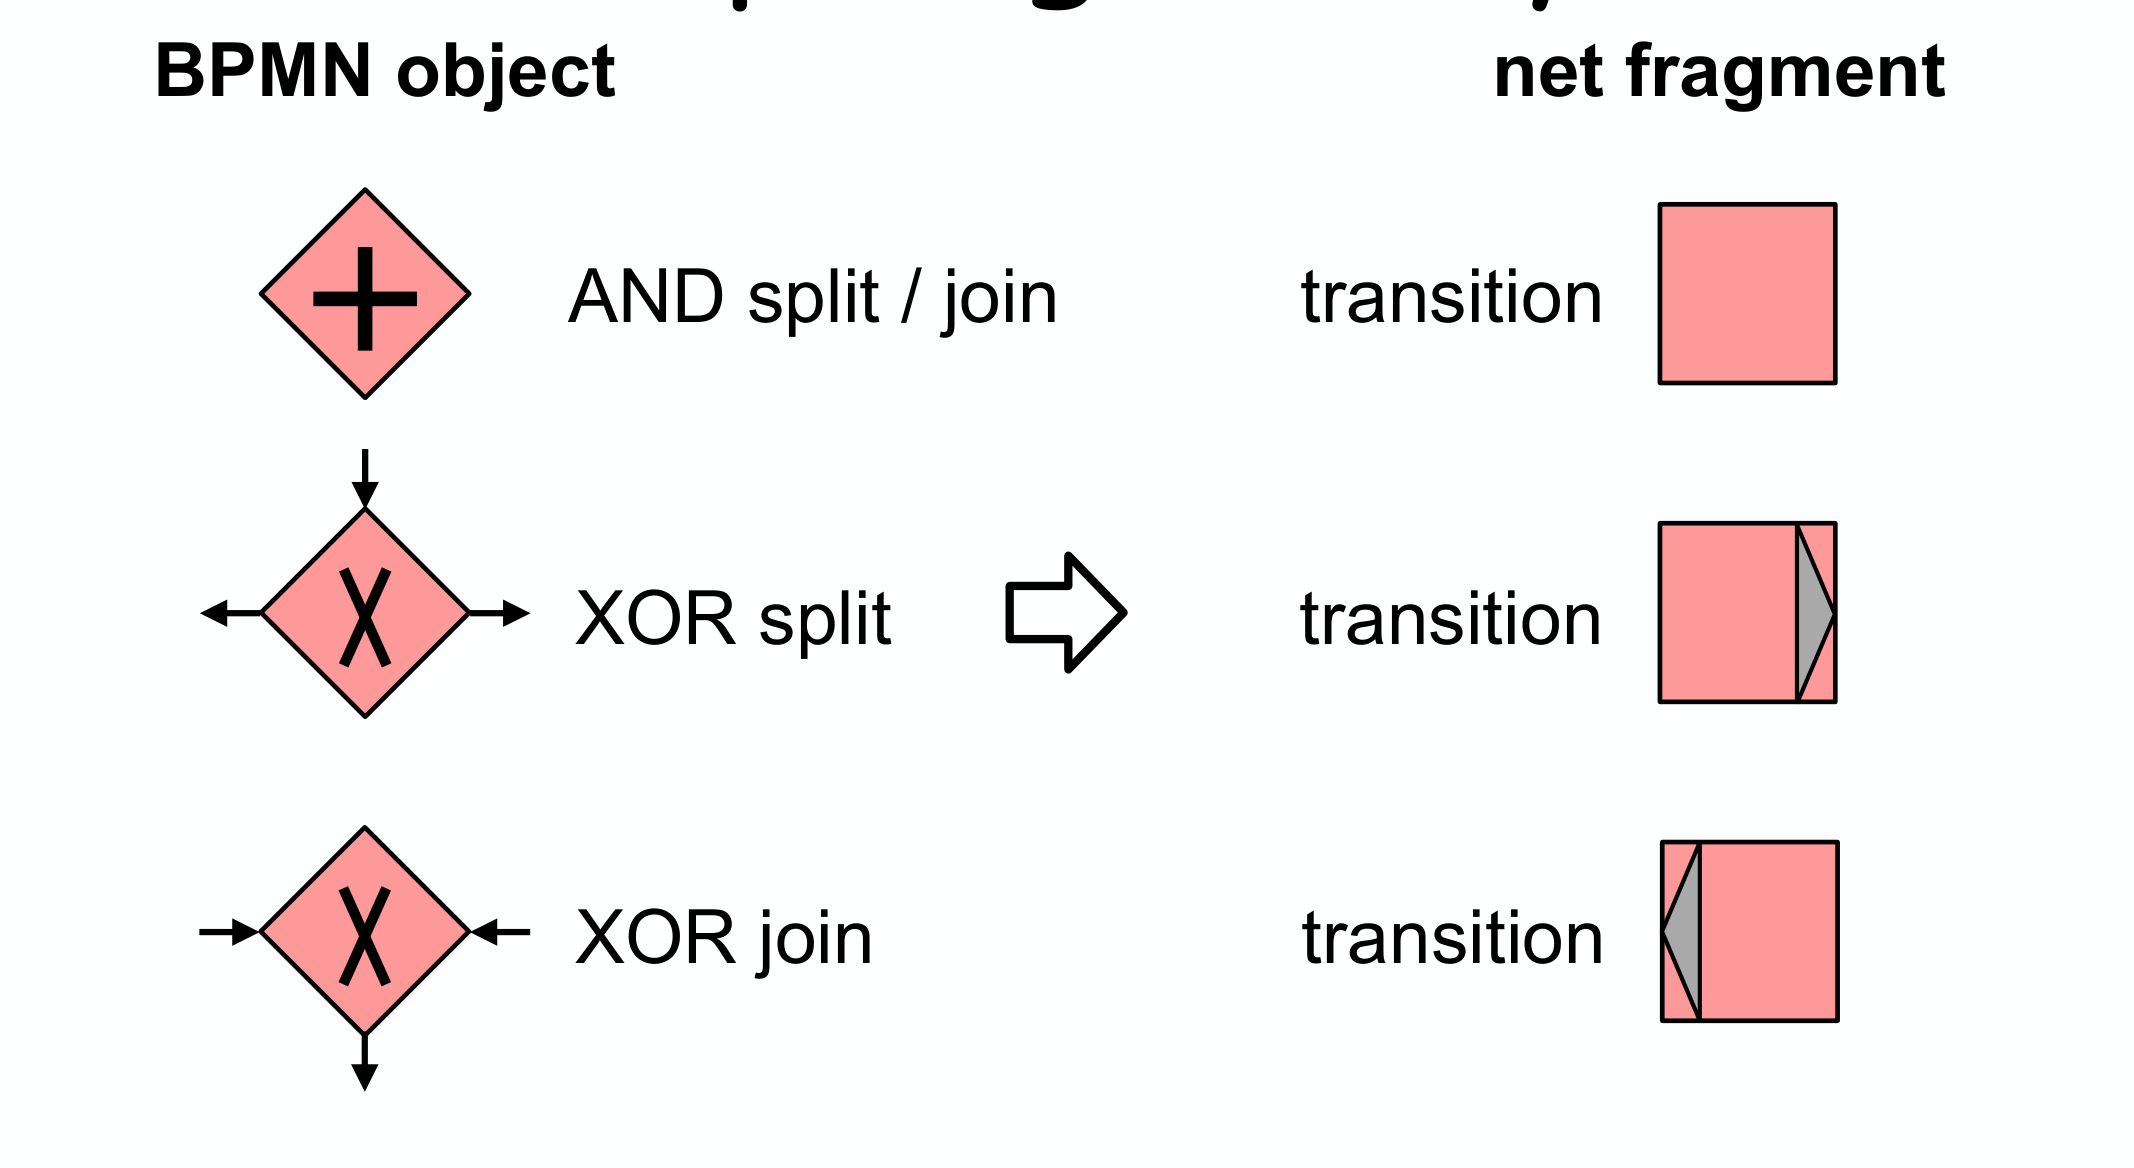
\includegraphics[width=0.74\linewidth,height=0.34\textheight,keepaspectratio]{images/16b-bpmn-analysis_p22_gateways.png}
\caption{Il frammento da usare per ciascun gateway nello Step 2.}
\end{figure}

\begin{boxwarning}{Il difetto, visibile già nella traduzione}
L'AND-split lancia \textbf{due} token (uno per "check credit card", uno per "prepare products"). Il ramo "no" dello XOR-join, però, \textbf{non aspetta} l'altro ramo prima di andare alla fine: risultato, un token del ramo "prepare products" resta \textbf{pendente} nella rete (proper completion violata) — esattamente il difetto "mismatch AND/XOR" spiegato in \hyperref[ch:16b]{16b — BPMN Analysis}. Costruendo $N^\star$ e il suo RG (sezione 5) lo si vede subito come non-live/non-bounded.
\end{boxwarning}

\section{\texorpdfstring{8. Free-choice, siphon, trap: applicare il teorema di Commoner}{8. Free-choice, siphon, trap: applicare il teorema di Commoner}}

\emph{Teoria: \hyperref[ch:17]{17 — Free Choice}.}

\subsection{\texorpdfstring{Passo 1 — verificare la proprietà free-choice}{Passo 1 — verificare la proprietà free-choice}}

\begin{boxexample}{Controllo diretto sui pre-set}
Regola: per ogni coppia di transition,

\[
\bullet t_1 \cap \bullet t_2 = \emptyset \qquad\text{oppure}\qquad \bullet t_1 = \bullet t_2
\]
\end{boxexample}

\begin{figure}[!htb]
\centering
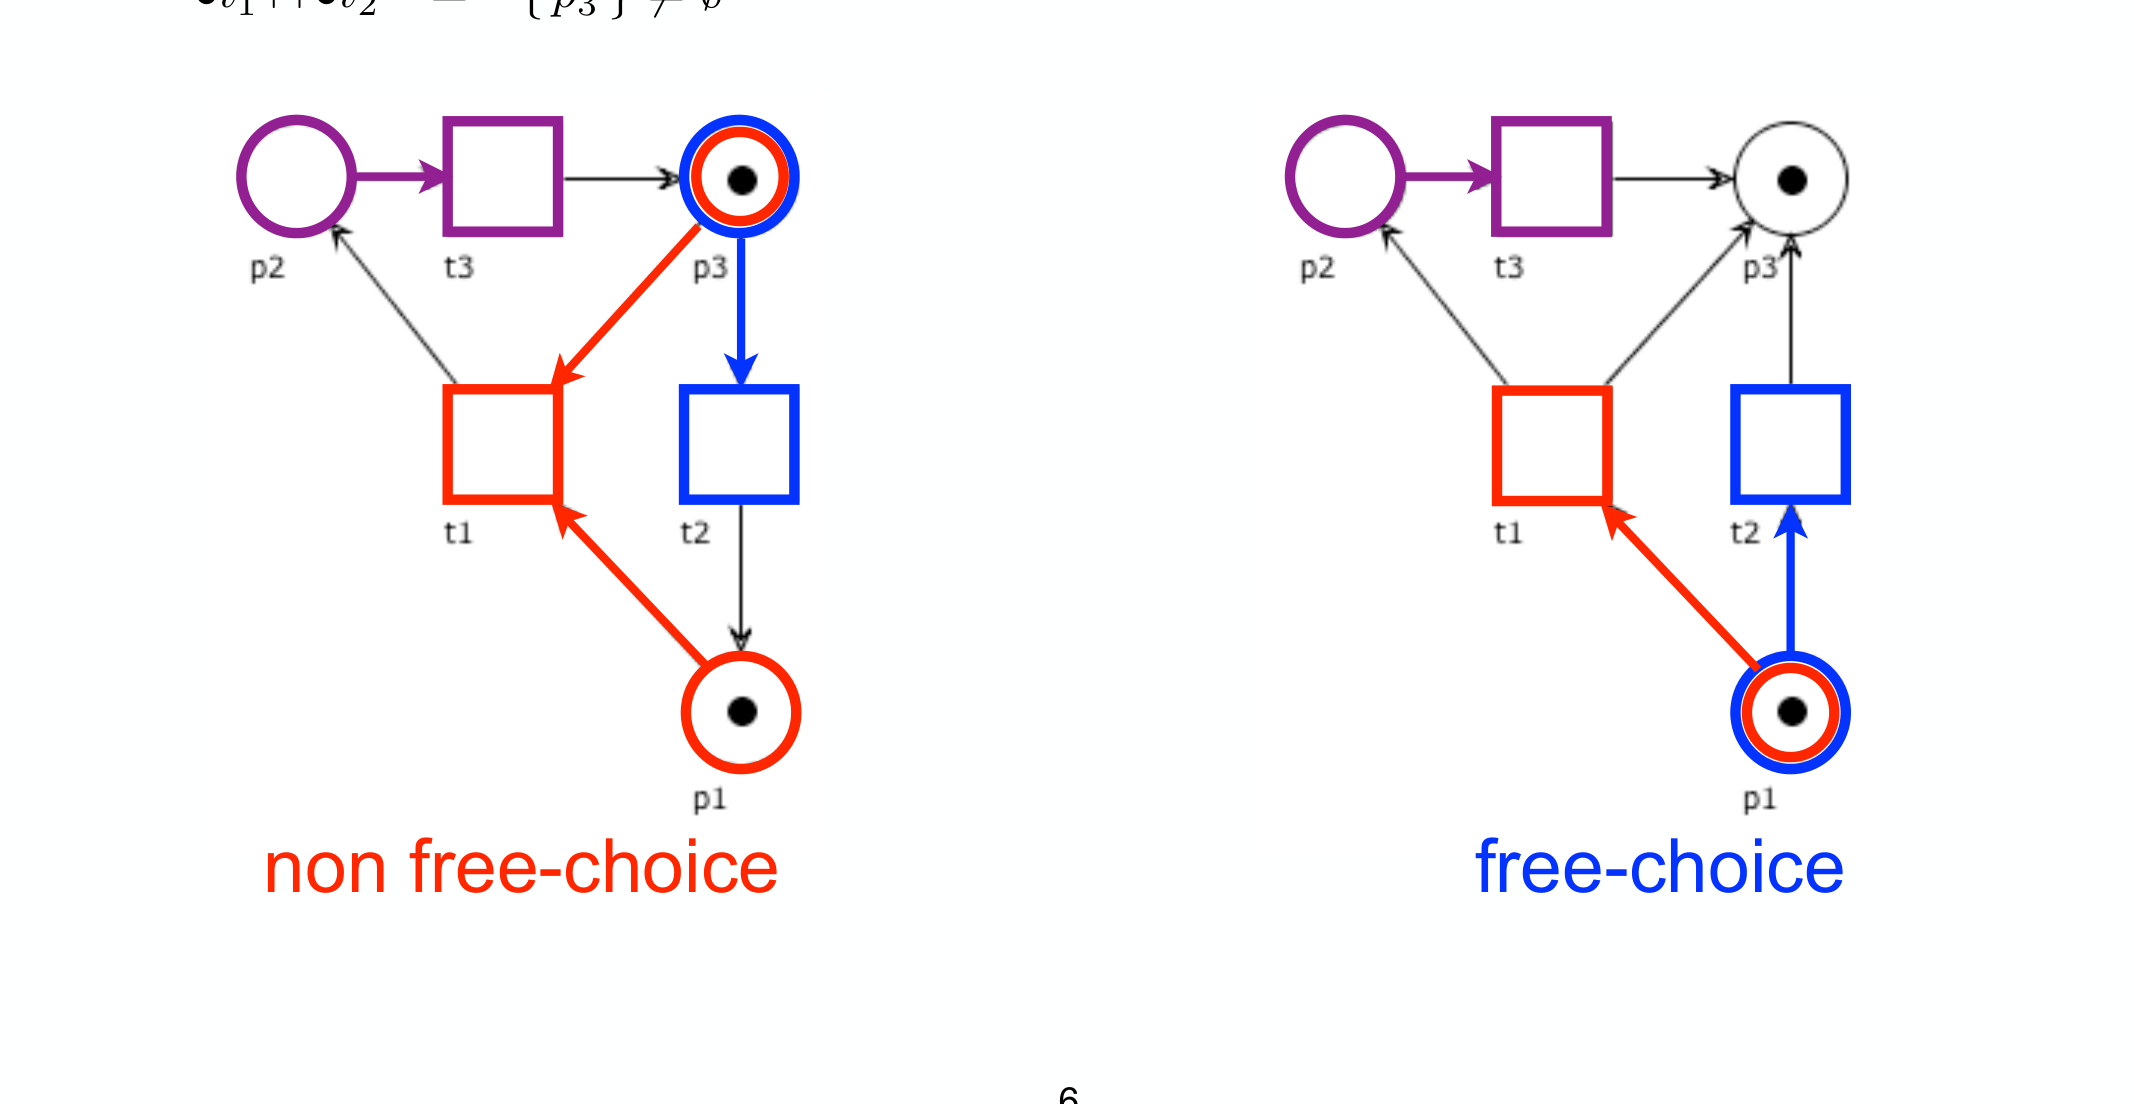
\includegraphics[width=0.74\linewidth,height=0.34\textheight,keepaspectratio]{images/17-free-choice_p6_fc-vs-nonfc.png}
\caption{A sinistra: $\bullet t_1=\{p_1,p_3\}$, $\bullet t_2=\{p_3\}$. L'intersezione è $\{p_3\}\ne\emptyset$ ma $\bullet t_1\ne\bullet t_2$ $\rightarrow$ \textbf{non} free-choice. A destra: $\bullet t_1=\bullet t_2$ (uguali) e $\bullet t_3$ è disgiunto da entrambi $\rightarrow$ free-choice.}
\end{figure}

\subsection{\texorpdfstring{Passo 2 — trovare un siphon (e verificarlo)}{Passo 2 — trovare un siphon (e verificarlo)}}

Sulla rete produttore/consumatore, candidato:

\[
R=\{\text{prod1busy},\ \text{prod1free},\ \text{itembuffer}\}
\]

Si controlla:

\[
\bullet R \subseteq R\bullet
\]

(ogni transition che \emph{entra} in $R$ deve essere coperta da quelle che \emph{escono}).

\begin{figure}[!htb]
\centering
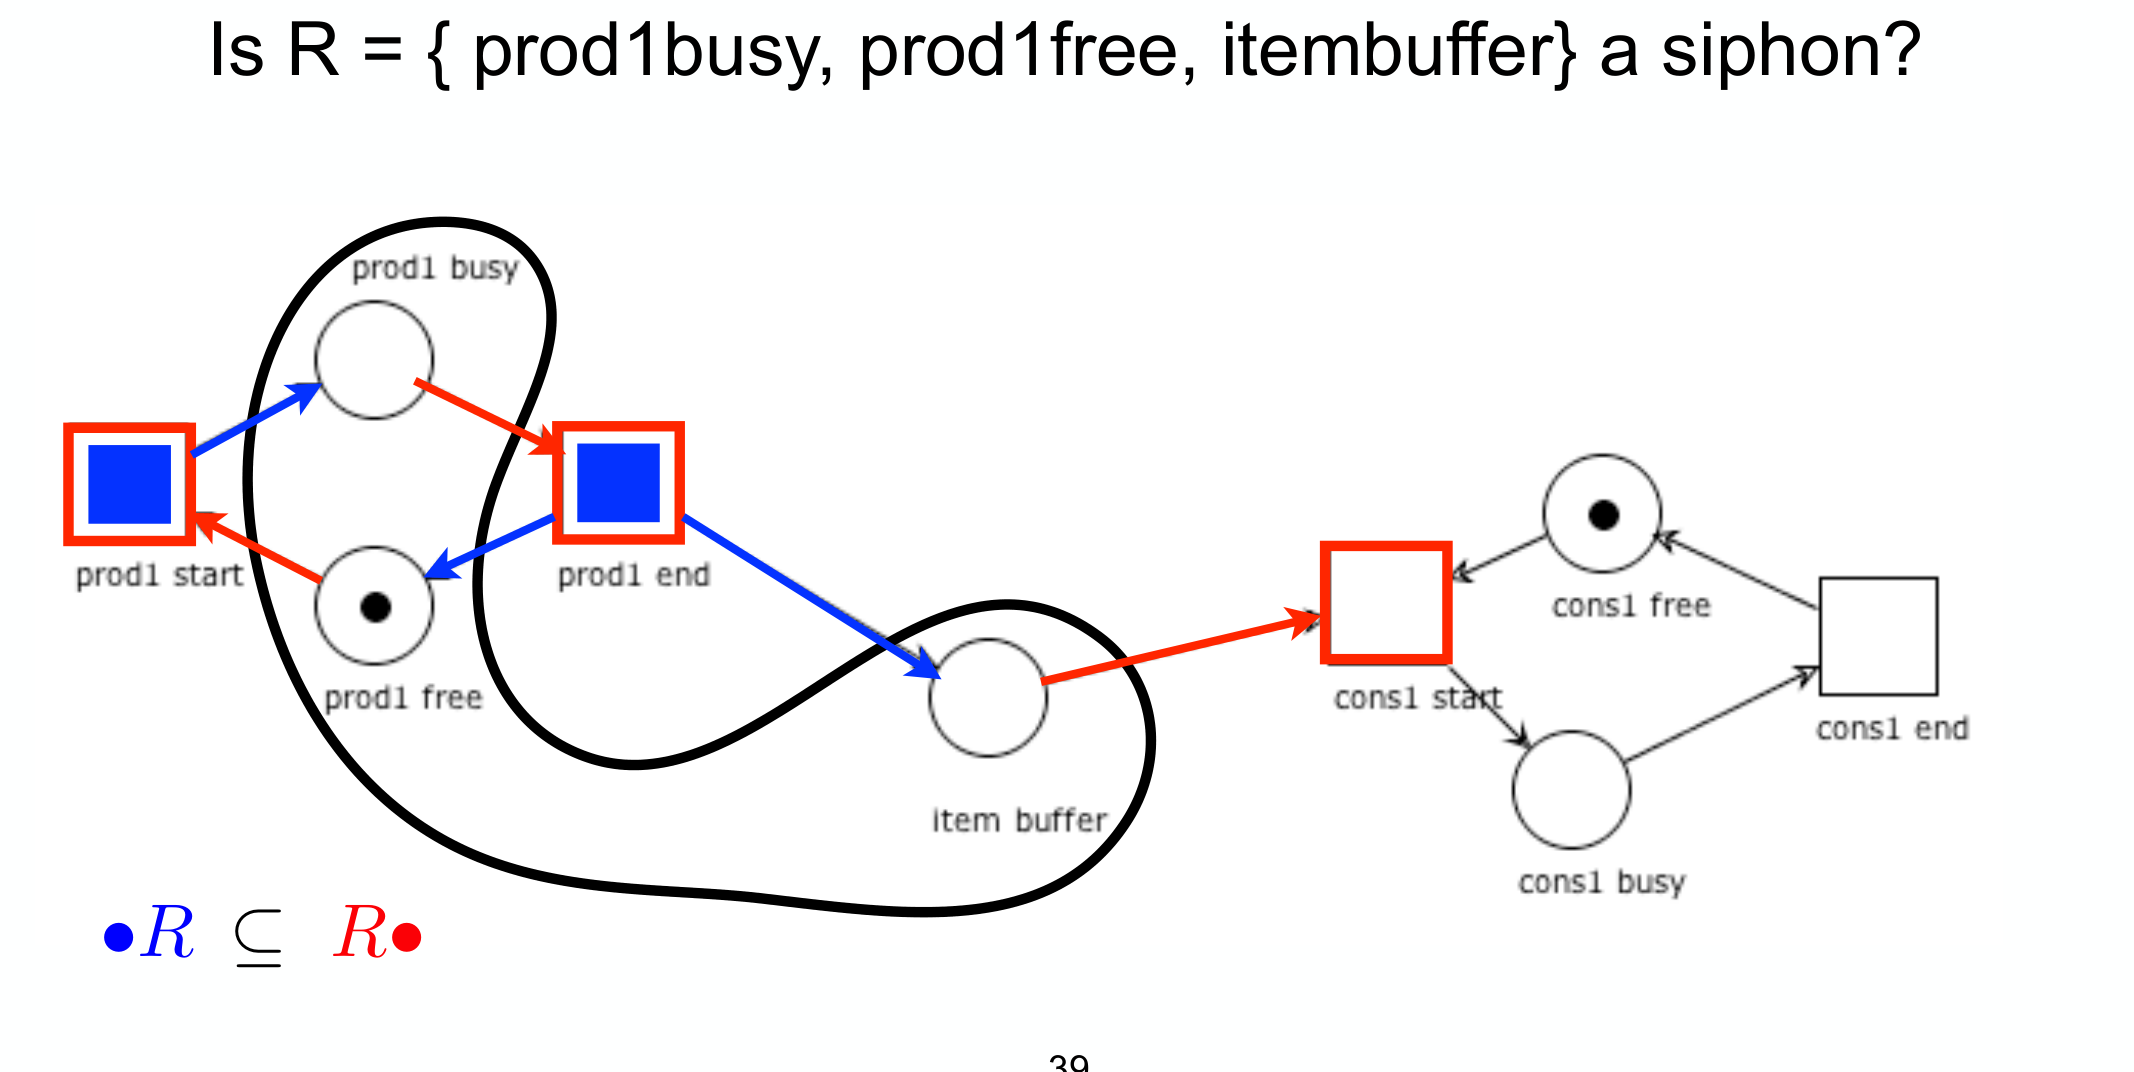
\includegraphics[width=0.74\linewidth,height=0.34\textheight,keepaspectratio]{images/17-free-choice_p39_siphon-check.png}
\caption{Ogni transition blu ($\bullet R$) coincide con una rossa ($R\bullet$): \textbf{sì}, $R$ è un siphon. Se restasse vuoto, non riceverebbe mai più token.}
\end{figure}

\subsection{\texorpdfstring{Passo 3 — trovare un trap che lo "salva"}{Passo 3 — trovare un trap che lo "salva"}}

Se $R$ contenesse un \textbf{trap} inizialmente marcato, per il teorema di Commoner la liveness sarebbe salva su quel fronte. Proviamo prima un candidato troppo piccolo, poi quello giusto:

\begin{figure}[!htb]
\centering
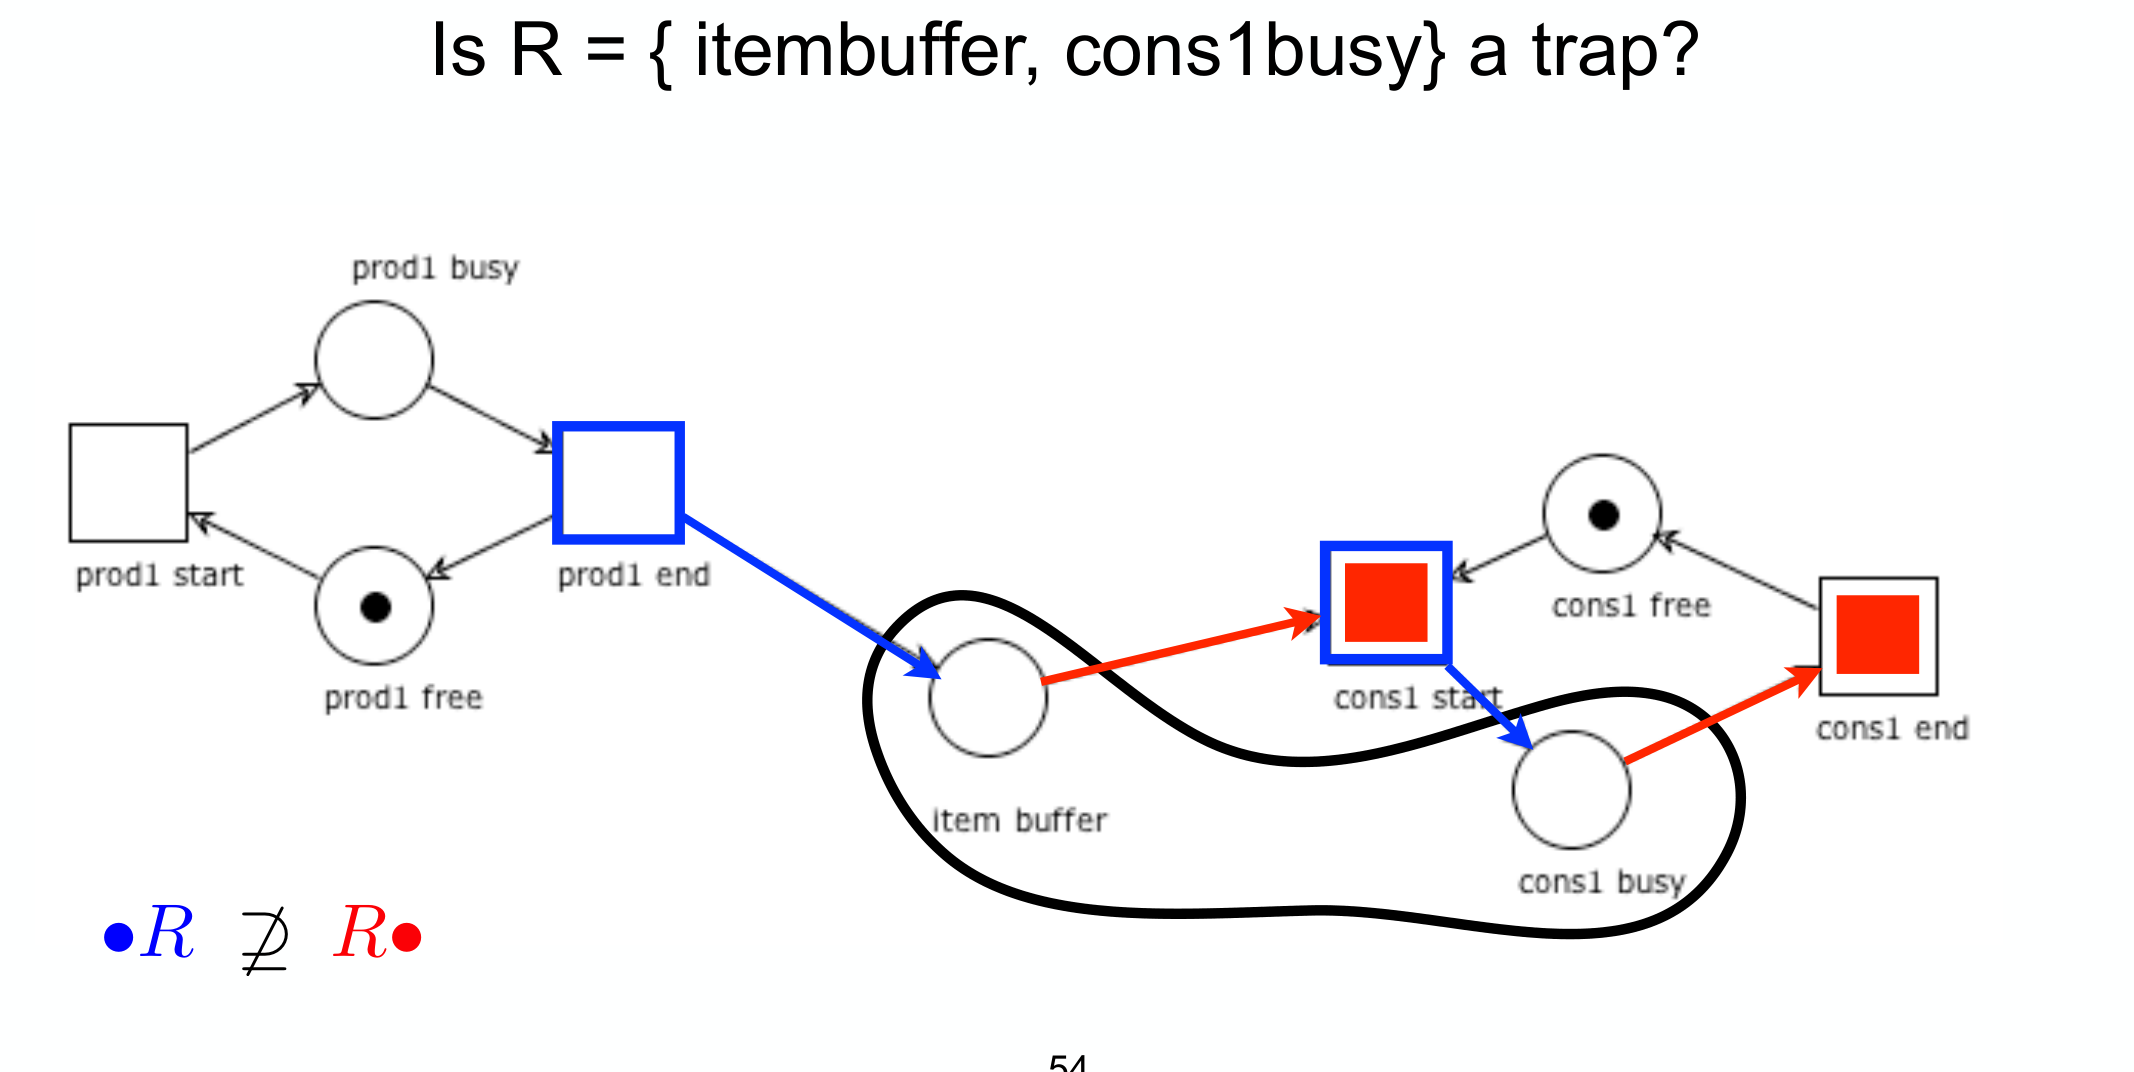
\includegraphics[width=0.74\linewidth,height=0.34\textheight,keepaspectratio]{images/17-free-choice_p54_trap-check.png}
\caption{Con $R=\{\text{itembuffer},\text{cons1busy}\}$: $R\bullet \not\subseteq \bullet R$ $\rightarrow$ \textbf{non} è un trap (manca un pezzo).}
\end{figure}

\begin{figure}[!htb]
\centering
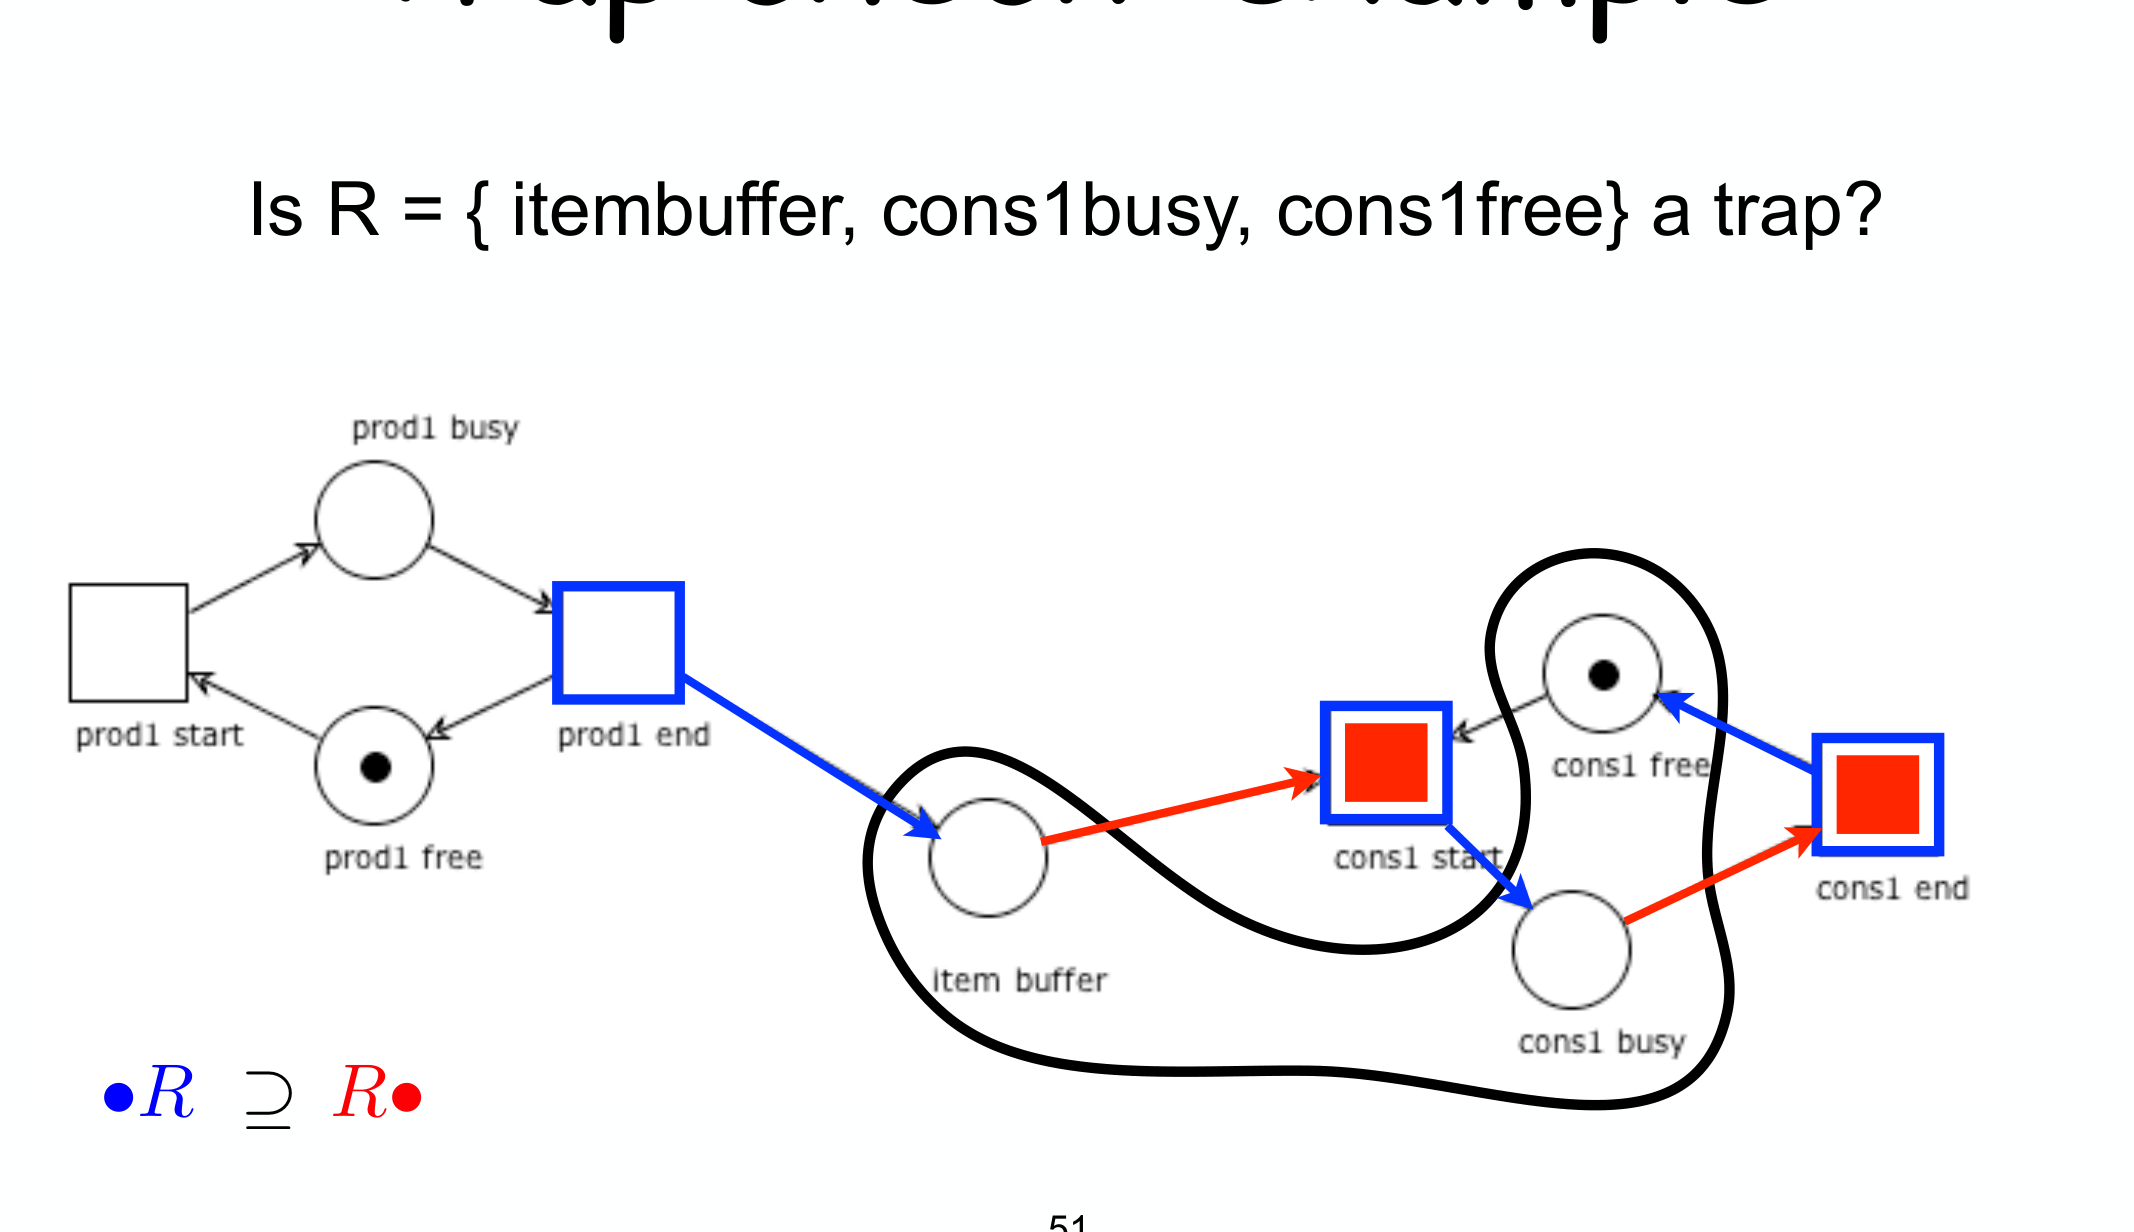
\includegraphics[width=0.74\linewidth,height=0.34\textheight,keepaspectratio]{images/22-esercizi_p51_trap-valid.png}
\caption{Allargando a $R=\{\text{itembuffer},\text{cons1busy},\text{cons1free}\}$: ora $R\bullet \subseteq \bullet R$ $\rightarrow$ \textbf{è un trap}. Se è marcato in $M_0$ (basta un token in uno dei tre place), il teorema di Commoner garantisce che questo particolare siphon \textbf{non condanna} la liveness.}
\end{figure}

\begin{boxtip}{Il procedimento generale}
\begin{enumerate}
\item Trova un siphon non ovviamente marcato (candidato "sospetto").
\item Cerca il \textbf{trap massimale} contenuto in quel siphon (si parte dal siphon e si tolgono i place che rompono la condizione di trap, come nel passaggio sopra).
\item Se il trap massimale è \textbf{marcato} in $M_0$ $\rightarrow$ quel siphon non è un problema. Se \textbf{tutti} i proper siphon superano questo test $\rightarrow$ la rete free-choice è \textbf{live} (Commoner).
\end{enumerate}
\end{boxtip}

\section{\texorpdfstring{9. Comporre due workflow module in un workflow system}{9. Comporre due workflow module in un workflow system}}

\emph{Teoria: \hyperref[ch:18]{18 — Workflow Systems}.}

\begin{boxexample}{Passo 1 — costruire l'interfaccia di un modulo}
Il process \textbf{Seller} riceve un suggerimento (\texttt{?rec\_accept}/\texttt{?rec\_reject}) e invia una decisione (\texttt{!accept}/\texttt{!reject}). Le sue attività di ricezione/invio diventano \textbf{place di interfaccia}.
\end{boxexample}

\begin{figure}[!htb]
\centering
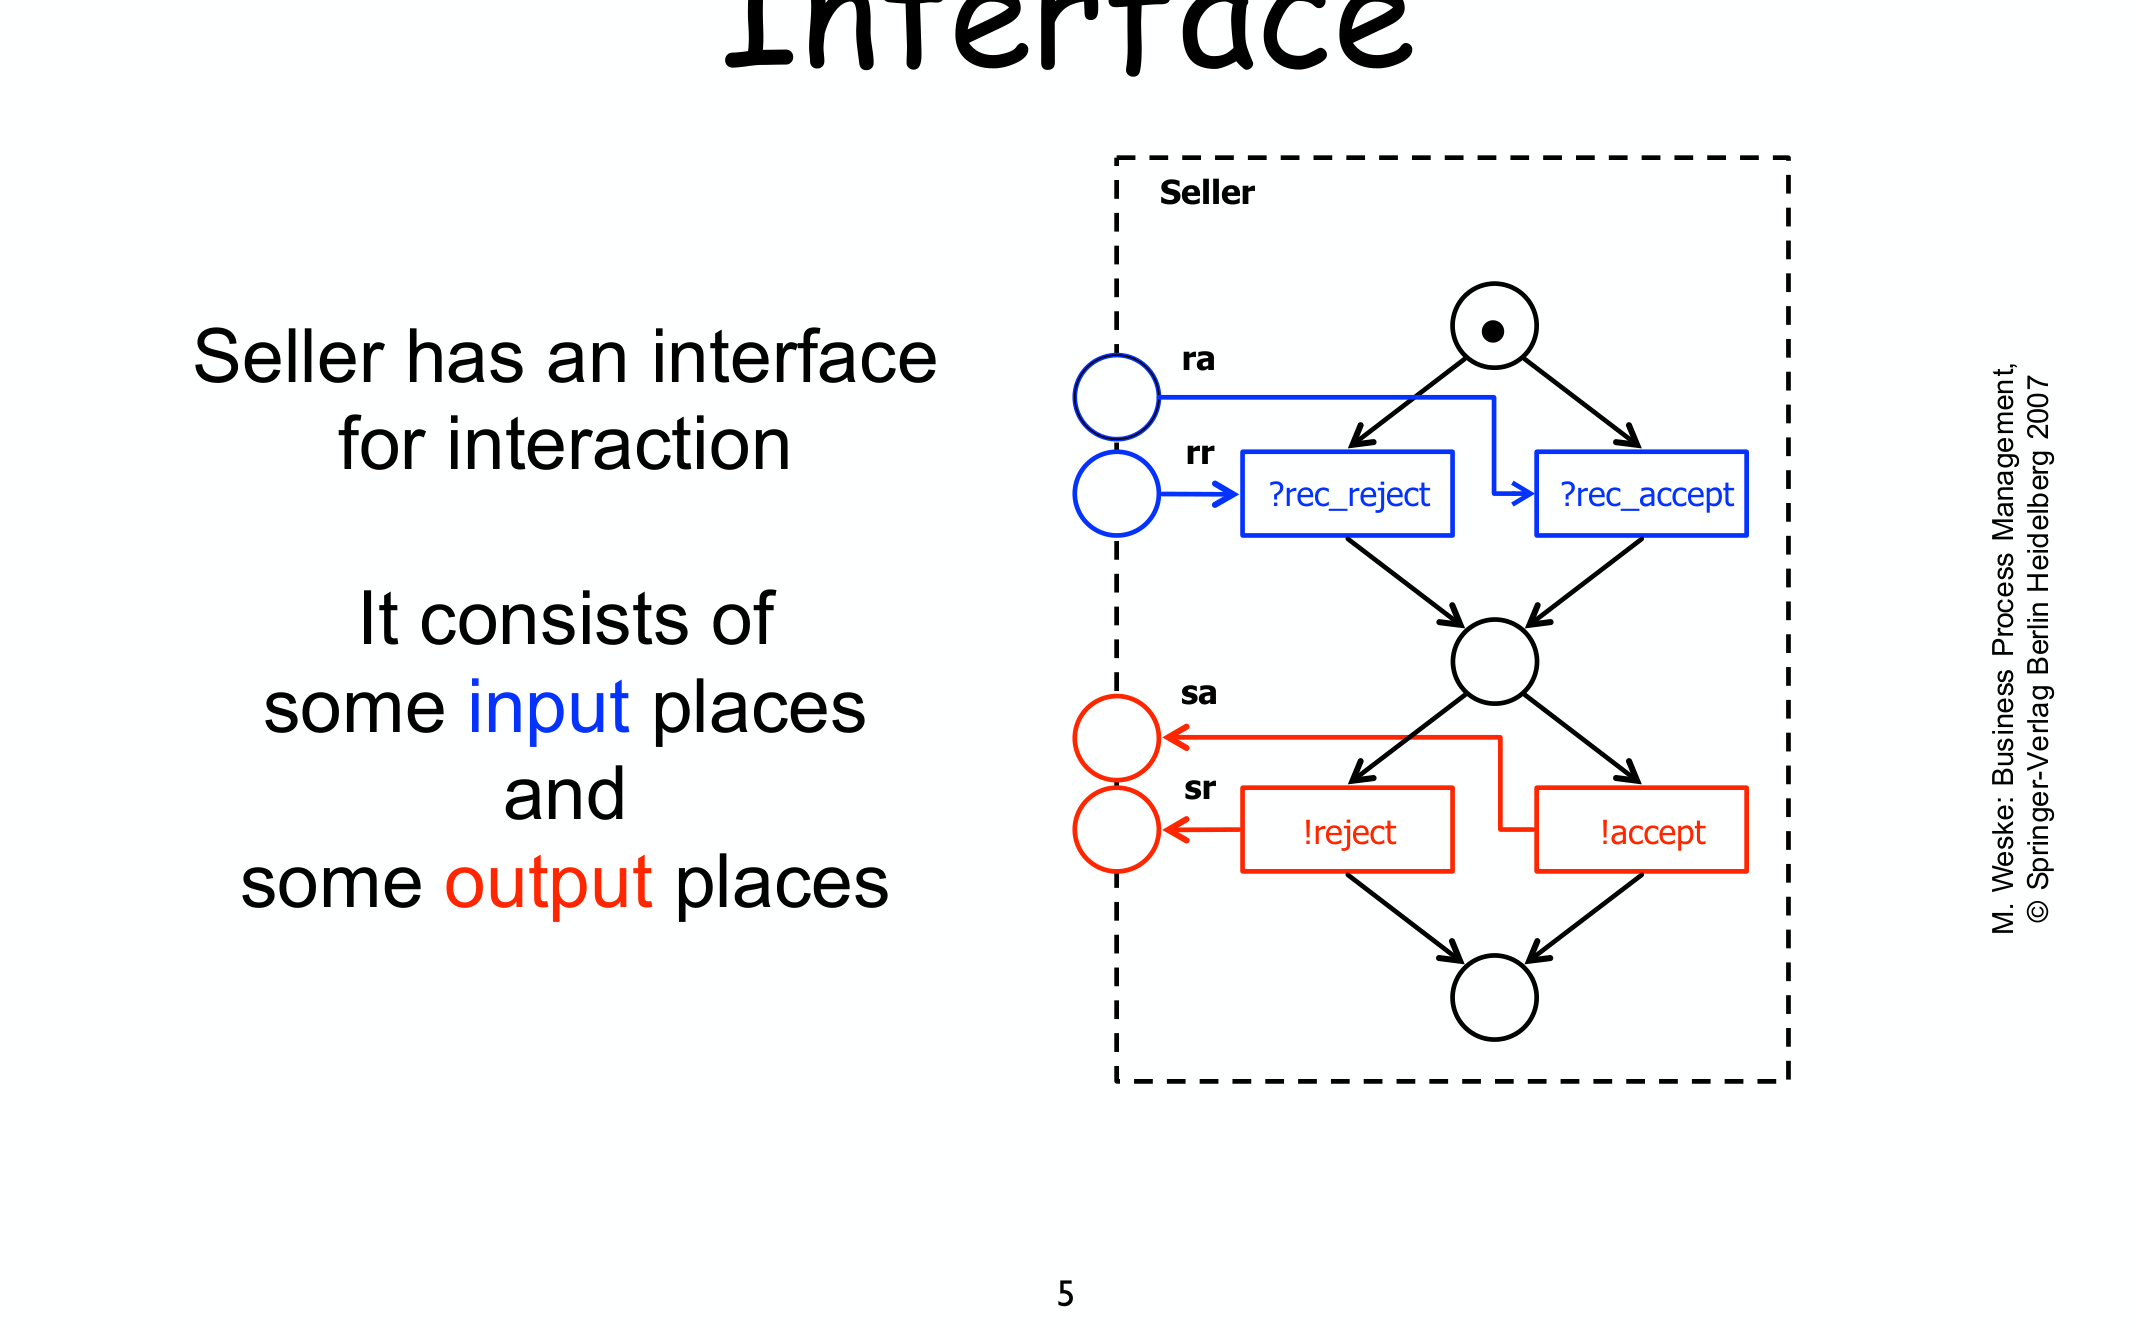
\includegraphics[width=0.74\linewidth,height=0.34\textheight,keepaspectratio]{images/18-workflow-systems_p5_interface.png}
\caption{$P_I=\{ra,rr\}$ alimentano \texttt{?rec\_reject}/\texttt{?rec\_accept}; $P_O=\{sa,sr\}$ sono riempiti da \texttt{!reject}/\texttt{!accept}.}
\end{figure}

\begin{boxexample}{Passo 2 — verificare compatibilità e comporre}
\textbf{Auctioning Service} invia su \texttt{ra}/\texttt{rr} esattamente ciò che Seller riceve, e viceversa su \texttt{sa}/\texttt{sr}: sono \textbf{structurally compatible}. Si compongono \textbf{fondendo} i place di interfaccia condivisi (nessuna transition aggiuntiva).
\end{boxexample}

\begin{figure}[!htb]
\centering
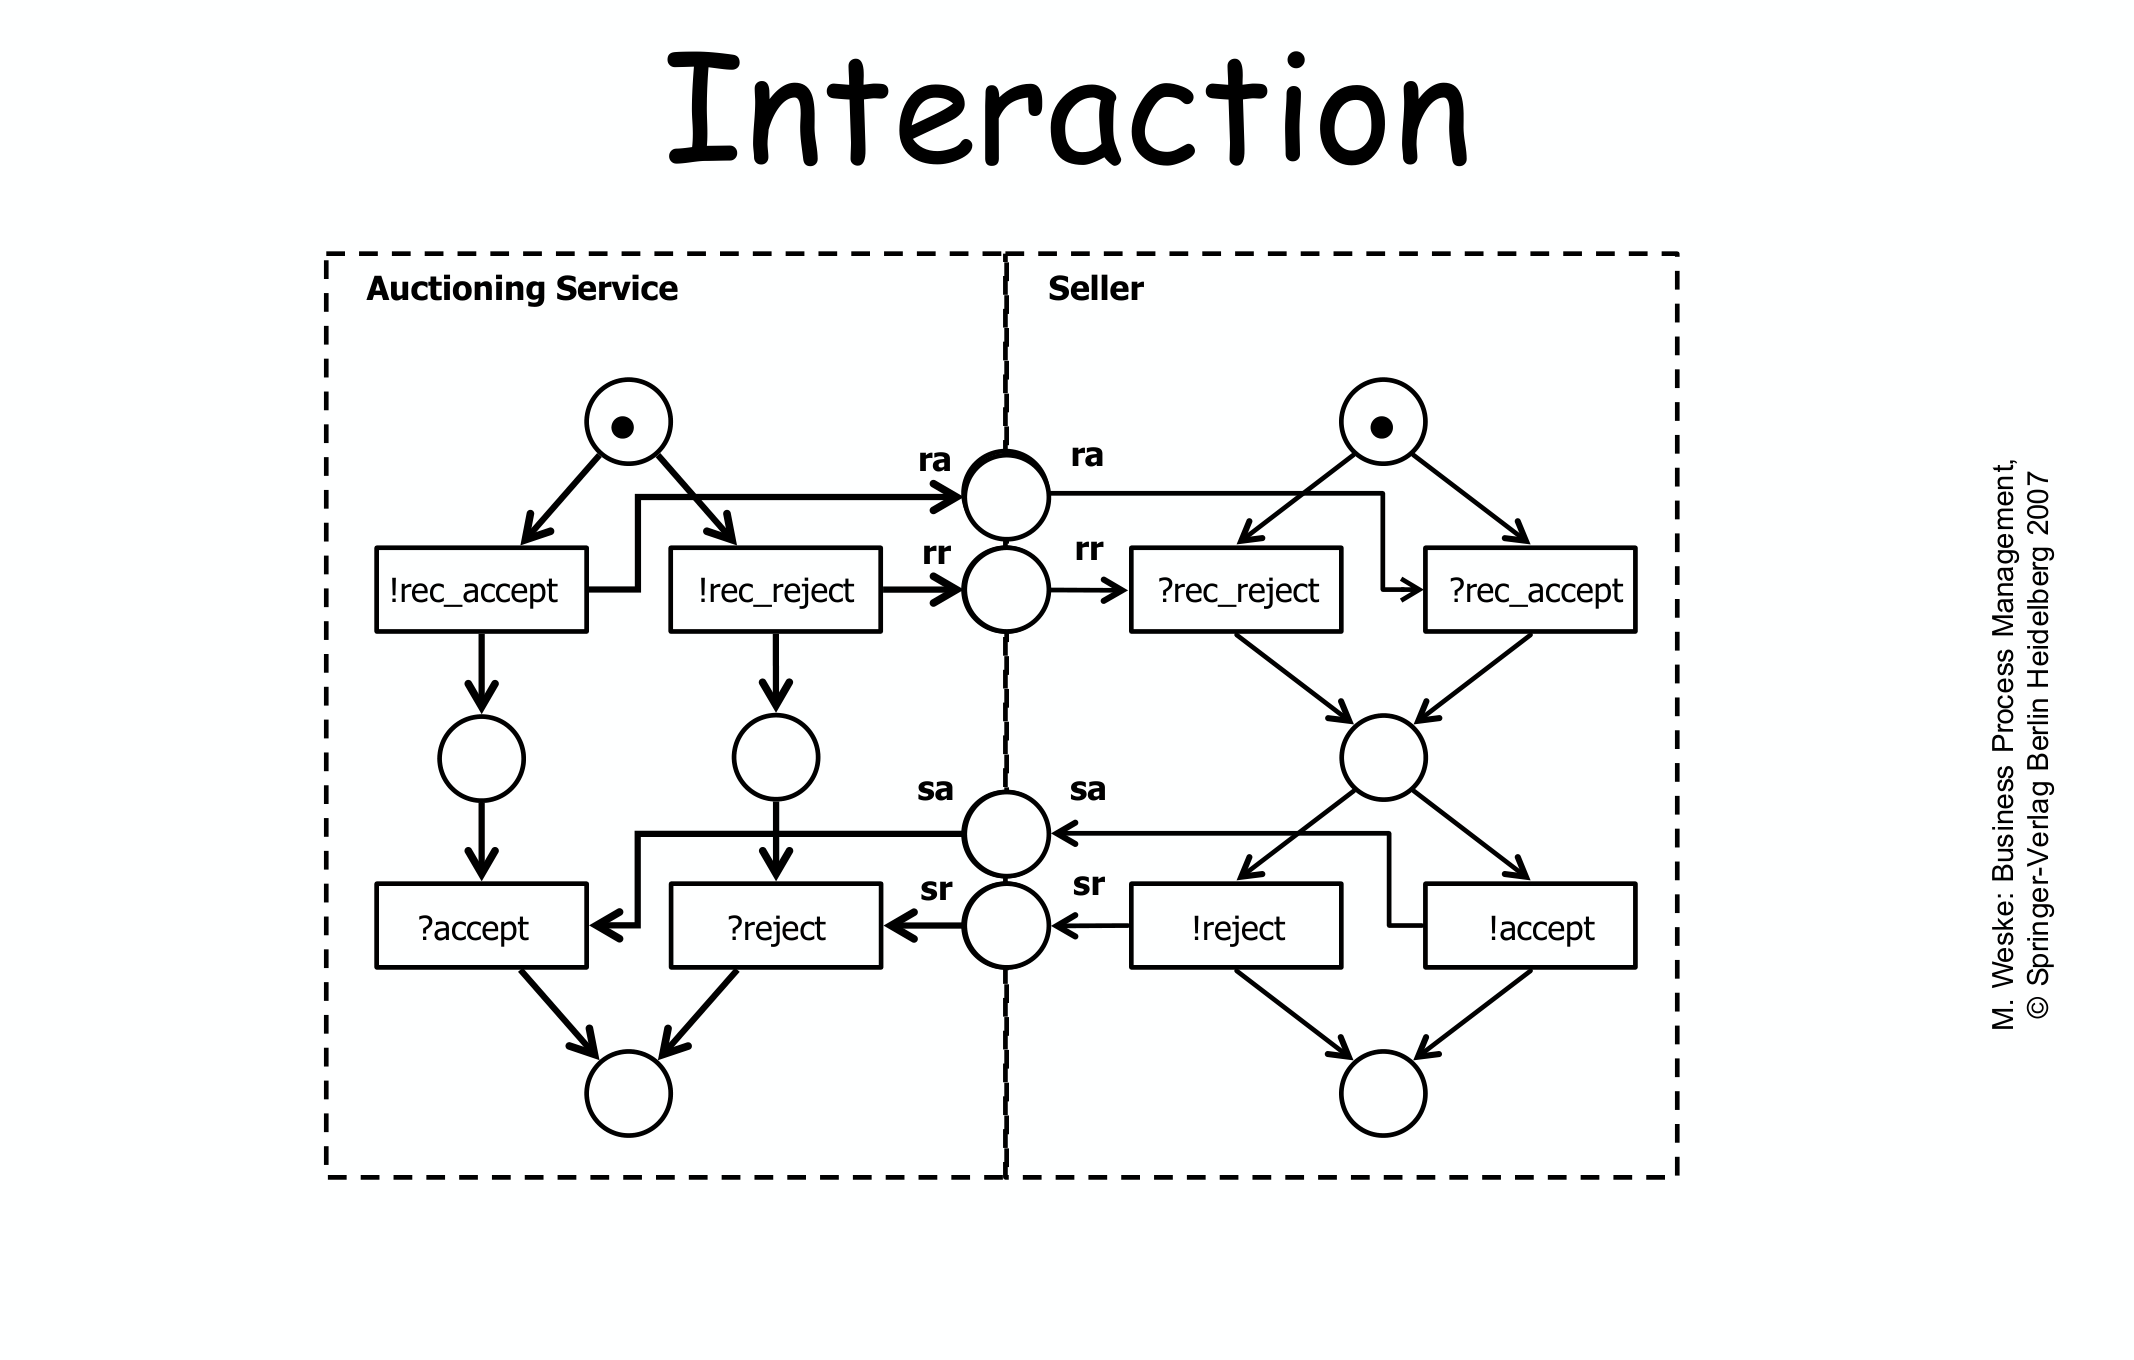
\includegraphics[width=0.74\linewidth,height=0.34\textheight,keepaspectratio]{images/18-workflow-systems_p11_interaction.png}
\caption{Dopo la fusione, i due moduli condividono i place centrali: è un'unica rete.}
\end{figure}

\begin{boxexample}{Passo 3 — chiudere e verificare la soundness}
Aggiungi un place iniziale $i$ e finale $o$ comuni:

\[
i \ \xrightarrow{\ t_i\ }\ (i_1,\dots,i_n) \qquad\qquad (o_1,\dots,o_n) \ \xrightarrow{\ t_o\ }\ o
\]

(come in \hyperref[ch:18]{18 — Workflow Systems}): il risultato è un workflow net ordinario, verificabile con la sezione 5.
\end{boxexample}

\begin{figure}[!htb]
\centering
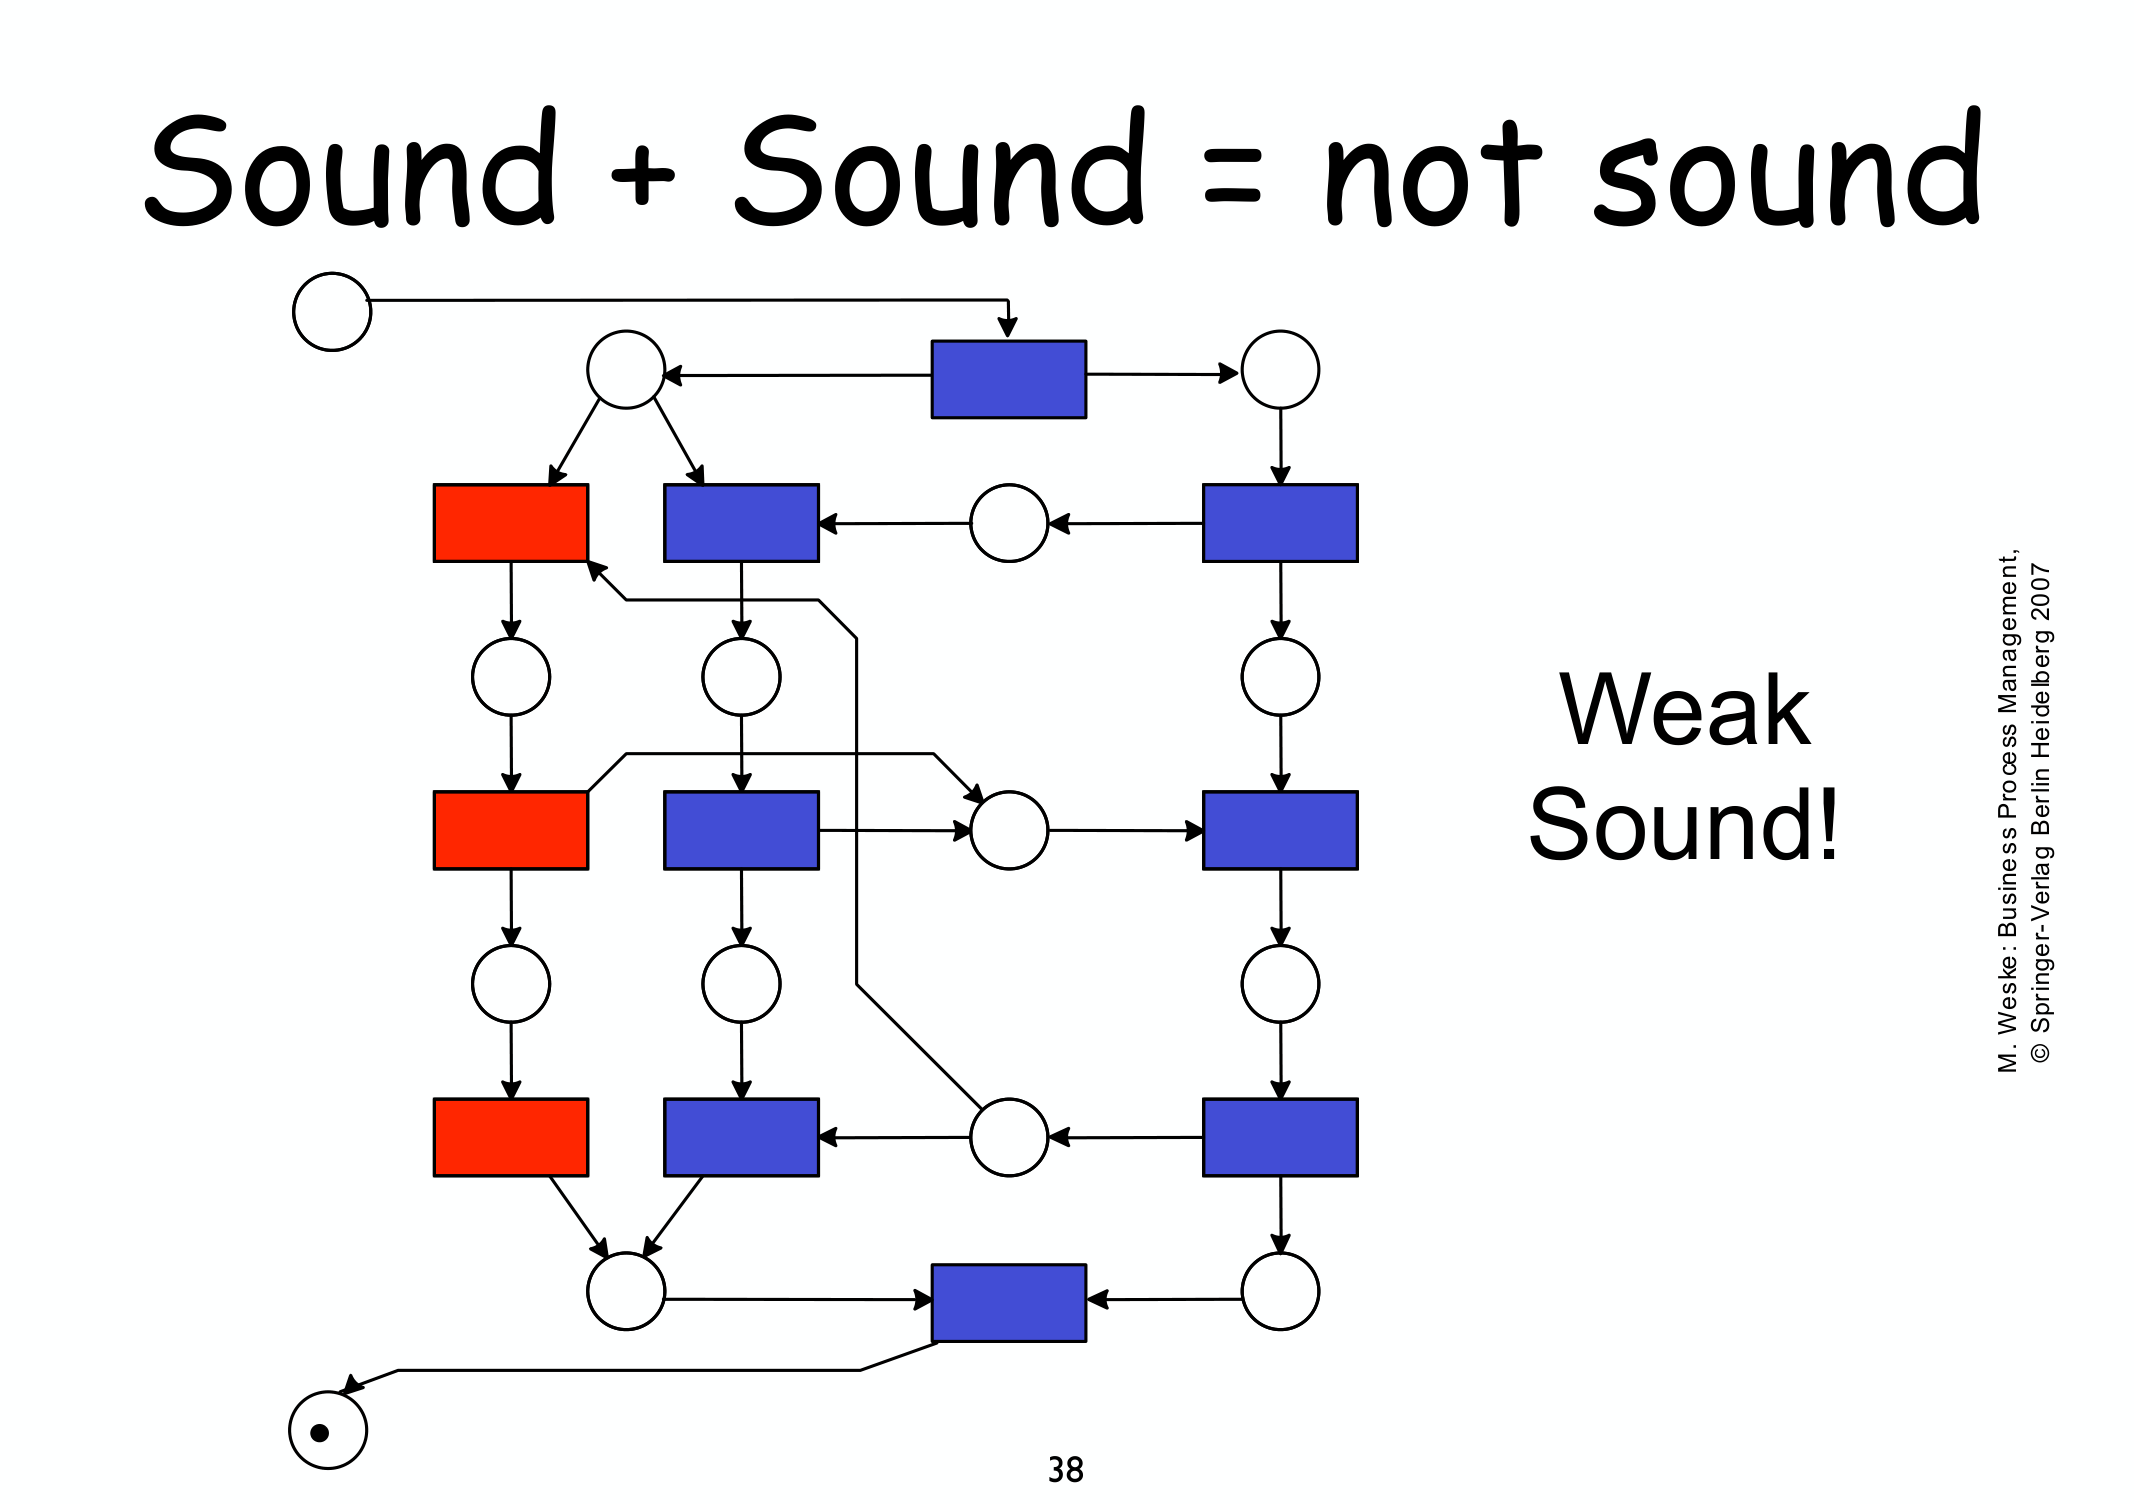
\includegraphics[width=0.74\linewidth,height=0.34\textheight,keepaspectratio]{images/18-workflow-systems_p38_soundplusound.png}
\caption{Il risultato sorprendente: Auctioning Service e Seller sono \textbf{entrambi sound} presi da soli, ma il sistema composto \textbf{non lo è}. È comunque \textbf{weak sound} (nessun deadlock, solo qualche task inutilizzato) — la lezione pratica: \textbf{verifica sempre il sistema composto}, mai solo i pezzi.}
\end{figure}

\section{\texorpdfstring{10. Conformance checking: token replay passo-passo}{10. Conformance checking: token replay passo-passo}}

\emph{Teoria: \hyperref[ch:19]{19 — Conformance}.}

Riproduciamo la trace $\sigma_3=\langle a,d,c,e,h\rangle$ su un modello dove l'ordine atteso sarebbe $a,c,d,e,h$ (cioè $c$ prima di $d$), contando \textbf{produced} ($p$), \textbf{consumed} ($c$), \textbf{missing} ($m$), \textbf{remaining} ($r$).

\begin{boxnote}{I quattro contatori}
\[
\text{fitness}(\sigma,N) = \frac12\left(1-\frac{m}{c}\right) + \frac12\left(1-\frac{r}{p}\right)
\]
\end{boxnote}

\begin{figure}[!htb]
\centering
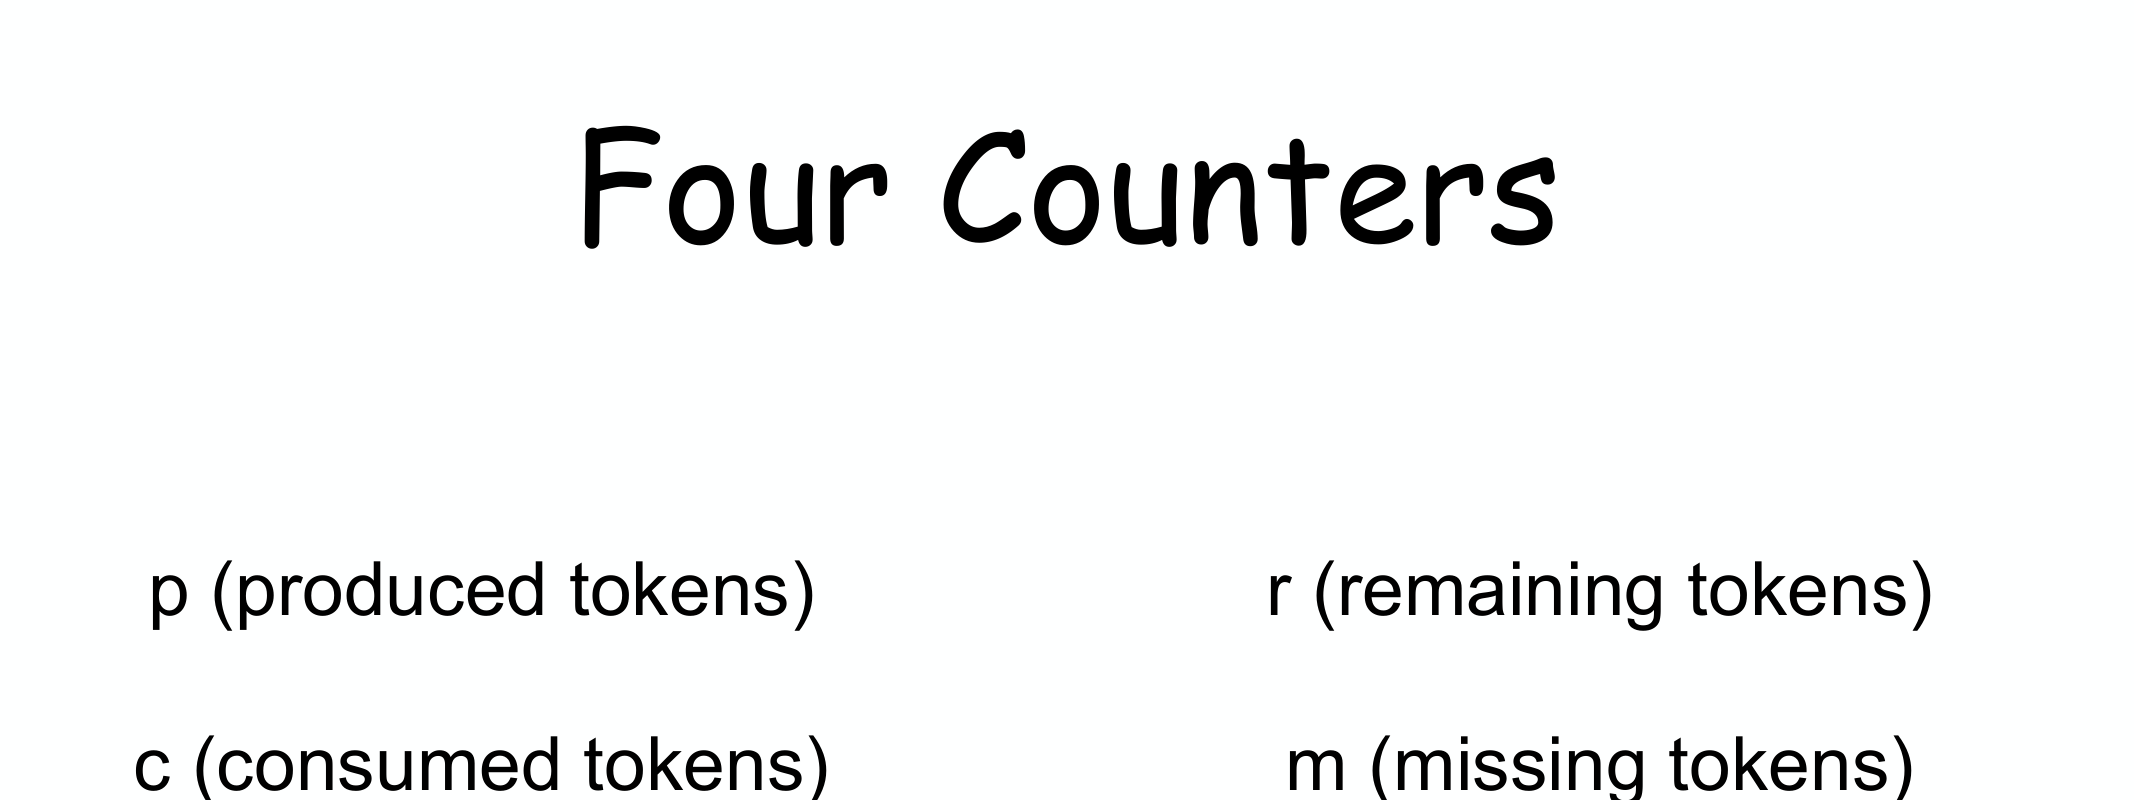
\includegraphics[width=0.74\linewidth,height=0.34\textheight,keepaspectratio]{images/19-conformance_p14_four-counters.png}
\caption{La rete di riferimento e la formula.}
\end{figure}

\begin{boxexample}{Riproduzione passo-passo di $\sigma_3=\langle a,d,c,e,h\rangle$}
\begin{enumerate}
\item \texttt{a}: consuma da \texttt{start}, produce due token (uno per il ramo b/c, uno per il ramo d) $\rightarrow$ nessun problema.
\item \texttt{d}: \textbf{dovrebbe} consumare da p2 (prodotto da \texttt{c}) — ma \texttt{c} non è ancora scattata! Il token \textbf{manca}: si forza comunque lo scatto e si incrementa $m$.
\item \texttt{c}: ora scatta regolarmente (il suo place di input aveva comunque il token dal passo 1).
\item \texttt{e}, \texttt{h}: proseguono regolarmente.
\end{enumerate}
\end{boxexample}

\begin{figure}[!htb]
\centering
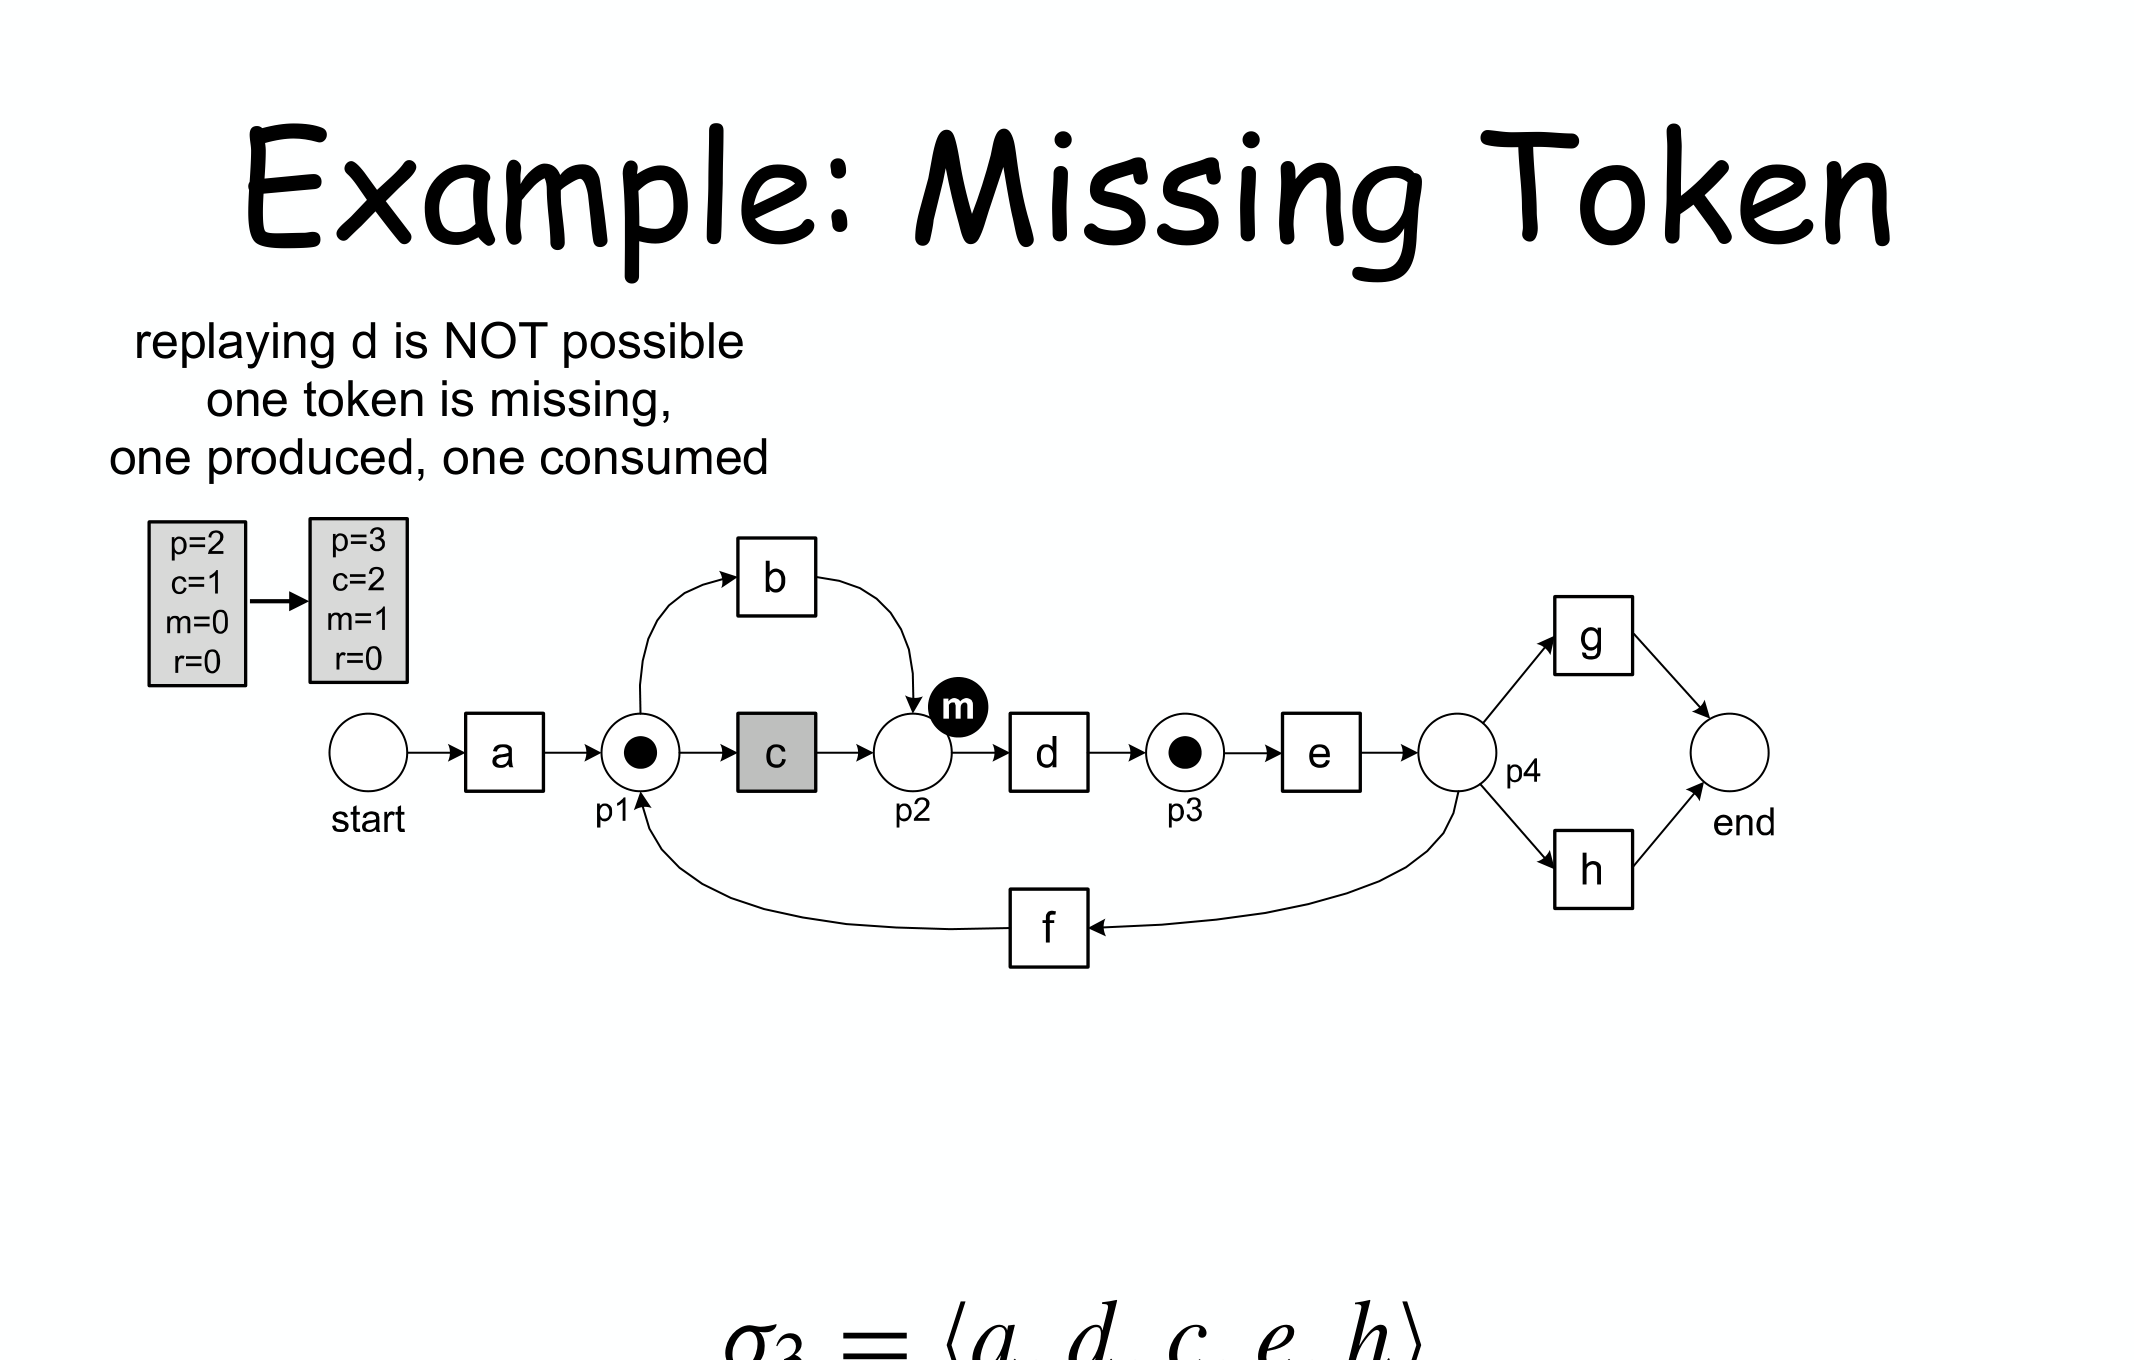
\includegraphics[width=0.74\linewidth,height=0.34\textheight,keepaspectratio]{images/19-conformance_p24_missing-token.png}
\caption{Il momento esatto del problema: uno solo dei quattro contatori si muove ($m$ passa da 0 a 1), il resto della riproduzione \textbf{continua} invece di fermarsi — a differenza della fitness ingenua, che avrebbe scartato l'intera trace al primo intoppo.}
\end{figure}

\[
\text{fitness}(\sigma_3,N) = \frac12\left(1-\frac16\right) + \frac12\left(1-\frac16\right) \approx 0.83
\]

Non perfetta, ma quantificata.

\begin{boxtip}{La procedura in breve}
Per ogni evento della trace, nell'ordine: (a) se il place di input ha il token, consumalo normalmente e produci in output ($p$ e $c$ crescono insieme); (b) se \textbf{manca}, forza comunque lo scatto e incrementa $m$; alla fine della trace, ogni token rimasto \textbf{nei place} (invece che consumato dall'ambiente) incrementa $r$.
\end{boxtip}

\section{\texorpdfstring{11. Flow analysis: calcolare il cycle time end-to-end}{11. Flow analysis: calcolare il cycle time end-to-end}}

\emph{Teoria: \hyperref[ch:20]{20 — Quantitative Analysis}.}

Le quattro regole: \textbf{sequenza} (somma), \textbf{XOR} (media pesata), \textbf{AND} (massimo), \textbf{rework} ($CT_P/(1-r)$). Componiamole su un unico processo:

\begin{center}
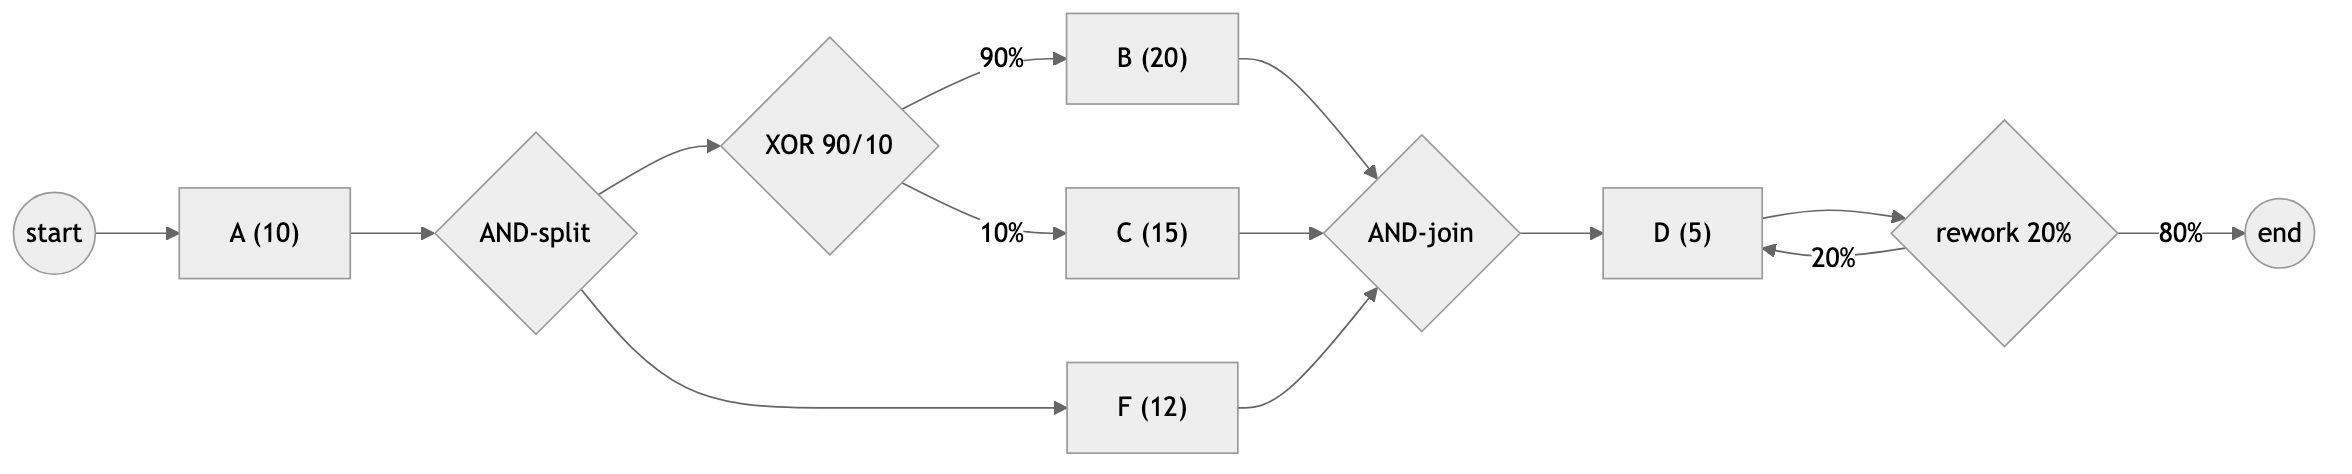
\includegraphics[width=0.74\linewidth,height=0.32\textheight,keepaspectratio]{images/mermaid/22_1.png}
\end{center}

\begin{boxexample}{Calcolo passo-passo (dal blocco più interno all'esterno)}
\textbf{1. XOR-block} (B/C, un ramo dell'AND-split):

\[
CT_{XOR} = 0.9\cdot20 + 0.1\cdot15 = 19.5
\]

\textbf{2. AND-block} (i due rami paralleli aperti dall'AND-split: lo XOR-block appena calcolato e il singolo task $F$) — vince il ramo più lento:

\[
CT_{AND} = \max\{CT_{XOR},\, CT_F\} = \max\{19.5,\ 12\} = 19.5
\]

\textbf{3. Rework loop su D} (0.2 di probabilità di ripetere):

\[
CT_D = \frac{5}{1-0.2}=6.25
\]

\textbf{4. Sequenza completa}:

\[
CT = CT_A + CT_{AND} + CT_D = 10+19.5+6.25 = 35.75
\]
\end{boxexample}

\begin{boxtip}{L'ordine di lavoro}
Risolvi sempre \textbf{dal blocco più interno verso l'esterno}: prima i rework loop e gli XOR/AND-block "foglia", poi sostituiscili con un singolo numero e tratta il resto come una sequenza. È lo stesso principio con cui si valuta un'espressione aritmetica annidata.
\end{boxtip}

\section{\texorpdfstring{12. S-coverability: costruire un S-cover per certificare la soundness}{12. S-coverability: costruire un S-cover per certificare la soundness}}

\emph{Teoria: \hyperref[ch:21]{21 — WFnets Diagnosis}.}

Vogliamo trovare, per una rete con 8 place ($s_1..s_8$) e 7 transition, un \textbf{S-invariant positivo} senza risolvere un sistema lineare — decomponendo in \textbf{S-component}.

\begin{boxexample}{Passo 1 — trovare un S-component}
Un S-component è un ciclo \textbf{S-net strongly connected} dove, se includi un place, devi includere \textbf{tutte} le sue transition.
\end{boxexample}

\begin{figure}[!htb]
\centering
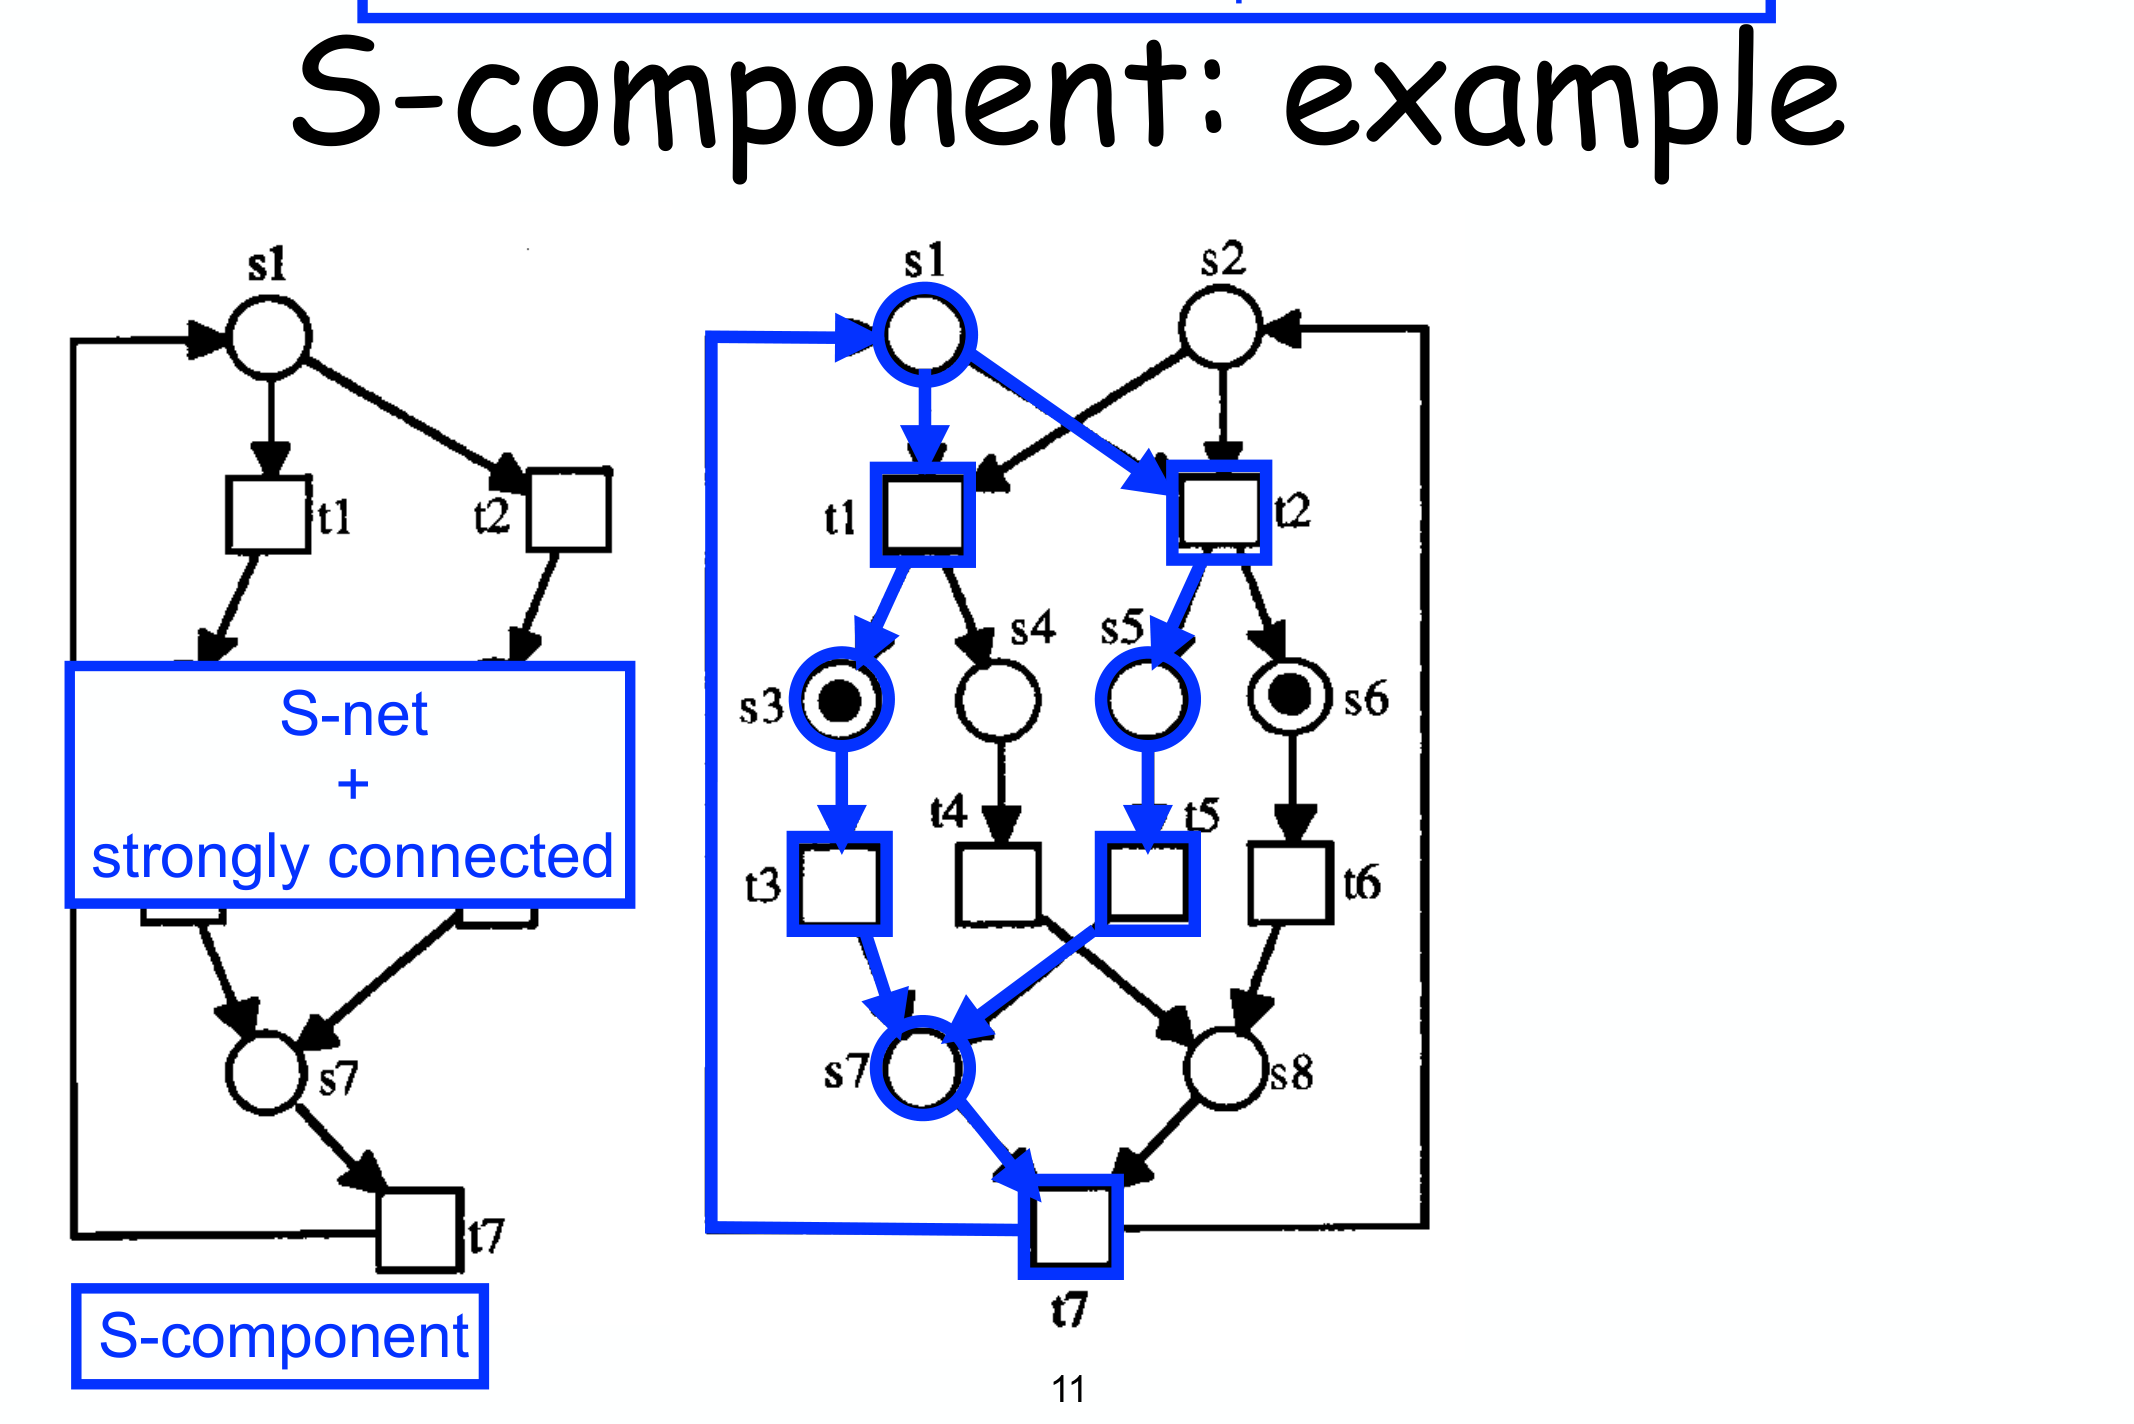
\includegraphics[width=0.74\linewidth,height=0.34\textheight,keepaspectratio]{images/21-wfnets-diagnosis_p11_s-component-example.png}
\caption{Il primo filone di controllo: $s_1 \to t_1 \to s_3 \to t_3 \to s_7 \to t_7 \to s_1$. Copre $s_1,s_3,s_7$ (e le transition associate) ma \textbf{non} $s_2,s_4,s_5,s_6,s_8$.}
\end{figure}

\begin{boxexample}{Passo 2 — trovare un secondo S-component che copra il resto}
Un secondo filone, simmetrico al primo, copre $s_2,s_4,s_5,s_6,s_8$.
\end{boxexample}

\begin{figure}[!htb]
\centering
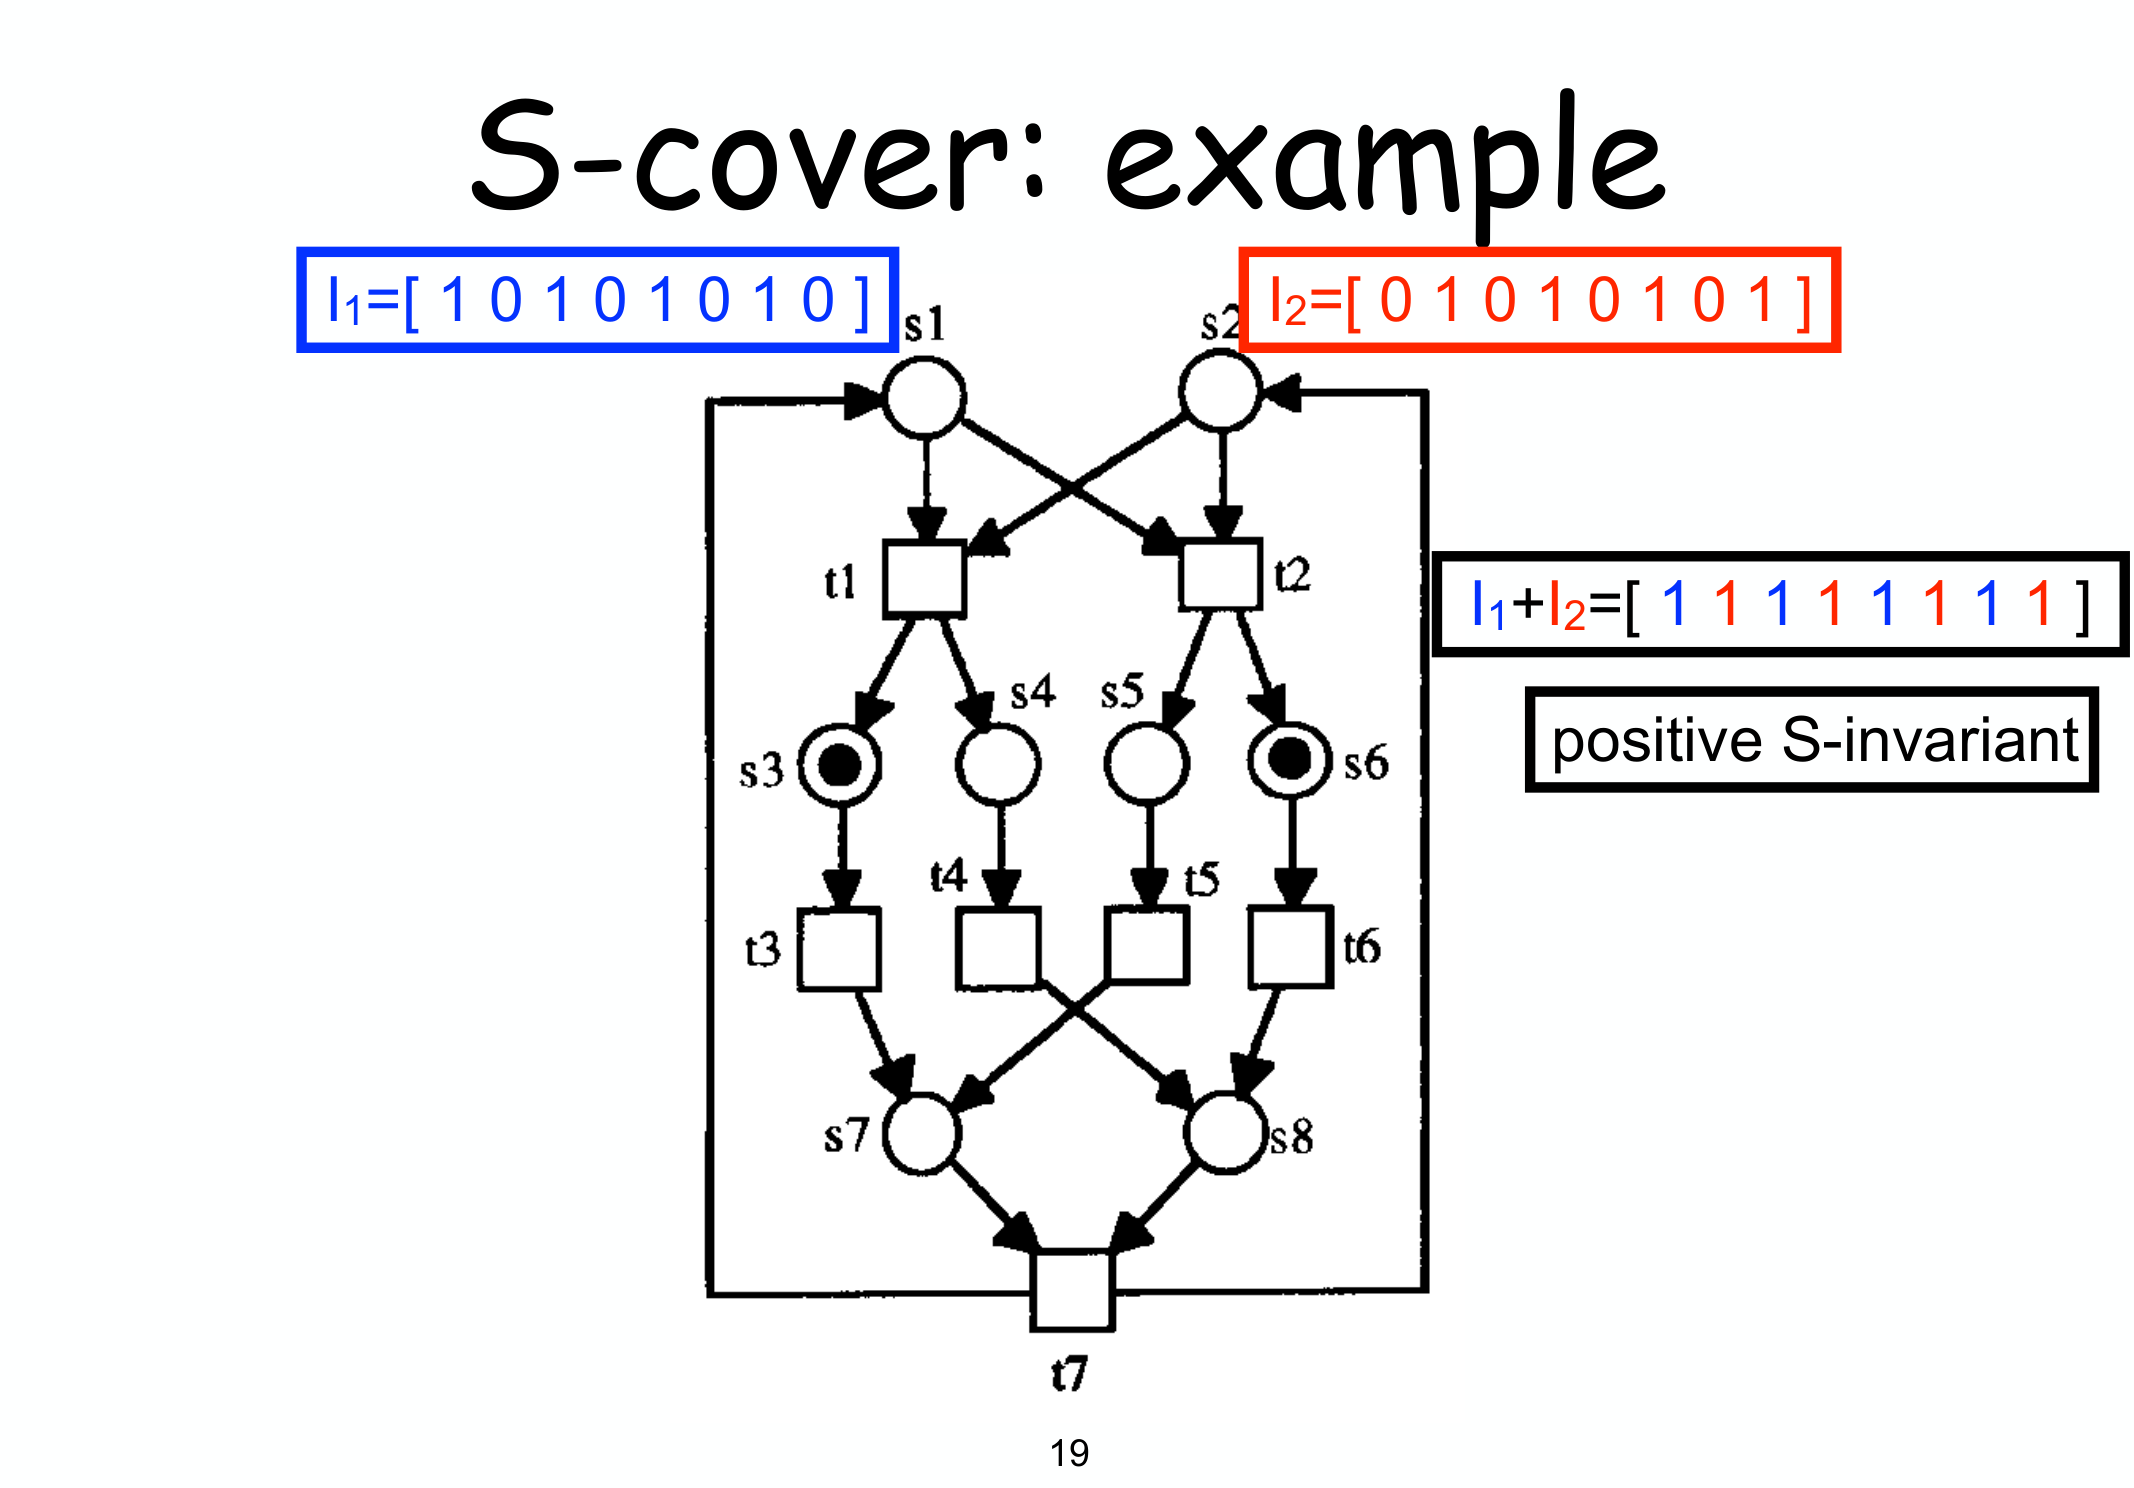
\includegraphics[width=0.74\linewidth,height=0.34\textheight,keepaspectratio]{images/21-wfnets-diagnosis_p19_s-cover-example.png}
\caption{Insieme, i due S-component formano un \textbf{S-cover} (ogni place coperto da almeno uno). Ciascuno induce un S-invariant uniforme, con peso 1 sui place coperti e 0 altrove (vettori sotto).}
\end{figure}

\begin{boxexample}{Passo 3 — sommare per ottenere un invariante positivo}
\[
\begin{array}{rcl}
I_1 &=& [1,0,1,0,1,0,1,0] \\
I_2 &=& [0,1,0,1,0,1,0,1] \\
\hline
I_1+I_2 &=& [1,1,1,1,1,1,1,1]
\end{array}
\]

\textbf{Tutti} i pesi sono positivi $\rightarrow$ \textbf{S-invariant positivo}, ottenuto senza risolvere alcun sistema lineare — solo disegnando due cicli e sommando due vettori 0/1.
\end{boxexample}

\begin{boxtip}{A cosa serve in pratica}
Se \textbf{riesci} a trovare un S-cover, hai certificato uno dei sei ingredienti del Rank Theorem con un disegno. Se \textbf{non ci riesci} (e la rete è free-choice), per il primo teorema di S-coverability concludi che la rete \textbf{non è live e bounded} — quindi il workflow net \textbf{non è sound} — senza nemmeno costruire il reachability graph.
\end{boxtip}